\documentclass[12pt,oneside]{report}

% ---------- Layout: single column, IEEE-influenced typography ----------
\usepackage[margin=1in]{geometry}
\usepackage{times}
\usepackage[T1]{fontenc}
\usepackage{graphicx}
\usepackage{titlesec}
\usepackage{fancyhdr}
\usepackage{setspace}
\usepackage{enumitem}
\usepackage{longtable}
\usepackage{booktabs}
\usepackage{array}
\usepackage{caption}
\usepackage{hyperref}
\usepackage{xcolor}
\usepackage{listings}
\usepackage{amsmath}
\usepackage{tocloft}

\hypersetup{
  colorlinks=true,
  linkcolor=black,
  citecolor=black,
  urlcolor=blue,
  pdftitle={Nexis: A Multi-Agent Autonomous Engineering Platform with Closed-Loop Fault Recovery},
  pdfauthor={Ratul Sikder}
}

\onehalfspacing
\setlength{\parindent}{0pt}
\setlength{\parskip}{8pt}

% Chapter/section heading style — plain, EduRide-style (not IEEE roman-numeral)
\titleformat{\chapter}[hang]{\LARGE\bfseries}{Chapter \thechapter}{1em}{}
\titlespacing*{\chapter}{0pt}{0pt}{24pt}
\titleformat{\section}{\Large\bfseries}{\thesection}{0.8em}{}
\titleformat{\subsection}{\large\bfseries}{\thesubsection}{0.8em}{}

\pagestyle{fancy}
\fancyhf{}
\fancyfoot[R]{Page \thepage\ of \pageref{LastPage}}
\renewcommand{\headrulewidth}{0pt}
\usepackage{lastpage}

\captionsetup{labelfont=bf,font=small}

\lstset{
  basicstyle=\ttfamily\footnotesize,
  breaklines=true,
  frame=single,
  columns=fullflexible,
  backgroundcolor=\color{gray!8},
  captionpos=b
}

\newcommand{\code}[1]{\texttt{#1}}

\begin{document}

% ======================= TITLE PAGE =======================
\begin{titlepage}
\begin{center}
\vspace*{0.3cm}
{\Large University of Dhaka}\\[4pt]
{\Large Institute of Information Technology (IIT)}\\[40pt]
{\large Project\\On}\\[10pt]
{\Large\bfseries ``Nexis: A Multi-Agent Autonomous Engineering Platform\\with Closed-Loop Fault Recovery''}\\[40pt]
{\large Submitted By}\\[10pt]
{\large Name: Ratul Sikder}\\
{\large Exam Roll: 2506102}\\[30pt]
{\normalsize A project submitted to the Institute of Information Technology (IIT), DU\\
for the partial fulfillment of the degree requirements.}\\[30pt]
{\large Supervised By}\\[10pt]
{\large \rule{6cm}{0.4pt}}\\[4pt]
{\normalsize Institute of Information Technology (IIT)}\\
{\normalsize University of Dhaka}\\[30pt]
{\normalsize Date: 11\textsuperscript{th} August, 2026}
\end{center}
\end{titlepage}

% ======================= ACKNOWLEDGEMENT =======================
\chapter*{Acknowledgement}
\addcontentsline{toc}{chapter}{Acknowledgement}
I would like to express my sincere gratitude to the faculty of the Institute of
Information Technology (IIT), University of Dhaka, for the academic environment
and guidance that made this project possible. Nexis grew out of a genuine,
recurring frustration familiar to every engineering team I have worked with or
studied: the gap between an AI tool that writes a function and a system that
actually closes the loop on a production failure. I am grateful for the freedom
to pursue that problem in depth, across nine cooperating agents, a real
multi-tenant control plane, and a working closed-loop deployment engine, rather
than a narrower proof of concept. I also thank my family for their patience
during the long build-and-verify cycles this project demanded.

% ======================= DECLARATION =======================
\chapter*{Declaration}
\addcontentsline{toc}{chapter}{Declaration}
This is to declare that this project is my original work. No part of this work
has been submitted elsewhere, partially or entirely, for the award of any other
degree or diploma. All project-related information will remain confidential and
shall not be disclosed without the formal consent of the project supervisor. The
plagiarism policy, as stated by the supervisor, has been maintained.

\vspace{40pt}
Student's Name: Ratul Sikder

\vspace{20pt}
Student's Signature: \rule{6cm}{0.4pt}

% ======================= SIGNATURE PAGE =======================
\chapter*{Signature Page}
\addcontentsline{toc}{chapter}{Signature Page}
\renewcommand{\arraystretch}{2.2}
\begin{tabular}{@{}p{4.4cm}p{0.4cm}p{9.7cm}@{}}
Project & : & Nexis: A Multi-Agent Autonomous Engineering Platform with Closed-Loop Fault Recovery \\
Student Name & : & Ratul Sikder \\
Exam Roll & : & 2506102 \\
Institute & : & Institute of Information Technology (IIT), University of Dhaka \\
Date of Submission & : & 11\textsuperscript{th} August, 2026 \\
Supervised By & : & \rule{6cm}{0.4pt} \\
\textbf{Supervisor's Approval} & : & \rule{6cm}{0.4pt} \\
\end{tabular}
\renewcommand{\arraystretch}{1}

% ======================= ABSTRACT =======================
\chapter*{Abstract}
\addcontentsline{toc}{chapter}{Abstract}
Modern software engineering teams spend an estimated 40--60\% of their time on
maintenance, debugging, and manual incident response rather than building new
capability. Existing AI-assisted developer tools -- code completion, automated
test generation, deployment dashboards -- address individual tasks in
isolation; none model the collaborative structure of a real engineering team,
and none close the loop between detecting a production failure and
autonomously repairing it. \textbf{Nexis} addresses both gaps at once. It
models a software engineering organisation as nine role-specialised
autonomous agents across two cooperating layers -- a five-agent Execution
Team (Architect, Backend, QA, DevOps, Data Engineer) and a four-agent
Self-Healing Loop (Sentinel, Pathfinder, Synthesiser, Validator) -- durably
orchestrated by Temporal and gated by a severity-routed human-in-the-loop
Approval Gate that supports Approve, Reject, and Modify (RLHF) decisions.
This report documents the complete, working system: a multi-tenant control
plane (Go, PostgreSQL with row-level security, Neo4j, Redis), a Docker
shadow-validation sandbox, a real GitHub-App-mediated GitOps deployment path,
a from-scratch Docker preview-deploy engine that clones, builds, and serves an
arbitrary connected repository and feeds its own build/runtime failures back
into the same self-healing pipeline, and a Next.js console spanning
authentication, RBAC, intelligent role recommendation, incident observability,
billing, and multi-provider integrations. Two live end-to-end recovery runs
against a local large language model are reported verbatim -- one correctly
timing out at the human approval gate, one succeeding fully from fault
detection through an approved, deployed patch in under two minutes -- alongside
a live, verified proof of the preview-deploy engine building and serving a
real public repository. The report is written as a candid engineering account:
what works is demonstrated with reproducible evidence, and what is
deliberately out of scope -- a fully credentialed production deployment to the
registered \texttt{nexis.sh} domain, and the human-subject NASA-TLX study --
is stated plainly rather than implied.

\vspace{10pt}
\textbf{Keywords:} Multi-agent systems, autonomous software engineering,
self-healing systems, closed-loop fault recovery, root-cause analysis,
LLM-guided program repair, DevOps automation, Temporal workflow orchestration,
human-in-the-loop AI, retrieval-augmented generation.


% ======================= TOC =======================
\tableofcontents
\listoffigures
\listoftables

% ======================= CHAPTERS =======================
\input{chapters/ch1_introduction}
\chapter{Literature Review}
\label{ch:literature}

\section{Overview}
\label{sec:lit-overview}

Nexis is a systems-integration project: its contribution lies in composing
established, well-engineered tools into a closed loop that none of them forms
on its own. Intellectual honesty therefore requires a clear account of what
each underlying tool already does, and where Nexis merely depends on it versus
where Nexis extends it. This section surveys the relevant landscape in that
spirit.

\textbf{LLM coding assistants.} GitHub Copilot~\cite{copilot} is the most
widely deployed AI pair-programming tool; it completes code and, in its agent
modes, drafts multi-file changes inside an editor session. It operates
entirely within the developer's authoring context: it never observes a
production incident, never validates its own output against a failing system,
and never deploys anything. Nexis's Backend agent occupies the same
``generate a minimal code change'' niche, but is invoked by a fault-detection
pipeline rather than a keystroke, and its output is machine-validated before
any human sees it.

\textbf{Durable workflow orchestration.} Temporal~\cite{temporal} provides
durable, replayable workflow execution with automatic retry and state
persistence. Nexis uses Temporal as-is, as a dependency: the entire nine-agent
RecoveryPipeline is a Temporal workflow, which is why every agent step
survives process restarts and is recorded as a durable ActivityEvent. The
workflow's engineering semantics -- role routing, contract-violation
detection, severity classification -- are Nexis's own logic layered on top.

\textbf{Graph databases for dependency analysis.} Neo4j~\cite{neo4j} is a
native graph database. Nexis stores its code-dependency graph in Neo4j and
the Pathfinder agent walks it from a fault symptom to candidate root-cause
nodes, forwarding hop distance and node degree as evidence. Neo4j is a
storage and traversal dependency; the evidence-ranking performed on the
traversal results is Nexis code.

\textbf{Causal inference tooling.} DoWhy~\cite{dowhy} is Microsoft
Research's library for explicit causal modelling with refutation tests. It is
the methodological reference point for Nexis's causal-inference sidecar, but
it must be stated plainly that Nexis does \emph{not} fit a DoWhy structural
causal model: no interventional production data exists to fit one against.
The sidecar instead implements a documented proxy -- ranking candidates by
evidence-chain specificity, graph-structural proximity, textual overlap, and
a scenario prior, with a transparent per-component confidence breakdown.

\textbf{Observability standards.} OpenTelemetry~\cite{otel} standardises
traces, metrics, and logs. Nexis adopts it as its instrumentation layer
(exported to Prometheus, Loki, and Tempo behind Grafana). It is a
dependency; Nexis adds nothing to the standard itself.

\textbf{GitOps deployment.} Argo CD~\cite{argocd} reconciles a cluster
against a Git repository and exposes Sync and Rollback operations. Nexis's
DevOps agent emits Argo CD manifests, and the post-deploy rollback probe
calls Argo CD's real Rollback client when a policy-gated SLO breach is
detected -- integration, not extension.

\textbf{Container runtimes.} Docker~\cite{docker} is the target API for both
the Validator's sandbox (network-isolated, read-only, capability-dropped
shadow execution of every candidate patch) and the preview-deploy engine.
Podman~\cite{podman} was substituted in the evaluation environment as a
Docker-API-compatible runtime and behaved identically; this substitution is
reported honestly rather than hidden.

\textbf{Property-based testing.} Hypothesis~\cite{hypothesis} generates test
inputs from declared properties. Nexis's QA agent auto-generates
pytest/Hypothesis suites from the incident and the Backend diff -- a novel
\emph{use} of the library, with Hypothesis itself unmodified. A background QA
loop replays stored suites and raises a fresh incident on a pass-to-fail
regression.

\textbf{Data lineage.} OpenLineage~\cite{openlineage} defines an open
specification for run-level lineage events. Nexis's Data Engineer agent emits
OpenLineage-compatible RunEvents for every migration it proposes or applies;
Nexis conforms to the specification rather than extending it.

\textbf{The incident-response ecosystem.} Sentry~\cite{sentry},
Datadog~\cite{datadog}, and PagerDuty~\cite{pagerduty} respectively capture
application errors, aggregate observability data, and route alerts to on-call
humans. All three are integrated into Nexis as webhook-driven incident
\emph{sources} feeding the same Sentinel pipeline. The Slack
API~\cite{slackapi} is used in the opposite direction: the Approval Gate
pushes a decision into Slack, where an engineer can approve or reject a
validated patch with one click. Supporting platform dependencies -- WorkOS
for SSO~\cite{workos}, Stripe for billing~\cite{stripe}, PostgreSQL
row-level security for tenant isolation~\cite{pgrls}, pgvector for
knowledge-base retrieval~\cite{pgvector}, and Ollama~\cite{ollama} as the
local LLM provider used for this report's live evidence -- are used as
documented, without modification. Table~\ref{tab:lit-tools} summarises the
dependency-versus-contribution boundary.

\begin{table}[htbp]
\caption{Position of surveyed tools relative to Nexis.}
\label{tab:lit-tools}
\centering
\small
\begin{tabular}{@{}lll@{}}
\toprule
\textbf{Tool} & \textbf{What it provides} & \textbf{Relation to Nexis} \\
\midrule
Copilot~\cite{copilot} & Editor-time code generation & Comparable to one agent (Backend) only \\
Temporal~\cite{temporal} & Durable workflow execution & Dependency; hosts the RecoveryPipeline \\
Neo4j~\cite{neo4j} & Graph storage and traversal & Dependency; Pathfinder walks it \\
DoWhy~\cite{dowhy} & Structural causal models & Reference point; proxy method used instead \\
OpenTelemetry~\cite{otel} & Telemetry standard & Dependency; instrumentation layer \\
Argo CD~\cite{argocd} & GitOps sync/rollback & Integrated by DevOps agent and rollback probe \\
Docker~\cite{docker}/Podman~\cite{podman} & Container runtime & Dependency; sandbox and deploy engine \\
Hypothesis~\cite{hypothesis} & Property-based testing & Novel use: QA agent generates suites \\
OpenLineage~\cite{openlineage} & Lineage specification & Conformance by Data Engineer agent \\
Sentry/Datadog/PagerDuty~\cite{sentry,datadog,pagerduty} & Error/alert capture & Webhook incident sources \\
Slack API~\cite{slackapi} & Team messaging & One-click approval channel \\
\bottomrule
\end{tabular}
\end{table}

\section{Research Gap}
\label{sec:lit-gap}

Each tool above is strong within its boundary, and several are routinely
combined in industry -- Sentry alerting into PagerDuty, an on-call engineer
opening an editor with Copilot, Argo CD deploying the eventual merge. What no
single tool, and no combination in common use, provides is a system that
(a)~models a software engineering \emph{team} with explicit role
specialisation, and (b)~closes the loop from automatic fault detection to a
deployed, verified fix, with human judgement concentrated at one
severity-routed decision point.

The gap is visible at every seam of the conventional tool chain. Copilot
generates code but never sees a production incident; it has no notion of a
fault, a blast radius, or a deployment~\cite{copilot}. Observability
platforms such as Datadog and Sentry detect and display faults with great
fidelity but never generate a candidate fix, let alone validate
one~\cite{datadog,sentry}. PagerDuty routes a human to the problem; the
repair itself remains entirely manual~\cite{pagerduty}. Argo CD deploys
whatever a repository contains but authors nothing~\cite{argocd}. Temporal
can durably orchestrate any of these steps but carries no engineering
semantics of its own~\cite{temporal}. In every case the loop is broken at
the same place: between ``a fault is known'' and ``a validated fix exists,''
a human performs unaided diagnosis, authoring, testing, review, and release.

Nexis closes precisely that span, end to end. Sentinel detects a fault using
a statistical-process-control rule (an EWMA baseline with a
mean-plus-three-sigma breach condition), not a fixed threshold. Pathfinder
walks the real Neo4j dependency graph to candidate root causes, which the
causal-inference sidecar ranks with a transparent confidence breakdown. The
Synthesiser classifies the scenario and selects which Execution Team agents
are actually needed -- and the workflow enforces that routing, visibly
skipping unselected agents. The Architect produces a structured plan whose
\code{affected\_files} contract is mechanically checked against the Backend
agent's actual diff; a violation forces HIGH severity so the change can never
auto-deploy unreviewed. QA generates property-based tests from the incident
and the diff~\cite{hypothesis}; the Validator executes patch and tests in a
locked-down container sandbox, so no unvalidated patch ever reaches a human.
Only then does the single human decision point engage -- and only when
severity warrants it: HIGH-severity changes require explicit review,
MEDIUM-severity changes auto-approve after a 120-second window unless
overridden, and trivial LOW-severity changes pass immediately. The decision
itself is richer than a binary gate: the engineer may Approve, Reject, or
Modify the diff before it ships, with every terminal decision persisted for
future preference learning. On approval, a real GitHub pull request is opened
and a post-deploy rollback probe watches for regression~\cite{argocd}.

Two further properties distinguish this from a scripted pipeline of existing
tools. First, role specialisation is structural, not cosmetic: five Execution
Team agents (Architect, Backend, QA, DevOps, Data Engineer) and four
Self-Healing Loop agents (Sentinel, Pathfinder, Synthesiser, Validator) have
distinct inputs, outputs, and contracts, and the Architect's plan constrains
the others. Second, the loop is closed over the platform's own
infrastructure: when Nexis's preview-deploy engine fails to build or
health-check a repository, that failure is inserted as a first-class incident
into the very same pipeline, and ``write a working Dockerfile'' becomes an
ordinary repair task. To the author's knowledge, no tool in common use today
combines these properties in a single system.

\section{Conclusion}
\label{sec:lit-conclusion}

The surveyed landscape supplies every ingredient Nexis needs -- durable
orchestration~\cite{temporal}, graph traversal~\cite{neo4j}, sandboxed
execution~\cite{docker,podman}, property-based testing~\cite{hypothesis},
GitOps delivery~\cite{argocd}, and a mature incident-capture
ecosystem~\cite{sentry,datadog,pagerduty} -- but leaves the loop between
detection and repair open, to be closed by a human. Nexis's contribution is
not any single new algorithm; it is the demonstrated composition of these
tools into a role-specialised multi-agent team that detects, diagnoses,
repairs, validates, and deploys autonomously, engaging human judgement once,
at a severity-routed gate. The remaining chapters describe how that
composition was specified, designed, implemented, and tested.

\chapter{System Analysis and Requirements}

\section{Requirement Analysis}

Nexis is a role-based, multi-tenant platform. Every piece of data in the
system belongs to exactly one organisation (tenant), and every request is
evaluated against both the caller's organisation and the caller's role within
it. The requirement analysis therefore begins by identifying the actors who
interact with the system boundary.

Three \emph{human} actor types were identified:

\begin{itemize}[nosep]
  \item \textbf{Owner/Admin} --- the organisation's administrator, responsible
        for membership, roles, billing, policy, integrations, and the final
        human decision on high-stakes automated repairs.
  \item \textbf{Engineer/Member} --- the working engineer who investigates
        incidents, exercises the evaluation tooling, and interacts with the
        recovery pipeline day to day.
  \item \textbf{Viewer} --- a read-only observer (for example a stakeholder or
        an auditor) who may inspect the system's state but may not change it.
\end{itemize}

The role model is \emph{additive}: an Admin holds every permission an Engineer
holds, and an Engineer holds every permission a Viewer holds. Consequently,
the functional requirements in Section~3.2 list only the permissions each role
\emph{adds} to the tier below it, without repetition. (Internally the database
role enumeration is owner/admin/member; the console additionally presents the
read-only Viewer experience through RBAC gating on the frontend and API.)

Unusually for a requirement analysis, a fourth actor category must be modelled
that is not human at all: the \textbf{nine-agent self-healing fleet}. Most
requirement-analysis chapters enumerate only human actors, because in a
conventional system every state change ultimately traces back to a person
clicking something. That assumption does not hold for Nexis. The agent fleet
acts autonomously inside the system boundary: it detects faults without being
asked, reads and writes the same PostgreSQL, Neo4j, and object-storage data
stores the human-facing console uses, and triggers real external side effects
--- opening GitHub pull requests, applying rollbacks through Argo
CD~\cite{argocd}, and redeploying preview containers. An actor model that
omitted the fleet would misrepresent the system: roughly half of all writes to
the incident, patch, and audit tables originate from agents rather than
people. Treating the fleet as a first-class actor also makes the safety
analysis explicit --- every autonomous capability listed in Section~3.2.4 is
bounded by a corresponding control (sandboxing, severity classification, or
the human approval gate) listed in Section~3.3.

The Level~0 and Level~1 use case diagrams for these four actors are presented
together with the rest of the system's UML design in
Section~\ref{sec:usecase-diagrams} (Figures~\ref{fig:usecase-l0} and
\ref{fig:usecase-l1}), alongside the data flow diagrams that show how the same
actors move data through the platform.

\section{Functional Requirements}

The functional requirements are grouped by actor. Because the role model is
additive, each human tier is listed as a delta over the tier below it.

\subsection{Owner/Admin can:}

\begin{itemize}[nosep]
  \item Do everything an Engineer/Member and a Viewer can do (role
        additivity).
  \item Manage organisation membership: generate invite codes, send email
        invites, and remove members.
  \item Assign and change member roles, and act on the intelligent
        role-recommendation banner on the Members settings page --- accepting
        a recommendation (which applies the role change under an
        optimistic-concurrency guard) or dismissing it (which starts a 30-day
        per-rule cool-down).
  \item Edit organisation settings (name, profile, and workspace-level
        configuration).
  \item Manage billing through Stripe~\cite{stripe}: view usage, manage
        payment methods, and review invoices produced by the usage-ticker and
        invoice-roller cron jobs; set the organisation's daily token budget on
        the cost tracker.
  \item View and export the append-only, hash-chained audit log (CSV export)
        and invoke its cryptographic verification endpoint to prove the chain
        has not been tampered with.
  \item Decide pending approvals from the recovery pipeline: \textbf{Approve}
        a validated patch, \textbf{Reject} it, or \textbf{Modify} it --- edit
        the unified diff in place before it ships, with the edited diff
        persisted as an RLHF feedback example.
  \item Configure each project's recovery policy, including
        rollback-on-SLO-breach behaviour.
  \item Operate the Docker preview-deploy engine from a project's
        \emph{Ops} tab: trigger Deploy and Stop, watch live status, open the
        returned preview URL, inspect build and container logs, and review
        deployment history.
  \item Install and manage integrations: the GitHub App (installation, repo
        listing, webhook-driven incident creation on merged pull requests),
        Sentry~\cite{sentry}, Datadog~\cite{datadog}, and
        PagerDuty~\cite{pagerduty} webhook sources, Slack~\cite{slackapi}
        (OAuth install plus interactive one-click approve/reject directly
        from a Slack message), and Argo CD~\cite{argocd}.
  \item Export evaluation-harness results as CSV (an admin-only action).
  \item Receive the daily admin digest e-mail summarising the last 24 hours
        of incidents, repairs, approvals, and MTTR for the organisation.
  \item Monitor platform operations pages: System Health (parallel dependency
        probes of PostgreSQL, Redis, Neo4j, MinIO, and Temporal), webhook
        activity, and integration connection health.
\end{itemize}

\subsection{Engineer/Member can:}

\begin{itemize}[nosep]
  \item Do everything a Viewer can do (role additivity).
  \item Sign up and sign in with e-mail and password (JWT session in an
        HttpOnly cookie), sign in passwordlessly via magic link, or sign in
        through WorkOS SSO~\cite{workos}; recover access through the
        password-reset flow (hashed, time-limited reset tokens).
  \item Enrol multi-factor authentication (TOTP with QR provisioning).
  \item Manage their own active sessions: list signed-in devices with IP
        address, user agent, and last-seen time (the caller's own session
        carries a ``This device'' badge), and revoke any session remotely.
  \item Create, list, and revoke scoped API keys (\code{nx\_live\_\ldots}
        bearer tokens) for programmatic access.
  \item Create projects through the new-project wizard and connect them to
        GitHub repositories.
  \item Browse the incidents list and open an incident's detail page, where
        the nine-agent pipeline timeline streams live over Server-Sent
        Events, including per-agent status, token counts, and cost.
  \item Inspect each agent's structured payloads (for example the Backend
        agent's raw generated diff) from the timeline.
  \item Trigger fault-injection runs from the Live-Demo console page, which
        presents 27 curated scenario cards drawn from a broader
        fixture-scenario taxonomy (one scenario is fully wired end-to-end
        today; the remainder are labelled ``Coming soon'').
  \item Run the evaluation harness: side-by-side OpenAI-versus-Ollama
        provider comparisons over fixture incidents, with persisted
        transcripts and cost figures.
  \item Query the knowledge base (pgvector-backed retrieval~\cite{pgvector})
        and view its retrieval status.
  \item Complete the post-incident NASA-TLX workload survey~\cite{nasatlx},
        the platform's instrument for measuring operator cognitive load.
  \item Use the operational consoles: the agents fleet page and per-agent
        detail views, the workflows list, the activity stream, the validator
        sandbox page, and the recovery-pipeline view.
\end{itemize}

\subsection{Viewer can:}

\begin{itemize}[nosep]
  \item Sign in and view the dashboard: KPI tiles (MTTR, recovery success
        rate, open incidents, mean tokens per run), the incidents-over-time
        chart, the system status panel, the projects health grid, and the
        recent activity feed.
  \item Read the incidents list and incident detail timelines, including the
        live SSE stream, without any decision or mutation controls.
  \item Read project pages (overview, activity, and status) and the
        performance page.
  \item View the agents, workflows, and activity-stream pages in read-only
        form.
  \item Take no mutating action of any kind: no approvals, no deployments, no
        settings changes, no key or session management beyond their own
        account.
\end{itemize}

\subsection{The 9-Agent Fleet autonomously:}

\begin{itemize}[nosep]
  \item \textbf{Detects} faults (Sentinel): an always-on detector applies two
        rules --- a per-row fatal-level trigger, and a statistical-process-%
        control spike rule that maintains a per-organisation EWMA mean and
        variance baseline and fires on a breach of mean~$+3\sigma$, with a
        Poisson floor for low-count noise and an absolute-floor warm-up
        fallback.
  \item \textbf{Diagnoses} root causes (Pathfinder): walks the Neo4j code
        dependency graph~\cite{neo4j} outward from the fault symptom and
        forwards candidate root-cause nodes, annotated with hop distance and
        degree, to the causal-inference sidecar, which ranks candidates by
        evidence-chain specificity, structural proximity, textual overlap,
        and a scenario prior, returning a per-component confidence
        breakdown~\cite{dowhy}.
  \item \textbf{Classifies and routes} (Synthesiser): assigns the incident a
        scenario (regex fast path with LLM fallback) and computes an ordered
        \code{selected\_agents} list; the workflow enforces this routing,
        skipping non-selected execution agents with a visible ``skipped''
        timeline state.
  \item \textbf{Plans} the repair (Architect): decomposes the incident into
        \code{plan\_steps}, \code{affected\_files}, and a
        \code{risk\_level}, and serves as a contract other agents may not
        silently violate --- if the generated diff touches a file outside
        \code{affected\_files}, the workflow flags a contract violation and
        forces HIGH severity so the patch can never auto-deploy unreviewed.
  \item \textbf{Codes} the fix (Backend): generates an LLM-guided minimal
        unified diff --- the smallest valid change rather than a full-file
        rewrite.
  \item \textbf{Tests} the fix (QA): auto-generates property-based test
        suites (pytest/Hypothesis~\cite{hypothesis}) from the incident and
        the diff; a background continuous-QA loop replays previously
        generated suites against the sandbox and raises a fresh incident on
        any pass-to-fail regression, closing a second, independent loop.
  \item \textbf{Packages} the deployment (DevOps): emits CI/CD and Argo CD
        manifests~\cite{argocd} and drives post-deployment health
        monitoring.
  \item \textbf{Handles data changes} (Data Engineer): proposes paired
        forward and reverse SQL migrations, runs a proactive schema-drift
        detector that introspects \code{information\_schema} against a
        captured baseline and raises a real incident on drift, and emits
        OpenLineage-compatible run events~\cite{openlineage} for every
        migration proposal and application.
  \item \textbf{Validates} every candidate patch (Validator): executes it in
        a locked-down Docker sandbox~\cite{docker} (no network, read-only
        filesystem, all capabilities dropped, PID-limited,
        no-new-privileges), runs the QA-generated property tests, and reports
        pass/fail and coverage; no unvalidated patch ever reaches the
        approval gate.
  \item \textbf{Classifies severity} at the approval gate: HIGH for
        schema-drift scenarios, sensitive-path matches (SQL, migrations,
        auth, security, crypto), unknown scenarios, or contract violations;
        MEDIUM otherwise, with a 120-second auto-approve countdown unless a
        human intervenes; LOW (tiny UI-only diffs) auto-approves immediately.
  \item \textbf{Deploys} approved patches (GitOps): opens a real GitHub pull
        request through a GitHub App installation
        (blob$\rightarrow$tree$\rightarrow$commit$\rightarrow$ref$\rightarrow$PR);
        when the triggering incident originated from the preview-deploy
        engine, a successful merge additionally triggers an automatic
        redeploy.
  \item \textbf{Rolls back} on regression: a post-deploy probe watches for a
        fresh fatal incident on the same organisation and service within a
        bounded window and, when the project policy permits, invokes Argo
        CD's rollback client to restore the prior known-good revision.
  \item \textbf{Records} every step as a Temporal-durable activity
        event~\cite{temporal} and streams it live to the incident detail
        page over Server-Sent Events.
  \item \textbf{Feeds the deploy engine's failures back into itself}: when a
        preview deployment fails to build or pass its health check, the
        deploy engine files a real incident (\code{source:
        "deploy\_engine"}) into the same Sentinel-to-pipeline path as every
        other incident source, making a broken build a self-healing target
        like any production fault.
\end{itemize}

\section{Non-Functional Requirements}

\begin{table}[htbp]
\caption{Summary of non-functional requirements and their realisation.}
\label{tab:nfr}
\centering
\begin{tabular}{p{3.4cm}p{9.6cm}}
\toprule
\textbf{Requirement} & \textbf{Realisation in Nexis} \\
\midrule
Multi-tenancy & PostgreSQL Row-Level Security on essentially every table~\cite{pgrls} \\
Durability & Temporal-orchestrated workflows survive crashes and restarts~\cite{temporal} \\
Security & Sandboxed patch execution, encrypted patch storage, hashed tokens, hash-chained audit log \\
Scalability & Stateless Go services, queue-decoupled workers, parallel dependency probes \\
Responsiveness & Server-Sent Events stream the live incident timeline \\
Usability & Role-scoped console, one-click approvals, plain-language rationales \\
\bottomrule
\end{tabular}
\end{table}

\textbf{Multi-tenancy and isolation.} Tenant isolation must not depend on
application code remembering to add a \code{WHERE org\_id = \ldots} clause.
Nexis enforces isolation in the database itself using PostgreSQL Row-Level
Security policies~\cite{pgrls}: a request-scoped transaction binds
\code{app.current\_org\_id} for every request, and the database refuses to
return or mutate rows belonging to any other organisation, regardless of what
the application layer asks for. This applies uniformly to human requests and
to agent writes.

\textbf{Durability of long-running work.} A recovery run spans many minutes,
crosses several services, waits on a human decision, and must survive process
crashes and restarts without losing its place. All pipeline state therefore
lives in Temporal~\cite{temporal}, a durable workflow engine: every agent
step is a journaled activity, and a resumed worker replays deterministically
to exactly where it stopped. An in-memory orchestrator was rejected because a
single crash mid-repair would strand an incident in an unknown state.

\textbf{Security.} Autonomously generated code is treated as untrusted by
construction. Candidate patches execute only inside a Docker
sandbox~\cite{docker} with networking disabled, a read-only filesystem, all
Linux capabilities dropped, a process-count limit, and
\code{no-new-privileges}. Patch blobs are stored encrypted in object storage.
Password-reset and API tokens are stored only as hashes (reset tokens are
32-byte random values, SHA-256 hashed, with a 30-minute TTL and a non-leaky
202 response). The audit log is append-only and hash-chained, so any
tampering with a past entry breaks the chain and is detectable through the
verification endpoint.

\textbf{Scalability.} The control plane, validator, GitOps, and deploy-engine
services are independent, stateless Go modules that scale horizontally;
Temporal decouples workflow load from any single process; Redis provides
rate limiting and caching; and the System Health page's dependency probes
fan out in parallel under a bounded timeout so a slow dependency cannot
stall the page.

\textbf{Real-time responsiveness.} An engineer watching a live repair must
see agent transitions as they happen, not on a polling delay. The incident
detail page subscribes to a Server-Sent Events stream, and every
Temporal-recorded activity event is pushed to the browser within moments of
occurring --- the live-demo runs in Chapter~6 were observed this way.

\textbf{Usability.} The console must make a genuinely complex system
operable: role-scoped navigation shows each user only what they can act on,
approvals are a one-click decision with the full diff in view, severity and
countdown state are always visible, and role recommendations carry a
plain-language rationale naming the concrete evidence behind them.

\section{System Feasibility}

\subsection{Technical Feasibility}

Nexis is deliberately polyglot, with each language chosen for the workload it
carries rather than for uniformity. The four backend services
(control-plane, validator, gitops, deploy-engine) are independent Go modules:
Go's static binaries, low-overhead concurrency, and first-class Docker API
client suit long-lived services that juggle webhooks, container lifecycles,
and parallel health probes. The console is Next.js/React with TypeScript,
which is the practical choice for a large role-gated UI with live SSE
streams, embedded Monaco diff editing, and chart-heavy dashboards. The
causal-inference sidecar is Python/FastAPI because the scientific-Python
ecosystem (and the Hypothesis property-testing stack~\cite{hypothesis} the QA
agent depends on) lives there.

The data layer pairs PostgreSQL 17 with pgvector~\cite{pgvector} --- one
engine provides transactional tenant data, row-level
security~\cite{pgrls}, and vector retrieval for the knowledge base, avoiding
a separate vector database --- while Neo4j~\cite{neo4j} holds the code
dependency graph, because root-cause diagnosis is a graph-traversal problem
(hop distances, degrees, paths from symptom to cause) that a relational
schema expresses poorly. Temporal~\cite{temporal} was proven in practice:
both live recovery runs reported in Chapter~6 executed durably end-to-end.
Every component is technology the team could run locally; the entire
platform was built and verified on a single development machine, with
Podman~\cite{podman} standing in for Docker~\cite{docker} as an
API-compatible runtime where Docker itself was unavailable.

\subsection{Economic Feasibility}

The platform's dependency set is open source end to end --- PostgreSQL,
Neo4j Community, Redis, MinIO, Temporal, OpenTelemetry~\cite{otel}, and the
Grafana observability stack --- so no licence cost attaches to development or
evaluation. The one economically significant input, LLM inference, is
dual-path by design: production targets OpenAI's hosted models, while
Ollama~\cite{ollama} serves fully supported local models
(\code{gpt-oss:20b}, \code{qwen2.5-coder:14b}) as a zero-marginal-cost
development and evaluation path. This is not a theoretical fallback: every
live end-to-end run in this report was driven by the local Ollama provider,
meaning the complete system --- including its most expensive component ---
was exercised without incurring any per-token cost. The cost tracker,
per-organisation token ledger, and daily budget controls exist precisely so
that the paid path remains bounded and observable when it is used.

\subsection{Operational Feasibility}

Operationally, the system is designed to be run by the people it serves. The
console presents role-based dashboards: an admin lands on organisation-wide
KPIs, approvals, and health; an engineer lands on incidents and the live
pipeline; a viewer sees a read-only picture of the same truth. High-stakes
autonomy is reduced to a one-click human decision (Approve/Reject/Modify),
optionally taken directly from Slack~\cite{slackapi} without opening the
console at all. Severity classification means routine low-risk fixes demand
no attention while sensitive changes always do. The NASA-TLX
instrument~\cite{nasatlx} is built in so that the operator-workload claim can
eventually be measured rather than asserted. Together these mean adopting
Nexis does not require a dedicated operations team; the intended day-to-day
operator is an ordinary engineer with a browser.

\chapter{System Design and UML Diagrams}

This chapter presents the design of Nexis at four complementary levels of
abstraction. Section~4.1 gives the physical view: the service topology of the
deployed system. Section~4.2 gives the functional view through Level~0 and
Level~1 use case diagrams, covering the three human roles and the nine
autonomous agents. Section~4.3 gives the data view through a context-level
data flow diagram and two Level~1 decompositions --- one for the Owner/Admin
control surface and one for the self-healing loop itself. Section~4.4 closes
with a UML sequence diagram that traces a single complete recovery run,
message by message, from fault detection to post-deploy verification. The
self-healing loop is deliberately given the most space, because it is the
central contribution of the project.

\section{System Architecture Overview}

Figure~\ref{fig:architecture} shows the full service topology of Nexis. The
diagram is organised into horizontal layers, read top to bottom: clients, the
control-plane together with the LLM spine, the sidecar services, the data and
state layer, and the external integrations.

\begin{figure}[htbp]
\centering

\includegraphics[width=\textwidth]{../assets/diagrams/architecture.png}
\caption{NEXIS System Architecture ( full services topology across the client,
control-plane/LLM, sidecar, data, and integration layers ).}
\label{fig:architecture}
\end{figure}

\textbf{Clients.} The topmost layer contains every entry point into the
platform: the web console (\code{apps/web}, Next.js~16), inbound GitHub
webhooks, inbound Sentry/Datadog/PagerDuty alert webhooks
\cite{sentry,datadog,pagerduty}, Slack interactivity callbacks
\cite{slackapi}, and plain HTTP clients (CLI/\code{curl}) that address the
deploy-engine and the public API directly. All of these converge on the
control-plane; no client talks to a data store or an external integration
directly.

\textbf{Control-plane and LLM spine.} The second layer is the heart of the
system. The control-plane is a single Go service (\code{:8080}) that hosts the
HTTP API (chi router, with authentication, RBAC, row-level-security binding,
and rate limiting), the always-on Sentinel detector goroutine (EWMA $+3\sigma$
spike detection), and the cron scheduler (daily digest, QA continuous loop,
billing tickers, schema-drift detection). Inside it, the Temporal
RecoveryPipeline workflow \cite{temporal} orchestrates the nine-agent
self-healing loop as a durable workflow: detect $\rightarrow$ diagnose
$\rightarrow$ plan $\rightarrow$ design $\rightarrow$ code $\rightarrow$ test
$\rightarrow$ package/migrate $\rightarrow$ approve (severity-routed)
$\rightarrow$ deploy $\rightarrow$ verify $\rightarrow$ rollback if needed.
Alongside it sits the LLM spine: OpenAI (gpt-4o family) as the production
default and Ollama \cite{ollama} (local \code{gpt-oss:20b} and
\code{qwen2.5-coder:14b}) as a fully supported alternate provider, a pgvector
retrieval store \cite{pgvector} that supplies code-context passages to the
Architect, Backend, and QA agents, and a structured-output stage that
validates every agent completion against a per-agent JSON Schema and retries
on mismatch.

\textbf{Sidecar services.} The third layer holds the independently deployable
modules. Four are Go services and one is Python:

\begin{itemize}[itemsep=2pt]
  \item \textbf{validator} (\code{:8081}) --- the Docker-sandboxed test runner
        \cite{docker} that shadow-executes every candidate patch under
        \code{--network=none}, \code{--read-only}, \code{--cap-drop=ALL} and
        runs the QA-generated Hypothesis property tests \cite{hypothesis};
  \item \textbf{gitops} (\code{:8082}) --- GitHub App pull-request automation
        (blob $\rightarrow$ tree $\rightarrow$ commit $\rightarrow$ ref
        $\rightarrow$ PR), bearer-authenticated from the control-plane;
  \item \textbf{causal-inference} (\code{:8090}) --- the Python/FastAPI
        graph-evidence ranker that scores Pathfinder's candidate root causes
        by evidence-chain specificity, structural proximity, and textual
        overlap (an honest statistical proxy rather than a fitted structural
        causal model \cite{dowhy});
  \item \textbf{deploy-engine} (\code{:8091}) --- clone, stack detection,
        Dockerfile generation, build, and health-checked container run for
        preview deployments;
  \item \textbf{argocd client} --- the Sync/Rollback integration \cite{argocd}
        used by the post-deploy SLO probe.
\end{itemize}

\textbf{Data and state layer.} The fourth layer contains PostgreSQL~17 with
pgvector, made multi-tenant through row-level security policies \cite{pgrls}
across 33 migrations; Neo4j \cite{neo4j} holding the code dependency graph
that Pathfinder walks; Temporal's own persistence for workflow durability;
Redis for rate limiting and caching; and MinIO/S3 as the encrypted patch
store. The key tenant-scoped tables --- \code{users}, \code{org\_members},
\code{projects}, \code{incidents\_raw}, \code{workflow\_runs},
\code{approval\_decisions}, \code{deployments}, \code{lineage\_events},
\code{audit\_log}, \code{feedback\_examples}, \code{role\_recommendations},
and \code{digest\_reports} --- are listed in the diagram and reappear as the
data stores of the DFDs in Section~4.3.

\textbf{External integrations.} The bottom layer lists every third-party
system Nexis touches: the GitHub App, Sentry, Datadog, PagerDuty, Slack,
ArgoCD, Stripe billing \cite{stripe}, and SES/SMTP mail. Observability across
all layers follows the OpenTelemetry pipeline \cite{otel} into Prometheus,
Loki, and Tempo, visualised in Grafana, and infrastructure is declared as
Terraform code targeting AWS ECS behind an ALB.

The architecture directly reflects the polyglot stack described in
Chapter~3: Go for every latency- and concurrency-sensitive service
(control-plane, validator, gitops, deploy-engine), Python for the
statistics-oriented causal-inference sidecar, and TypeScript for the web
console. The container runtime boundary is the Docker Engine API, which
Podman \cite{podman} satisfies identically --- a property that was exercised
in practice, since the evaluation environment for this report ran the
validator sandbox and deploy-engine on Podman.

\section{Use Case Diagram}
\label{sec:usecase-diagrams}

\subsection{Level 0 Use Case Diagram}

Figure~\ref{fig:usecase-l0} shows the system at its coarsest functional
granularity: a single system boundary, three human actors on the left, and
the external systems and data stores on the right.

\begin{figure}[htbp]
\centering

\includegraphics[width=0.85\textwidth]{../assets/diagrams/usecase-level0.png}
\caption{Level 0 Use Case Diagram ( three human actors and the mediated
external systems ).}
\label{fig:usecase-l0}
\end{figure}

The three human actors correspond to the platform's role-based access model.
The \textbf{Owner/Admin} administers the organisation: membership, roles,
integrations, recovery policy, billing, and --- most importantly --- the
approval gate through which every autonomous repair must pass. The
\textbf{Engineer/Member} performs day-to-day engineering work on the
platform: running demo scenarios, browsing incidents, inspecting agent runs,
and participating in the approval flow. The \textbf{Viewer} is a read-only
experience surfaced through RBAC gating in the console; it can observe
dashboards, incidents, and system health but can change nothing.

On the right-hand side sit the external entities: the GitHub App, the alert
sources (Sentry, Datadog, PagerDuty), Slack, ArgoCD, the LLM provider
(OpenAI or Ollama), Stripe billing, and the platform's own stores
(PostgreSQL/Neo4j and the MinIO patch store). The essential property the
diagram expresses is mediation: every line from an actor terminates at the
system boundary, and every line to an external system originates from it. No
human ever calls GitHub, the LLM, or ArgoCD directly --- the nine autonomous
agents operate entirely inside the boundary and act on the external systems
on the humans' behalf.

\subsection{Level 1 Use Case Diagram}

Figure~\ref{fig:usecase-l1} decomposes the single Level~0 bubble into the
concrete use cases of each actor. The diagram uses colour to group use cases
by the minimum role required: blue for Owner/Admin, orange for the shared
approval flow, green for Engineer/Member, purple for Viewer, and
purple-outlined boxes on the right for the autonomous nine-agent fleet.

\begin{figure}[htbp]
\centering

\includegraphics[width=0.9\textwidth]{../assets/diagrams/usecase-level1.png}
\caption{Level 1 Use Case Diagram ( per-actor use case groups and the
autonomous 9-agent fleet ).}
\label{fig:usecase-l1}
\end{figure}

\textbf{Owner/Admin (blue).} The administrative surface covers fifteen use
cases: managing members and roles; accepting or dismissing role
recommendations produced by the heuristic recommender; connecting
integrations; creating and configuring projects; setting the recovery policy
and SLO; toggling the kill switch; issuing invites and API keys; managing
billing and plan; exporting the RLHF training data (the JSONL feedback
export); viewing the audit log; triggering a manual Sentinel run; exporting
evaluation-harness and audit CSVs; revoking sessions; resetting passwords;
and enrolling or verifying MFA.

\textbf{Shared approval flow (orange).} Four use cases are shared between
Owner/Admin and Engineer/Member, because both roles participate in reviewing
autonomous work: approving, rejecting, or modifying a proposed patch;
watching the live recovery timeline over Server-Sent Events; viewing the
patch diff in the Monaco viewer; and deploying or stopping a preview
container from the project's Ops tab.

\textbf{Engineer/Member (green).} The engineering surface covers running a
Live-Demo scenario, browsing the incidents list, inspecting agent runs,
submitting the NASA-TLX workload survey \cite{nasatlx}, browsing evaluation
harness runs, querying the knowledge base, viewing cost and performance
pages, managing the member's own API keys, updating profile and preferences,
managing the member's own sessions and devices, and the account lifecycle
itself (sign up, sign in, MFA verification).

\textbf{Viewer (purple).} The Viewer holds exactly three use cases:
read-only dashboard, read-only incident view, and read-only system health.

\textbf{The 9-agent fleet (purple-outlined, right).} The fleet appears as a
single autonomous actor whose six grouped use cases summarise the recovery
pipeline: detect and diagnose an incident (Sentinel + Pathfinder); plan and
synthesise the repair (Synthesiser + Architect); generate code and tests
(Backend + QA); package deployment and migrations (DevOps in parallel with
Data Engineer); shadow-validate the patch (Validator sandbox); and open the
pull request, redeploy, or roll back on an SLO breach (GitOps deploy and the
rollback probe). Its only connection to a human use case is the approval
gate --- the fleet executes autonomously inside the boundary and surfaces to
a person exactly once per run.

The permission model is \emph{role-additive}: Owner/Admin holds every
Engineer and Viewer permission, and Engineer holds every Viewer permission.
This is why the diagram draws Owner/Admin connected into the orange shared
group as well as the blue group --- a higher role never loses a capability
that a lower role has, it only gains administrative ones. The read-only
Viewer experience is enforced by RBAC gating in the console even though the
underlying database role enumeration is owner/admin/member, a design
decision discussed in Chapter~3.

\section{Data Flow Diagram}

\subsection{DFD Level 0 (Context Diagram)}

Figure~\ref{fig:dfd-l0} is the context diagram: the entire platform
(control-plane plus the nine-agent loop) as a single process, its external
entities, and the three top-level data stores.

\begin{figure}[htbp]
\centering

\includegraphics[width=0.85\textwidth]{../assets/diagrams/dfd-level0.png}
\caption{DFD Level 0 ( context diagram with external entities and top-level
data stores ).}
\label{fig:dfd-l0}
\end{figure}

The data stores are labelled D1--D3. \textbf{D1, the tenant database
(PostgreSQL)}, receives every organisational record --- users, memberships,
projects, incidents, workflow runs, decisions, and audit entries --- under
row-level security. \textbf{D2, the code graph (Neo4j)}, holds the dependency
graph of each connected repository and is read by Pathfinder during
diagnosis. \textbf{D3, the patch store (MinIO)}, receives the encrypted diff
blob produced by each recovery run.

Four external entity flows cross the boundary. The \textbf{user} (any of the
three roles) sends logins, commands, and approval decisions inward and
receives console views and notifications outward. \textbf{GitHub/GitOps}
receives pull-request creation requests (and Dockerfile reads for the
deploy-engine) and returns PR URLs and commit SHAs. The \textbf{alert
sources} (Sentry, Datadog, PagerDuty, Slack) send fault and alert webhooks
inward --- they are producers of incidents, not consumers of data. The
\textbf{LLM provider} (OpenAI or Ollama) receives completion requests and
returns patch and plan JSON. As at Level~0 of the use case model, every one
of these flows is mediated by the platform process; there is no direct path
from a human to an integration.

\subsection{DFD Level 1 --- Owner/Admin}

Figure~\ref{fig:dfd-l1-admin} decomposes the administrative side of the
platform into twelve numbered processes and the eleven tenant-scoped data
stores they touch.

\begin{figure}[htbp]
\centering

\includegraphics[width=\textwidth]{../assets/diagrams/dfd-level1-admin.png}
\caption{DFD Level 1 --- Owner/Admin ( twelve administrative processes and
their tenant-scoped data stores ).}
\label{fig:dfd-l1-admin}
\end{figure}

Table~\ref{tab:admin-processes} summarises each process and the primary data
store it writes to.

\begin{table}[htbp]
\caption{Owner/Admin DFD Level 1 processes and their primary data stores.}
\label{tab:admin-processes}
\centering
\begin{tabular}{@{}lll@{}}
\toprule
\textbf{Process} & \textbf{Responsibility} & \textbf{Primary store written} \\
\midrule
1.0 Auth + RBAC        & login, JWT session issue, role checks      & \code{users}, \code{sessions} \\
2.0 Members \& Roles   & invite, promote, demote, remove            & \code{org\_members} \\
3.0 Role Recommender   & heuristic promote/downgrade suggestions    & \code{role\_recommendations} \\
4.0 Integrations       & connect GitHub/Slack/Sentry/ArgoCD         & \code{integrations} \\
5.0 Project + Policy   & project config, recovery policy, SLO       & \code{projects} \\
6.0 Approval Gate      & approve / reject / modify decisions        & \code{approval\_decisions} \\
7.0 Billing            & Stripe usage ticker, invoices, plan        & billing tables (Stripe) \\
8.0 Audit \& Export    & hash-chained audit writes, CSV export      & \code{audit\_log} \\
9.0 System Health      & parallel dependency probes (read-only)     & --- (no persistent write) \\
10.0 Sentinel Trigger  & admin-initiated detection run              & \code{incidents\_raw} \\
11.0 Sessions / MFA    & session list/revoke, TOTP enrolment        & \code{sessions} \\
12.0 Kill Switch       & suspend autonomous recovery per project    & \code{workflow\_runs} (halt), \code{audit\_log} \\
\bottomrule
\end{tabular}
\end{table}

Walking the diagram briefly: process 1.0 authenticates the admin and binds
the request-scoped RLS context; 2.0 and 3.0 together form the membership
surface, with the role recommender writing its suggestions to
\code{role\_recommendations} and the accept action flowing back through 2.0
into \code{org\_members}; 4.0 and 5.0 configure what the autonomous loop is
allowed to act on; 6.0 records every terminal approval decision; 7.0 and 8.0
handle billing and the append-only, hash-chained audit trail; 9.0 fans out
health probes to Postgres, Redis, Neo4j, MinIO, and Temporal in parallel and
persists nothing; 11.0 manages sessions and MFA; and 12.0 is the safety
brake that suspends autonomous recovery for a project.

The most important flow in the diagram is process \textbf{10.0, the Sentinel
Trigger}. When an admin manually triggers a detection run, the process
writes directly into \code{incidents\_raw} --- the \emph{same} table the
self-healing loop's automatic detectors write to. There is no separate
``manual'' code path, no parallel queue, and no privileged shortcut: an
admin-triggered run is indistinguishable downstream from an automatic one,
and flows through the identical Temporal pipeline, validator sandbox, and
approval gate. This design decision keeps the system's behaviour uniform and
means every guarantee established for the autonomous path (durability,
validation, severity routing, auditability) holds for manual runs for free.

\subsection{DFD Level 1 --- Self-Healing Loop}

Figure~\ref{fig:dfd-l1-selfheal} decomposes the nine-agent loop itself into
twelve numbered processes, coloured by layer: blue for the detection and
decision agents at the head of the pipeline, green for the Layer-1 execution
team, and orange for the validation, approval, deployment, and verification
tail.

\begin{figure}[htbp]
\centering

\includegraphics[width=\textwidth]{../assets/diagrams/dfd-level1-selfheal.png}
\caption{DFD Level 1 --- Self-Healing Loop ( the 9-agent fleet as twelve
numbered processes with their data stores ).}
\label{fig:dfd-l1-selfheal}
\end{figure}

The pipeline reads end-to-end as follows:

\begin{enumerate}[itemsep=2pt]
  \item \textbf{1.0 Sentinel} receives fault signals --- webhook payloads
        from Sentry/Datadog/PagerDuty or its own EWMA~$+3\sigma$ spike rule
        over the incident stream --- and writes the normalised incident into
        \code{incidents\_raw}.
  \item \textbf{2.0 Pathfinder} walks the Neo4j code graph outward from the
        fault symptom and forwards candidate root-cause nodes, with hop
        distance and degree metadata, to the causal-inference sidecar for
        graph-evidence ranking.
  \item \textbf{3.0 Synthesiser} classifies the incident into a scenario
        (regex fast path with an LLM fallback) and computes the ordered
        \code{selected\_agents} list that the workflow subsequently enforces.
  \item \textbf{4.0 Architect} produces the structured plan ---
        \code{plan\_steps}, \code{affected\_files}, \code{risk\_level} ---
        that acts as the contract every downstream agent is checked against.
  \item \textbf{5.0 Backend} generates the minimal unified diff, guided by
        the LLM provider (shown as a dashed structured-JSON completion flow
        into the green processes).
  \item \textbf{6.0 QA} generates property-based tests from the incident and
        the Backend diff.
  \item \textbf{7.0 DevOps} emits the CI/CD and ArgoCD manifests for the
        change.
  \item \textbf{8.0 Data Engineer} proposes forward and reverse migrations
        where schema changes are involved and emits
        OpenLineage-compatible run events \cite{openlineage} into
        \code{lineage\_events}.
  \item \textbf{9.0 Validator} shadow-executes the patch in the Docker
        sandbox, runs the QA-generated test suite, and stores the encrypted
        candidate diff in the MinIO patch store.
  \item \textbf{10.0 Approval Gate} routes the validated patch by severity
        to the Owner/Admin external entity (the approve/reject/modify flow
        at the bottom left of the diagram) and records the terminal decision
        in \code{approval\_decisions} and \code{feedback\_examples}.
  \item \textbf{11.0 GitOps Deploy} opens the real GitHub pull request
        (writing to the \code{deployments} store and out to the
        GitHub/GitOps/deploy-engine external entity), and redeploys through
        the deploy-engine when the incident's source was a preview
        deployment failure.
  \item \textbf{12.0 Rollback Probe} watches \code{incidents\_raw} during a
        bounded post-deploy window for a fresh fatal on the same
        organisation and service.
\end{enumerate}

The diagram's closing annotation states the property that gives the project
its title: \textbf{the loop is closed}. If process 12.0 observes an SLO
breach after a deployment, it does not raise an alert into a separate
escalation channel --- the breach lands in \code{incidents\_raw} as a fresh
fatal, exactly as any external fault would, and re-enters the pipeline at
process 1.0 as a new Sentinel-detected incident (with an ArgoCD rollback to
the prior known-good revision when the project's
\code{RollbackOnSLOBreach} policy is set). Recovery, verification, and
re-detection form a single cycle over one shared data path.

\section{Self-Healing Loop Sequence Diagram}

Figure~\ref{fig:seq-selfheal} is the UML sequence diagram of one complete
recovery run. All nine agents appear as lifelines, together with the fault
source, the Validator sandbox, the Admin, and the GitOps and Deploy
services. Eighteen numbered messages trace the run in temporal order; each
corresponds to a named Temporal activity, and every one of them is recorded
as a durable ActivityEvent and streamed to the incident timeline over
Server-Sent Events --- which is why the live screenshots in Chapter~5 show
this exact message order as a per-agent timeline.

\begin{figure}[htbp]
\centering

\includegraphics[width=\textwidth]{../assets/diagrams/sequence-selfheal.png}
\caption{Self-Healing Loop Sequence Diagram ( one full recovery run, 18
numbered messages across all nine agent lifelines ).}
\label{fig:seq-selfheal}
\end{figure}

The run proceeds as follows:

\begin{enumerate}[itemsep=2pt]
  \item \textbf{Message 1 --- fault arrival.} A webhook or statistical spike
        (fanned in from any incident source) reaches Sentinel. The resulting
        \code{incidents\_raw} row is what the RecoveryPipeline trigger
        polls, so workflow start is decoupled from signal arrival.
  \item \textbf{Message 2 --- \code{Sentinel.Detect}.} The first workflow
        activity re-records the detection inside the durable workflow. It is
        marked as a stub in the diagram because the detection logic itself
        already ran in the always-on detector goroutine; the activity exists
        so that the workflow timeline owns the provenance of the run.
  \item \textbf{Message 3 --- \code{Pathfinder.Diagnose}.} Pathfinder walks
        the Neo4j dependency graph from the symptom and submits the
        candidates to the causal-inference sidecar for ranking.
  \item \textbf{Message 4 --- \code{Synthesiser.Plan}.} The incident is
        classified into a scenario and the agent set for this run is
        selected; non-selected Layer-1 agents will later appear as
        explicitly ``skipped'' in the timeline rather than silently omitted.
  \item \textbf{Message 5 --- LLM completion.} Drawn as a dashed
        asynchronous flow spanning the agent lifelines: every reasoning
        agent obtains its output as a structured JSON completion that is
        validated against that agent's schema, with a retry on mismatch.
  \item \textbf{Message 6 --- \code{Architect.Solution}.} The structured
        plan with \code{plan\_steps} and \code{affected\_files} is produced;
        this becomes the contract for the rest of the run.
  \item \textbf{Message 7 --- \code{Backend.Codegen}.} The minimal unified
        diff is generated. If the diff touches any file outside the
        Architect's \code{affected\_files}, the workflow flags a contract
        violation, which forces HIGH severity at the approval gate.
  \item \textbf{Message 8 --- \code{QA.TestGen}.} Property-based tests are
        generated from the incident and the diff.
  \item \textbf{Messages 9a/9b --- \code{DevOps.Pipeline}
        $\parallel$ \code{DataEngineer.Migrations}.} The only parallel pair
        in the pipeline: CI/CD and ArgoCD manifests are prepared
        concurrently with the forward and reverse migration proposal, since
        neither depends on the other's output.
  \item \textbf{Message 10 --- hand-off to \code{Validator.Validate}.} The
        Backend result, together with the QA suite, is passed to the
        Validator.
  \item \textbf{Message 11 --- sandboxed execution.} The Validator runs the
        patch in the locked-down container
        (\code{--network=none}, \code{--read-only}, \code{--cap-drop=ALL},
        \code{--pids-limit=128}, \code{--security-opt=no-new-privileges}),
        executes the pytest/Hypothesis suite, and reports pass/fail and
        coverage. No unvalidated patch can proceed past this point.
  \item \textbf{Message 12 --- \code{ApprovalGate.Route}.} Severity is
        computed as a function of the scenario, sensitive-path matches, and
        contract violations: HIGH for the schema-drift scenario, any diff
        touching a sensitive path glob (\code{*.sql}, \code{migrations/},
        \code{auth/}, \code{security/}, \code{crypto/}), an unknown
        scenario, or a contract violation; MEDIUM for everything else; LOW
        for tiny UI-only diffs.
  \item \textbf{Message 13 --- notification.} For HIGH and MEDIUM runs the
        gate notifies humans over Slack and email and waits.
  \item \textbf{Message 14 --- human decision.} The Admin's approve, reject,
        or modify action arrives as a Temporal signal. The subsequent
        \textbf{alt block} encodes the automatic paths: LOW severity
        auto-approves immediately, and MEDIUM auto-approves after a 120-second
        countdown unless a human overrides it first. HIGH always requires an
        explicit human decision --- one of the two live runs evidenced in
        Chapter~5 genuinely timed out at this gate, which is the safety
        mechanism working as designed.
  \item \textbf{Message 15 --- \code{GitOpsDeploy}.} On approval, the gitops
        service performs the blob $\rightarrow$ tree $\rightarrow$ commit
        $\rightarrow$ ref $\rightarrow$ PR sequence against GitHub.
  \item \textbf{Message 16 --- conditional \code{DeployEngine.Redeploy}.}
        Executed only when the triggering incident's source was the
        deploy-engine: a merged fix to a broken preview build triggers an
        automatic rebuild and redeploy of the preview container.
  \item \textbf{Message 17 --- post-deploy health window.} The rollback
        probe watches \code{incidents\_raw} for a fresh fatal on the same
        organisation and service within the bounded window.
  \item \textbf{Message 18 --- conditional \code{ArgoCD.Rollback}.} Inside
        the closing \textbf{alt block}, an SLO breach detected during the
        window triggers the ArgoCD Rollback client to restore the prior
        known-good revision --- and, as established in
        Section~4.3.3, the breach itself re-enters the pipeline as a new
        incident.
\end{enumerate}

The footer of the diagram records the observed steady-state wall-clock time
of a full run: approximately 35 seconds to 2 minutes on local Ollama models,
depending on scenario complexity and LLM latency. This range is corroborated
by the real timings visible in the Chapter~5 screenshots, including the
fully successful run that completed in 1\,m\,40\,s from detection to
verified deployment.

Taken together, the four views of this chapter describe one coherent design:
a mediated platform boundary (use case Level~0), a role-additive human
surface beside an autonomous fleet (use case Level~1), a single shared data
path for manual and automatic operation (DFD Level~1, Owner/Admin), and a
detection--repair--verification cycle that feeds its own failures back into
itself (DFD Level~1 self-healing loop and the sequence diagram). Chapter~5
presents the implementation of each element, and Chapter~6 the evidence that
the loop closes in practice.

\chapter{Implementation}
\label{ch:implementation}

This chapter documents the implemented system as it exists and runs today. It
first enumerates the concrete tools and technologies used at every layer of
the stack, then walks through the platform screen by screen, and finally
summarises the database schema that underpins the multi-tenant control plane.
All screenshots in this chapter are unretouched captures of the running
development environment; where a screen shows an error, a pending state, or an
incomplete feature, that is reported as-is rather than substituted with a more
flattering capture.

\section{Tools and Technology}
\label{sec:tools}

Nexis is a polyglot system organised as a pnpm + Turborepo monorepo. Each
subsystem uses the language best suited to its role: Go for the latency- and
concurrency-sensitive control plane and its sidecar services, Python for the
statistical causal-inference component, and TypeScript for the web console.

\subsection{Backend}

\begin{itemize}[itemsep=2pt]
  \item \textbf{Go 1.25} --- four independent Go modules provide the server
        side of the platform: \code{services/control-plane} (the multi-tenant
        API and business logic), \code{services/validator} (the sandboxed
        patch-validation service), \code{services/gitops} (the GitHub-App
        deployment path), and \code{services/deploy-engine} (the Docker
        preview-deploy engine, described in Section~\ref{sec:opstab}).
  \item \textbf{Python / FastAPI} --- \code{services/causal-inference}, a
        sidecar on port 8090 that ranks candidate root-cause nodes forwarded
        by the Pathfinder agent using a graph-evidence scoring algorithm.
  \item \textbf{Temporal}~\cite{temporal} --- the durable workflow engine
        that orchestrates the nine-agent RecoveryPipeline. Every agent step
        is a Temporal activity, so a crashed worker resumes exactly where it
        left off and every step is durably recorded as an ActivityEvent.
\end{itemize}

\subsection{Frontend}

\begin{itemize}[itemsep=2pt]
  \item \textbf{Next.js 16 / React 19 / TypeScript} --- the web console in
        \code{apps/web}, covering authentication, the admin console, incident
        observability, settings, and the project Ops tab.
  \item \textbf{Tailwind CSS v4} and \textbf{Radix UI} --- styling and
        accessible component primitives.
  \item \textbf{Monaco editor} --- the in-browser editor component used to
        render and edit unified diffs in the approval dialogs.
  \item \textbf{Recharts} --- the dashboard, performance, and cost charts.
  \item \textbf{Server-Sent Events (SSE)} --- the incident detail page
        subscribes to a live event stream, so pipeline progress renders in
        real time without polling.
\end{itemize}

\subsection{Data and Messaging}

\begin{itemize}[itemsep=2pt]
  \item \textbf{PostgreSQL 17} --- the system of record, multi-tenant via
        Row-Level Security~\cite{pgrls}; the schema has grown across 33
        sequential migrations (Section~\ref{sec:schema}).
  \item \textbf{pgvector}~\cite{pgvector} --- vector similarity search inside
        PostgreSQL, backing the knowledge-base retrieval feature.
  \item \textbf{Neo4j}~\cite{neo4j} --- the code dependency graph that the
        Pathfinder agent walks from a fault symptom toward candidate
        root-cause nodes.
  \item \textbf{Redis} --- rate limiting and caching.
  \item \textbf{MinIO (S3-compatible)} --- encrypted storage of patch blobs.
  \item \textbf{Temporal persistence} --- Temporal maintains its own durable
        event history alongside the application database.
\end{itemize}

\subsection{AI / LLM}

\begin{itemize}[itemsep=2pt]
  \item \textbf{OpenAI (GPT-4o family)} --- the production-configured
        provider for agent reasoning and code generation.
  \item \textbf{Ollama}~\cite{ollama} --- a fully supported alternate
        provider running local models (\code{gpt-oss:20b} and
        \code{qwen2.5-coder:14b}). All live-run evidence presented in this
        chapter was produced end-to-end with Ollama; no cloud LLM credentials
        were used.
  \item \textbf{Hypothesis}~\cite{hypothesis} --- the property-based testing
        library in which the QA agent auto-generates test suites; these
        suites are what the Validator executes inside its sandbox.
  \item \textbf{Causal-inference sidecar} --- a statistical/graph ranking
        algorithm rather than a fitted structural causal model; a full
        DoWhy~\cite{dowhy} model would require interventional production data
        that does not yet exist, and this limitation is stated openly rather
        than papered over.
\end{itemize}

\subsection{DevOps and Infrastructure}

\begin{itemize}[itemsep=2pt]
  \item \textbf{Docker API}~\cite{docker} --- container runtime for both the
        Validator sandbox and the preview-deploy engine. The integration is
        Podman-compatible~\cite{podman}; in the evaluation environment used
        for this report, Podman was substituted for Docker and proven to work
        identically.
  \item \textbf{Terraform} --- infrastructure-as-code targeting AWS ECS
        behind an Application Load Balancer.
  \item \textbf{OpenTelemetry}~\cite{otel} --- traces, metrics, and logs
        exported to Prometheus, Loki, and Tempo, visualised in Grafana.
  \item \textbf{Argo CD}~\cite{argocd} --- the DevOps agent's Sync/Rollback
        client integration for GitOps deployment and post-deploy rollback.
\end{itemize}

\subsection{IDE / Version Control}

\begin{itemize}[itemsep=2pt]
  \item \textbf{Git} --- version control for the entire monorepo, including
        the 33 sequential database migrations tracked in-repo.
  \item \textbf{GitHub} --- repository hosting; beyond hosting, GitHub is a
        first-class runtime dependency: a GitHub App installation supplies
        short-lived tokens for repo cloning and for the GitOps service's
        blob\,$\rightarrow$\,tree\,$\rightarrow$\,commit\,$\rightarrow$\,ref\,$\rightarrow$\,PR
        deployment path.
  \item \textbf{pnpm workspaces + Turborepo} --- monorepo task orchestration
        (build, typecheck, lint) across the web app and shared packages.
\end{itemize}

\section{Project View}
\label{sec:projectview}

This section presents the implemented platform screen by screen. The captures
are grouped by functional area, in the order a new organisation would
encounter them: authentication, the admin console, member and session
management, the self-healing loop itself (the centrepiece of this report),
the Docker preview-deploy engine, project and observability views, and
finally integrations.

\subsection{Authentication and Onboarding}

Account access is handled by a local JWT-based session system (HttpOnly
cookie) with optional WorkOS~\cite{workos} single sign-on. The sign-up page
(Figure~\ref{fig:signup}) creates the initial account; sign-in
(Figure~\ref{fig:signin}) establishes the session; the forgot-password flow
(Figure~\ref{fig:forgot}) issues a 32-byte random reset token, stored SHA-256
hashed with a 30-minute TTL, and deliberately returns the same 202 response
whether or not the e-mail exists, so the endpoint leaks no account
information.

\begin{figure}[htbp]\centering
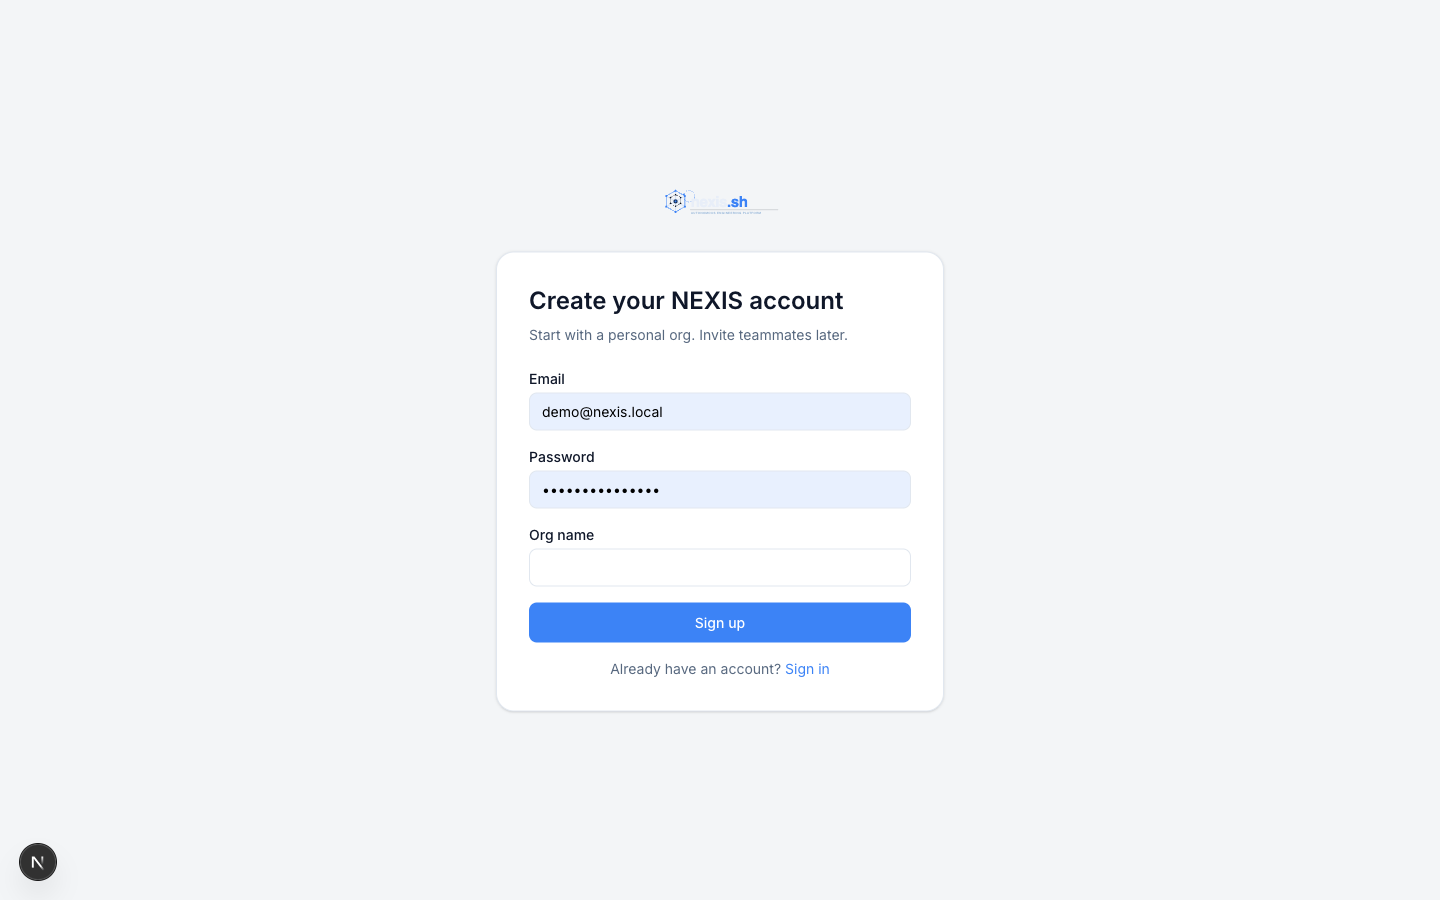
\includegraphics[width=0.85\textwidth]{../assets/screenshots/01-signup.png}
\caption{Sign-Up Screen ( new account registration ).}
\label{fig:signup}
\end{figure}

\begin{figure}[htbp]\centering
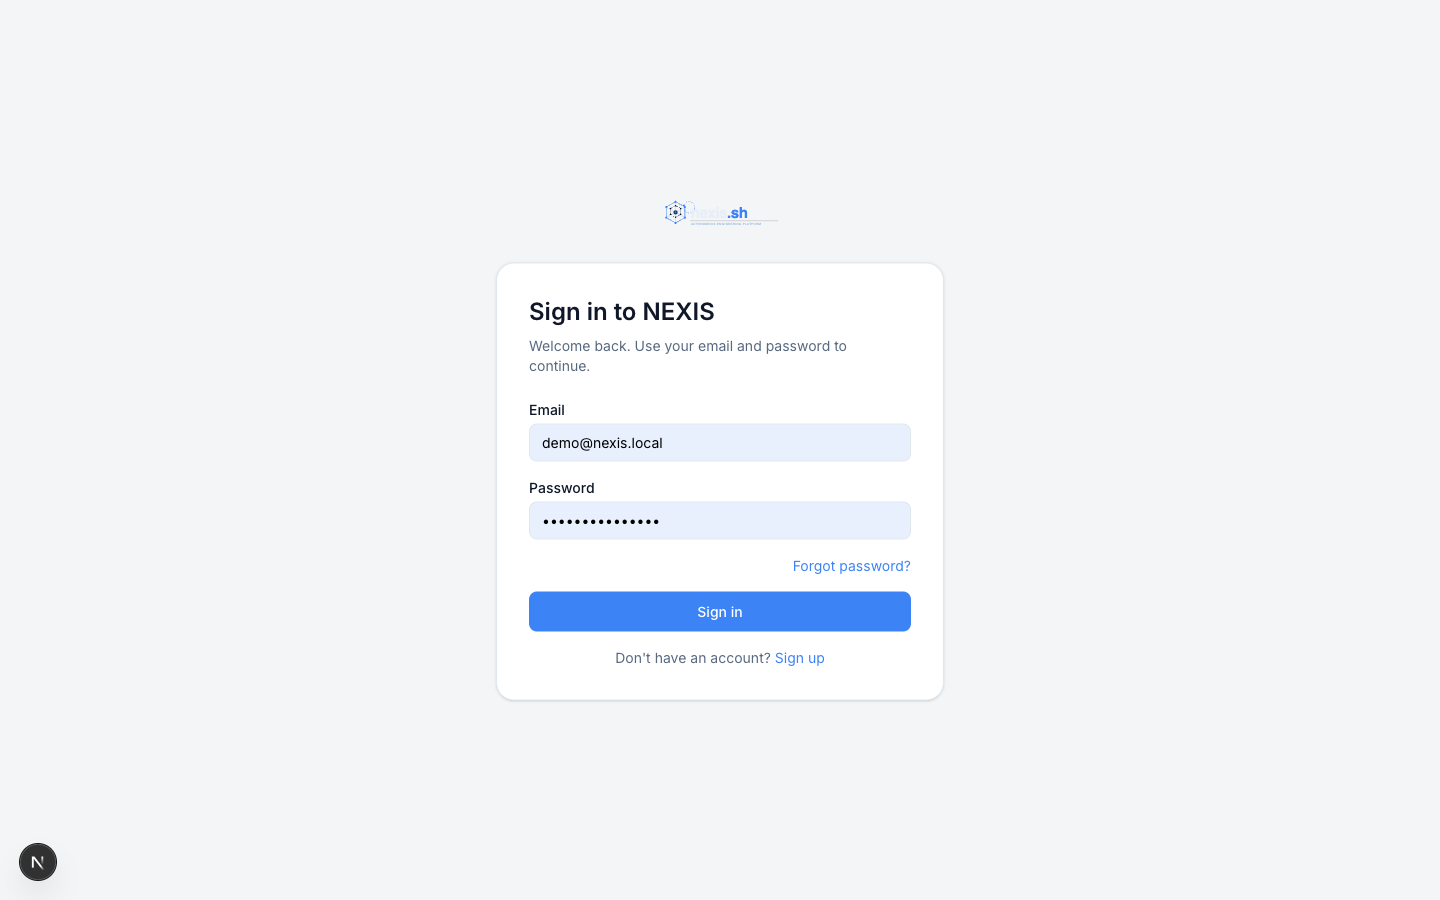
\includegraphics[width=0.85\textwidth]{../assets/screenshots/02-signin.png}
\caption{Sign-In Screen ( JWT session login with HttpOnly cookie ).}
\label{fig:signin}
\end{figure}

\begin{figure}[htbp]\centering
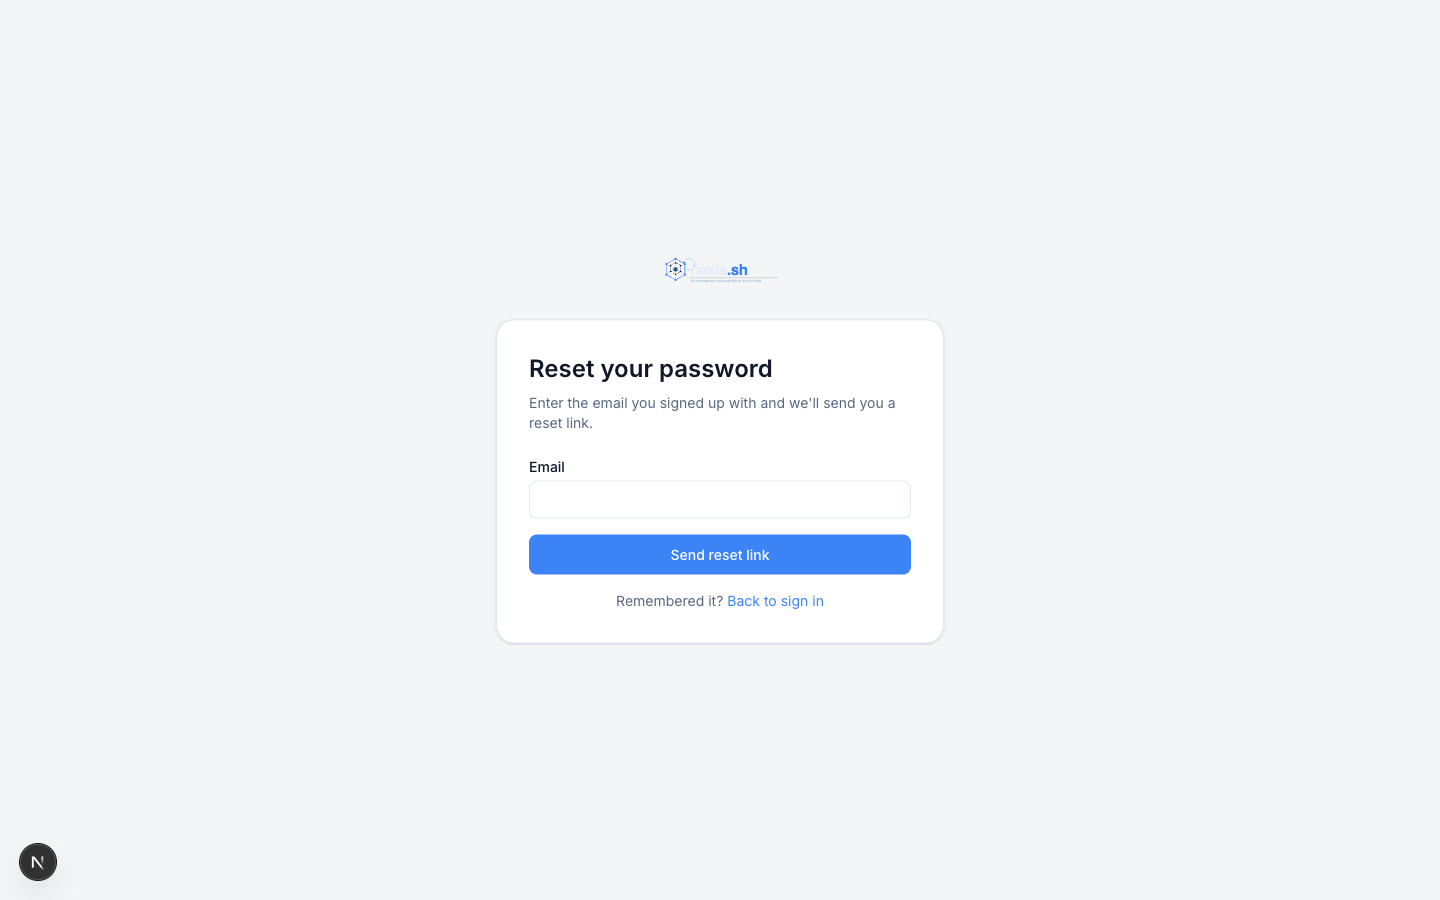
\includegraphics[width=0.85\textwidth]{../assets/screenshots/03-forgot-password.png}
\caption{Forgot-Password Screen ( non-leaky password-reset request ).}
\label{fig:forgot}
\end{figure}

\subsection{Admin / Owner Console}

The console home (Figure~\ref{fig:dashboard}) presents the organisation's
operational state at a glance: KPI tiles for MTTR, recovery success rate,
open incidents and mean tokens per run, an incidents-over-time chart, a
system status panel, a projects health grid, and a recent activity feed.

\begin{figure}[htbp]\centering
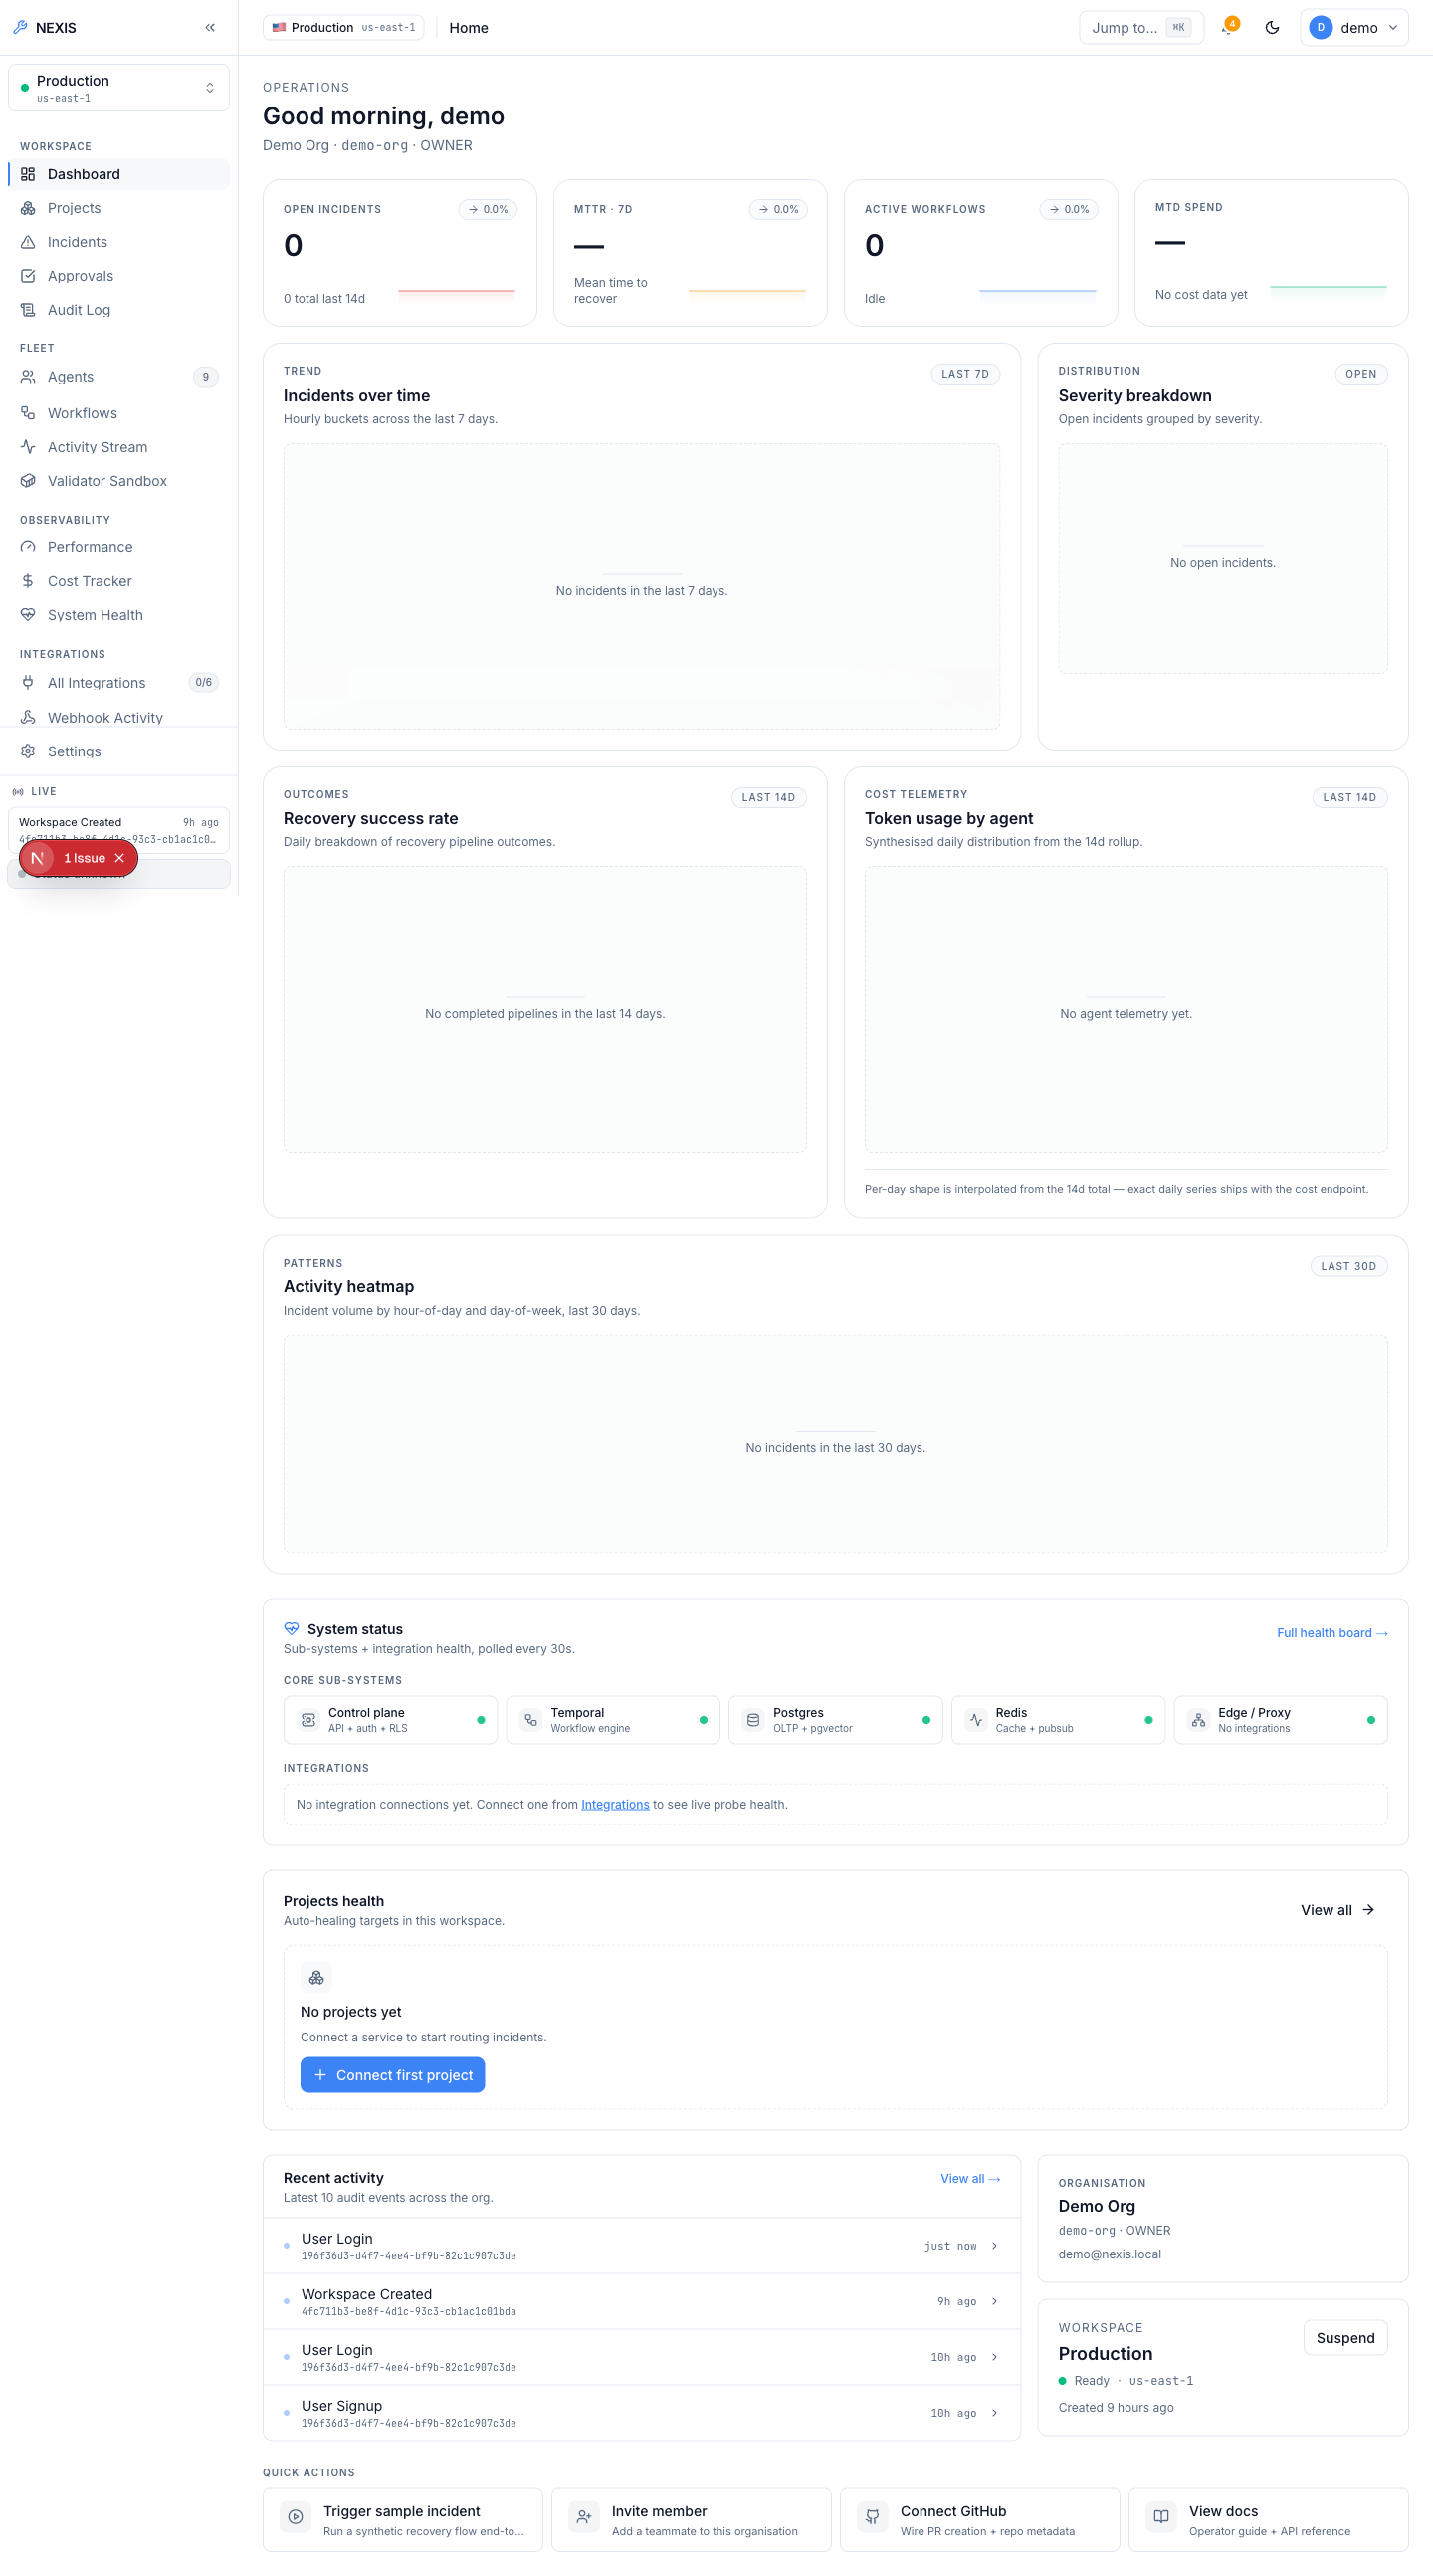
\includegraphics[width=0.85\textwidth]{../assets/screenshots/04-dashboard.png}
\caption{Admin Dashboard ( KPI tiles, incidents-over-time chart, and system status panel ).}
\label{fig:dashboard}
\end{figure}

The Agents page (Figure~\ref{fig:agents}) lists the full nine-agent fleet
across both layers --- the five Execution Team agents (Architect, Backend,
QA, DevOps, Data Engineer) and the Self-Healing Loop agents (Sentinel,
Pathfinder, Synthesiser, Validator) --- with each agent's role and status.

\begin{figure}[htbp]\centering
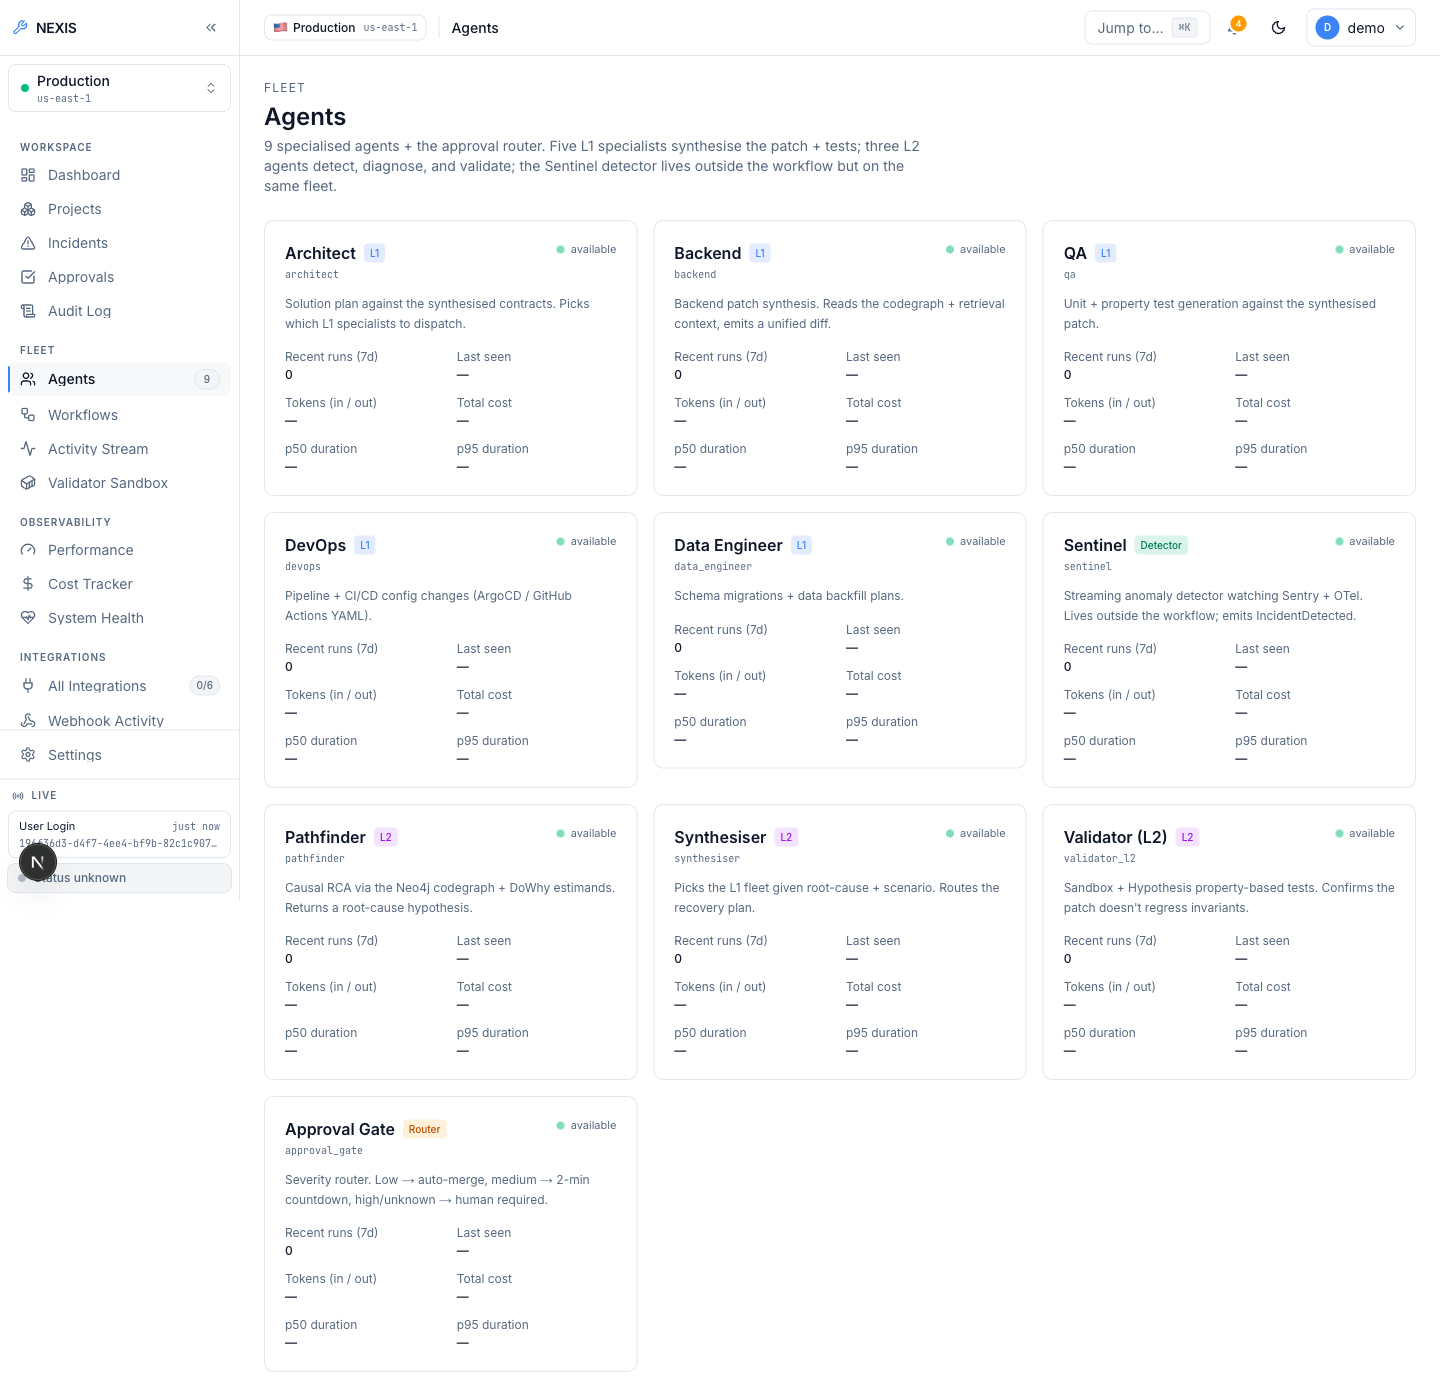
\includegraphics[width=0.85\textwidth]{../assets/screenshots/05-agents.png}
\caption{Agents Screen ( the nine-agent fleet roster across both layers ).}
\label{fig:agents}
\end{figure}

The Workflows page (Figure~\ref{fig:workflows}) lists RecoveryPipeline
executions; the Activity Stream (Figure~\ref{fig:activity}) is the
org-wide live event feed; and the Validator Sandbox console page
(Figure~\ref{fig:sandbox}) surfaces the Docker-sandboxed shadow-execution
service in which every candidate patch is run against its QA-generated
property tests before it may reach the approval gate.

\begin{figure}[htbp]\centering
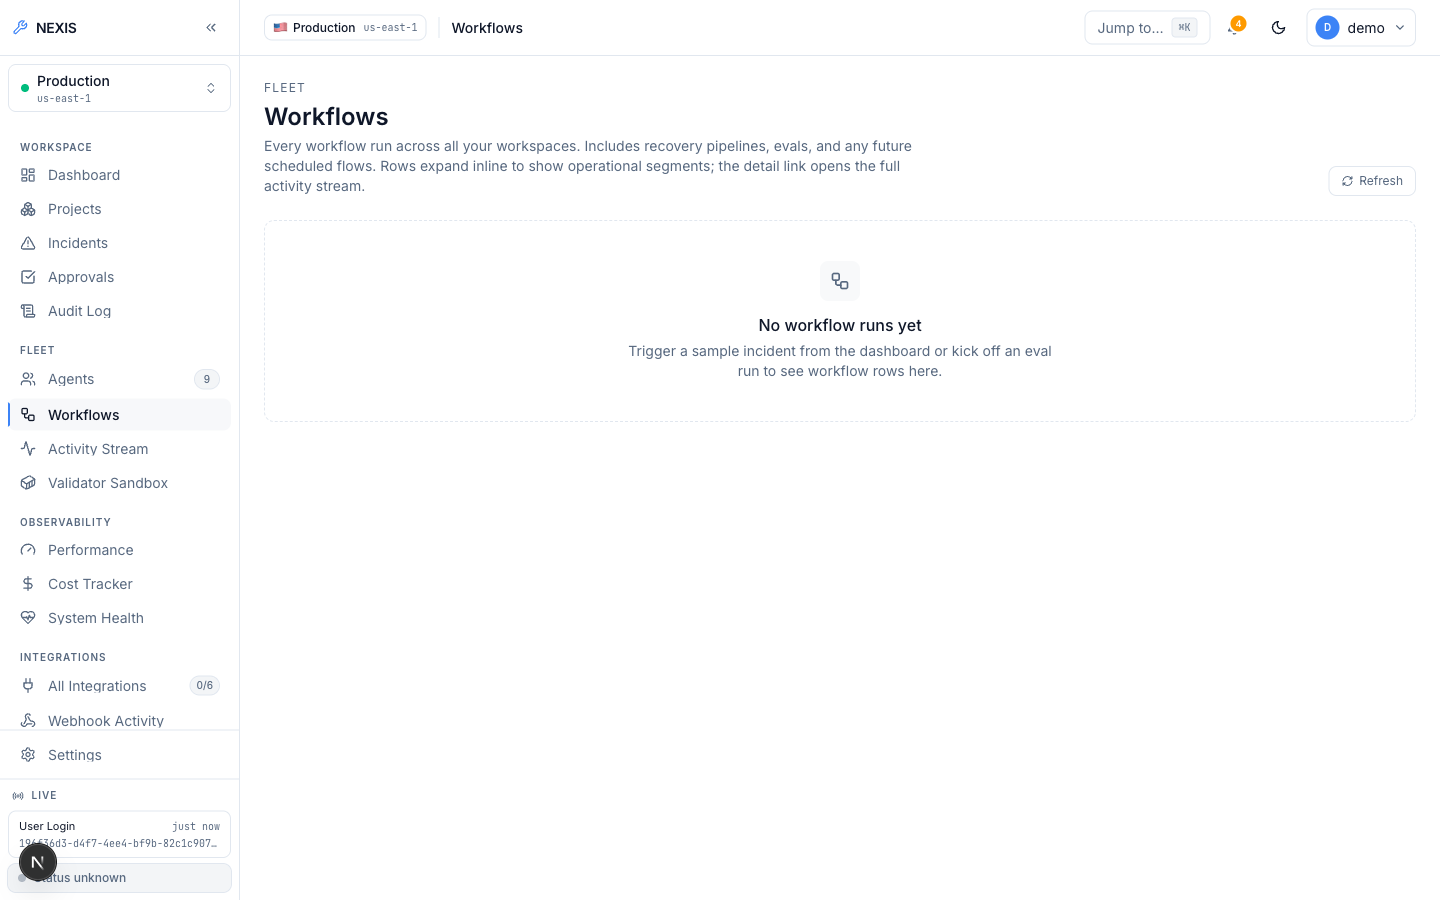
\includegraphics[width=0.85\textwidth]{../assets/screenshots/06-workflows.png}
\caption{Workflows Screen ( RecoveryPipeline run listing ).}
\label{fig:workflows}
\end{figure}

\begin{figure}[htbp]\centering
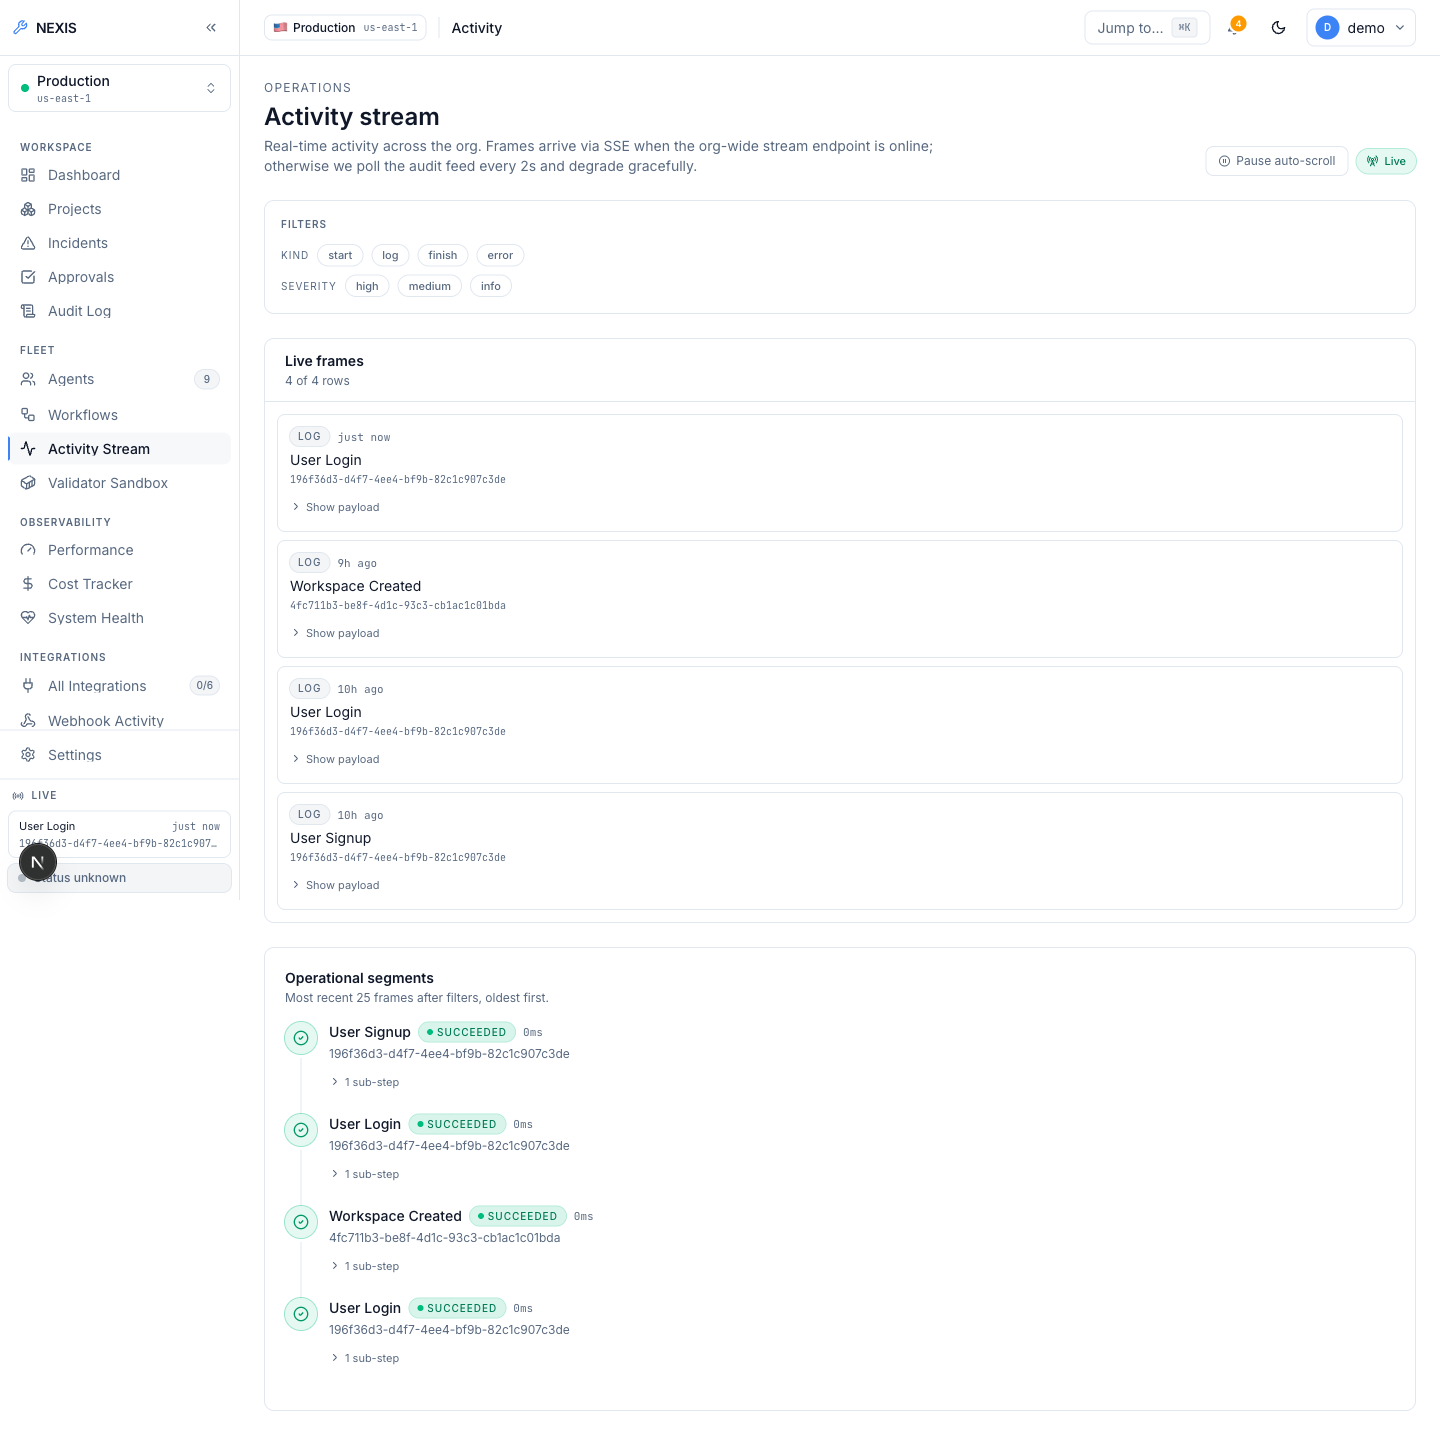
\includegraphics[width=0.85\textwidth]{../assets/screenshots/07-activity-stream.png}
\caption{Activity Stream ( organisation-wide live event feed ).}
\label{fig:activity}
\end{figure}

\begin{figure}[htbp]\centering
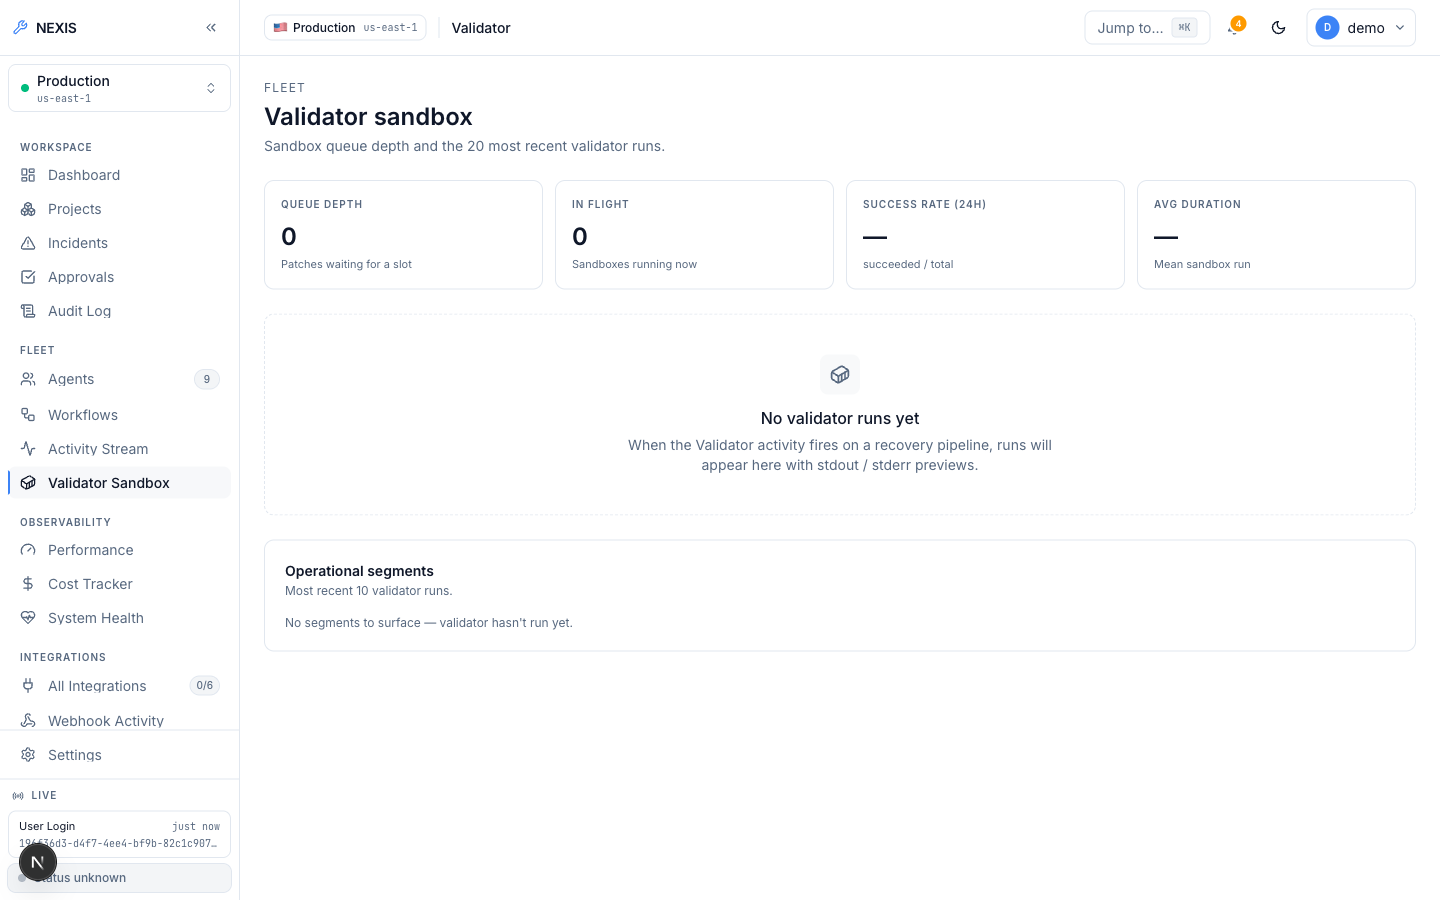
\includegraphics[width=0.85\textwidth]{../assets/screenshots/08-validator-sandbox.png}
\caption{Validator Sandbox Console ( sandboxed shadow execution of candidate patches ).}
\label{fig:sandbox}
\end{figure}

The Audit Log (Figure~\ref{fig:audit}) is append-only and hash-chained: each
entry incorporates the hash of its predecessor, so any tampering with a past
row breaks the chain and is detectable by the cryptographic verify endpoint.
The log supports CSV export for offline review.

\begin{figure}[htbp]\centering
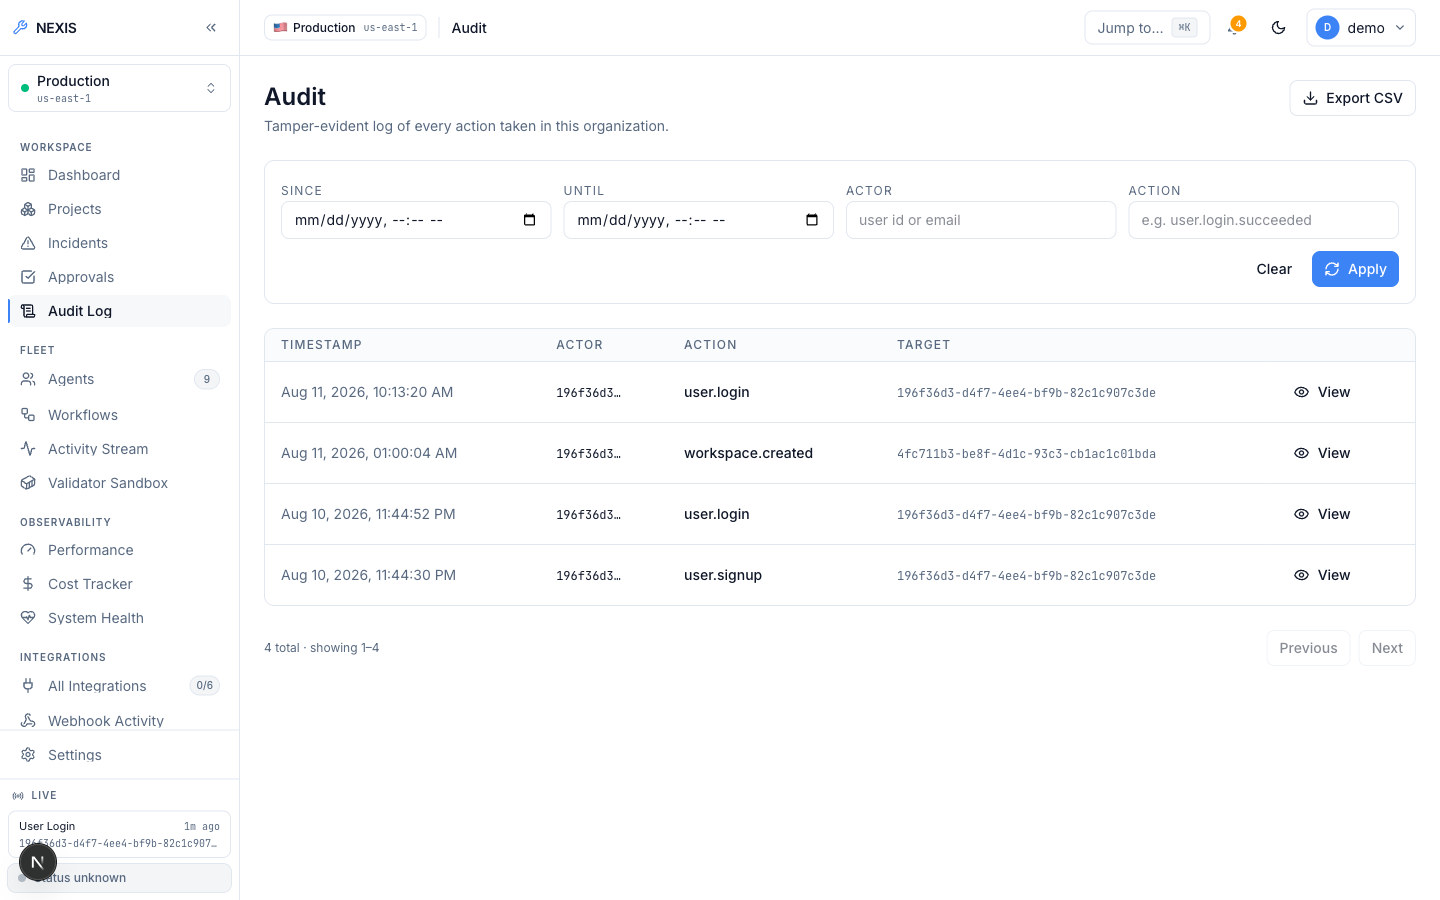
\includegraphics[width=0.85\textwidth]{../assets/screenshots/11-audit-log.png}
\caption{Audit Log ( append-only, hash-chained entries with CSV export ).}
\label{fig:audit}
\end{figure}

\subsection{Members, Roles, and Sessions}

The Members settings page (Figure~\ref{fig:members}) lists the
organisation's members with their roles (owner, admin, member) and exposes
the intelligent role-recommendation panel. This panel is backed by the real
heuristic engine described in Chapter~4, not a mock: it evaluates concrete
signals already captured in the schema --- a member with five or more
admin-gated audit-log actions in 30 days who is not yet an admin, an admin
with no login in 90 or more days, and an active admin with zero admin-gated
actions --- and each recommendation carries a plain-language rationale
naming the specific evidence numbers behind it. An admin can accept the
recommendation (applying the role change under an optimistic-concurrency
guard) or dismiss it, which starts a 30-day per-rule cool-down.

\begin{figure}[htbp]\centering
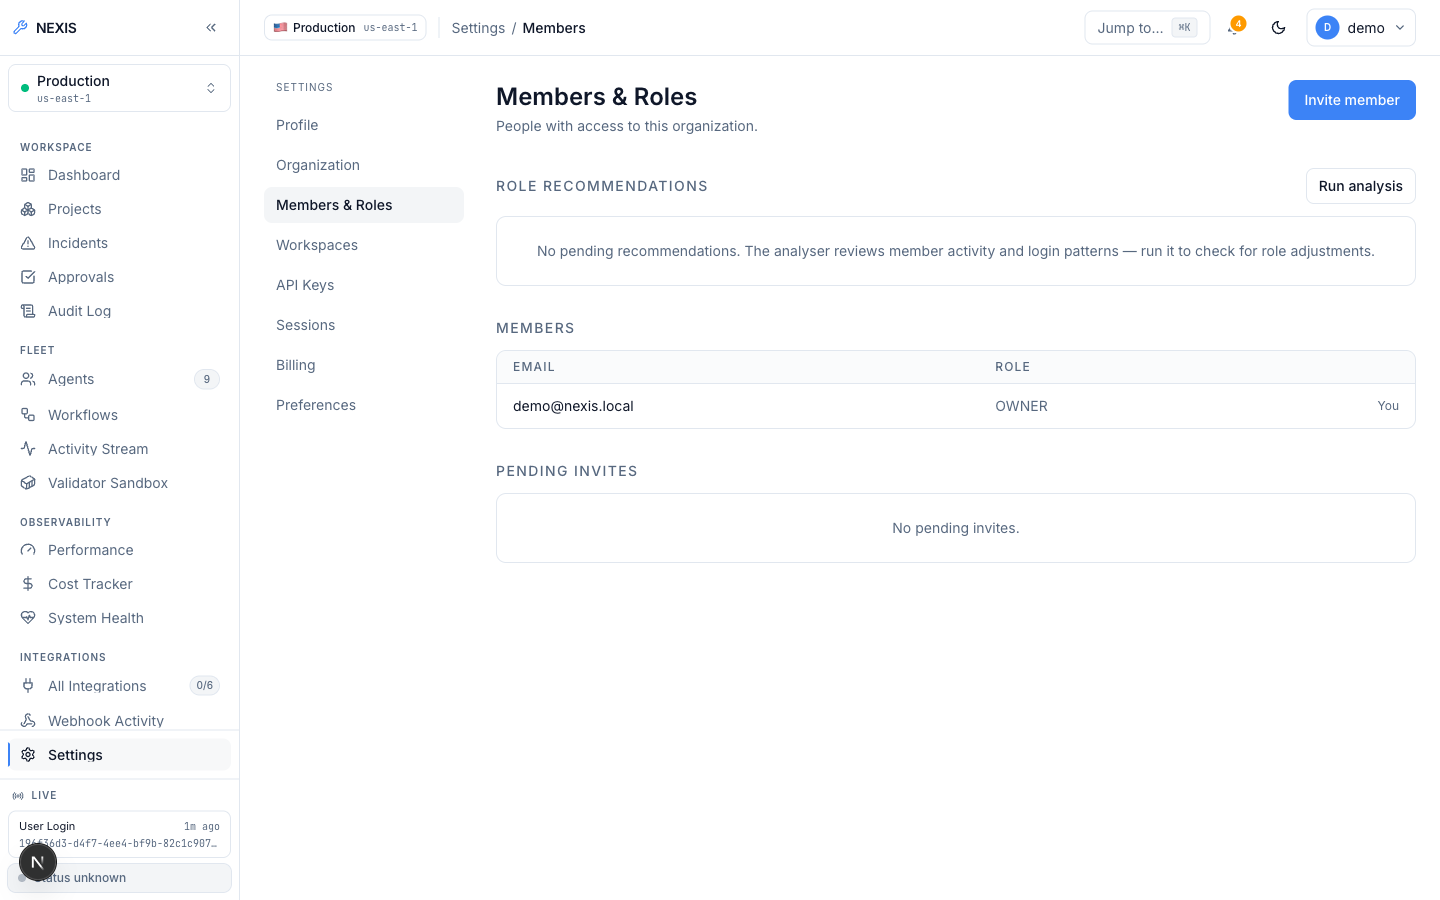
\includegraphics[width=0.85\textwidth]{../assets/screenshots/13-settings-members.png}
\caption{Members Settings ( members list with the heuristic role-recommendation panel ).}
\label{fig:members}
\end{figure}

Session management (Figure~\ref{fig:sessions}) lists every active session
with its device, IP address, user agent, and last-seen time; any session can
be revoked remotely, and the caller's own session is marked with a ``This
device'' badge. API keys (Figure~\ref{fig:apikeys}) are scoped bearer tokens
(\code{nx\_live\_...}) that can be created, listed, and revoked. Billing
(Figure~\ref{fig:billing}) surfaces Stripe~\cite{stripe} usage and payment
method management, and the Organization page (Figure~\ref{fig:orgsettings})
holds organisation-level profile settings.

\begin{figure}[htbp]\centering
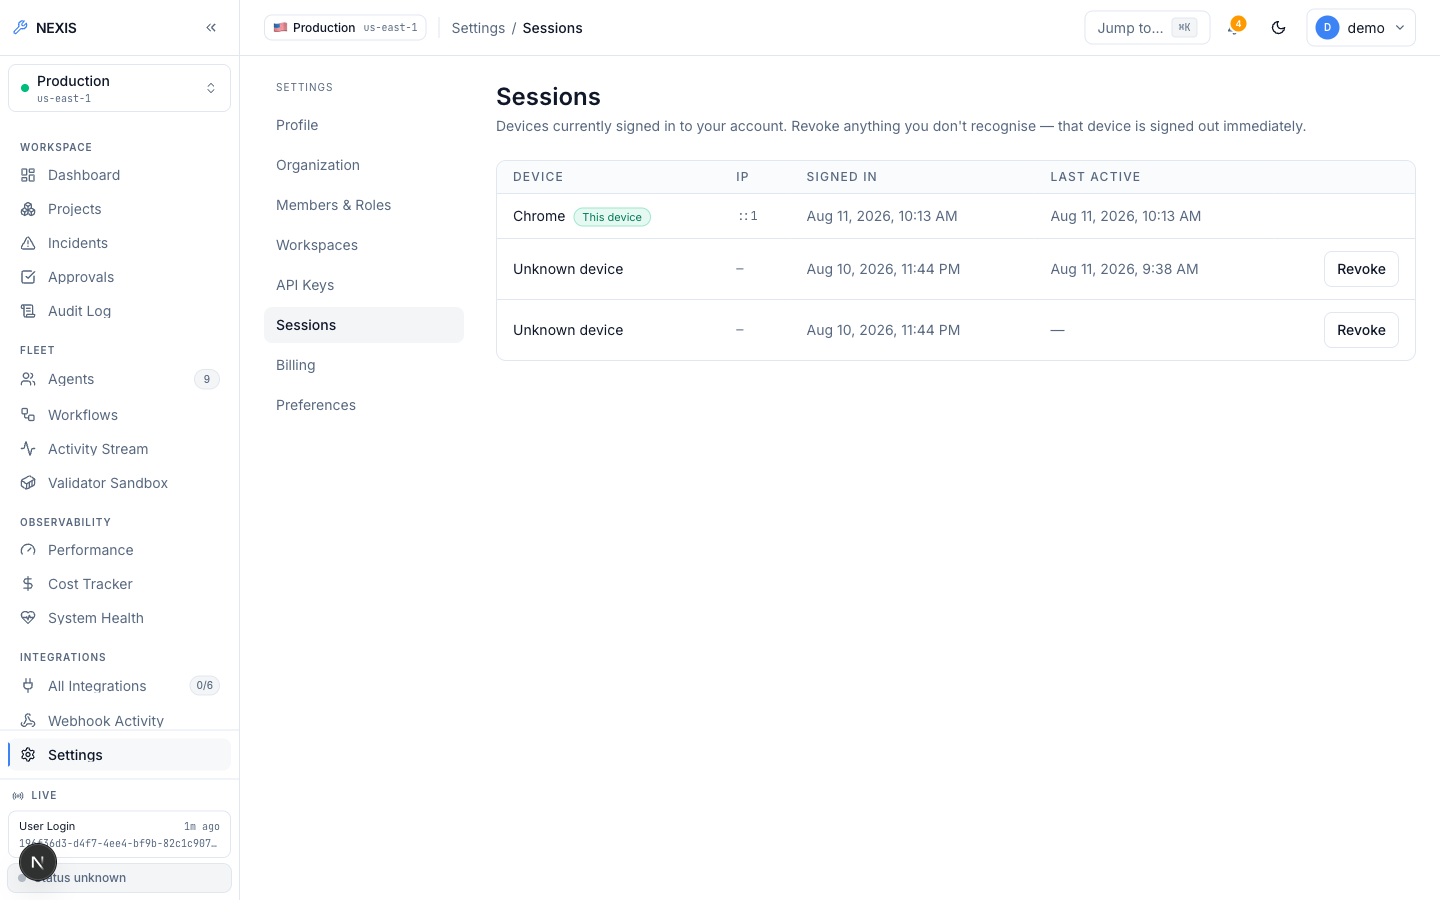
\includegraphics[width=0.85\textwidth]{../assets/screenshots/14-settings-sessions.png}
\caption{Sessions Settings ( active sessions with device, IP, and remote revoke ).}
\label{fig:sessions}
\end{figure}

\begin{figure}[htbp]\centering
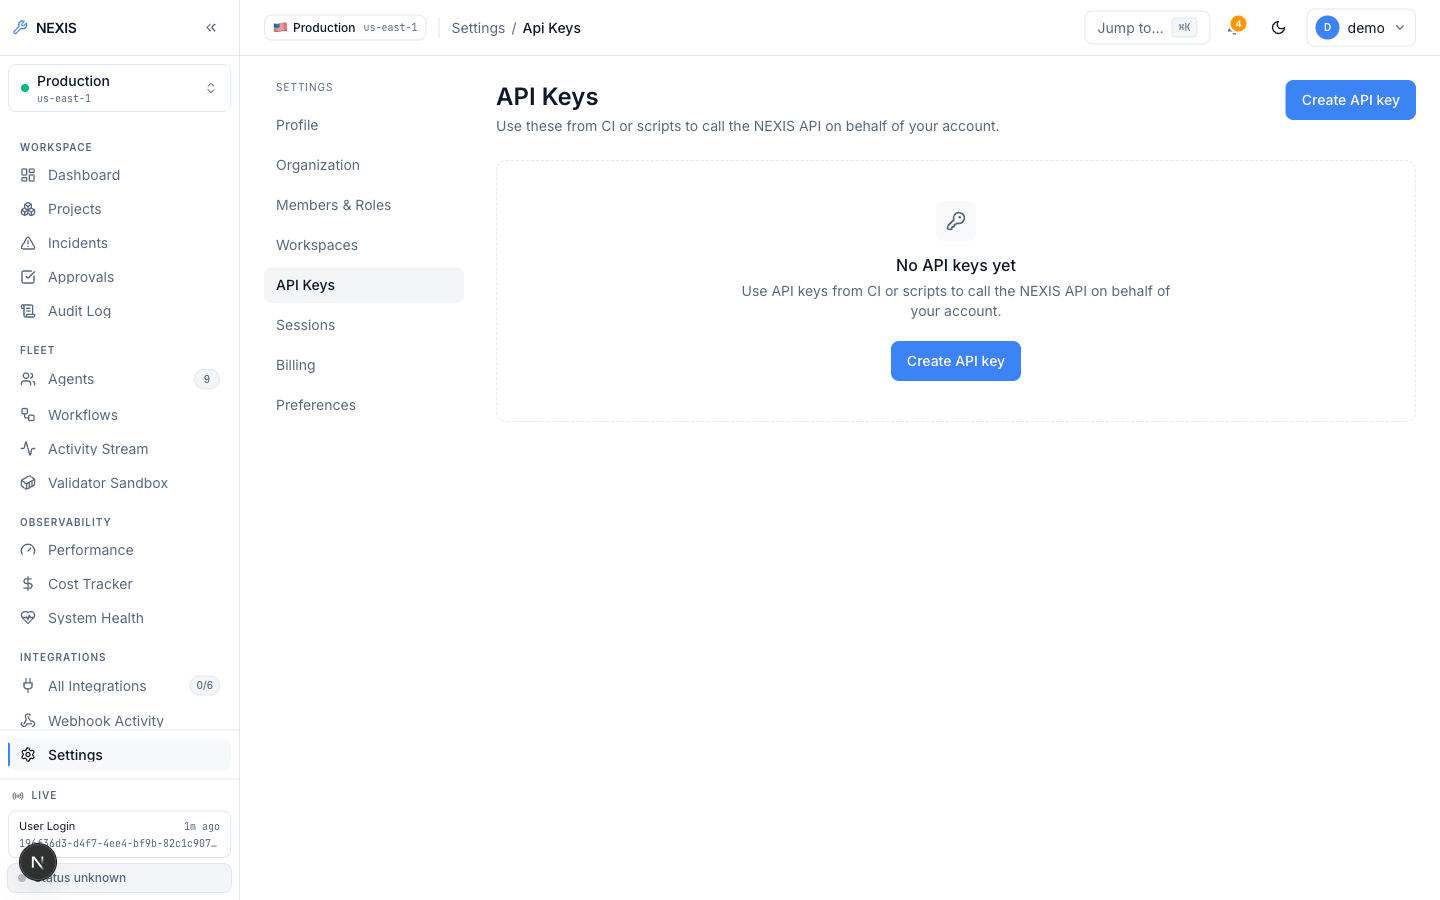
\includegraphics[width=0.85\textwidth]{../assets/screenshots/15-settings-apikeys.png}
\caption{API Keys Settings ( scoped bearer key creation, listing, and revocation ).}
\label{fig:apikeys}
\end{figure}

\begin{figure}[htbp]\centering
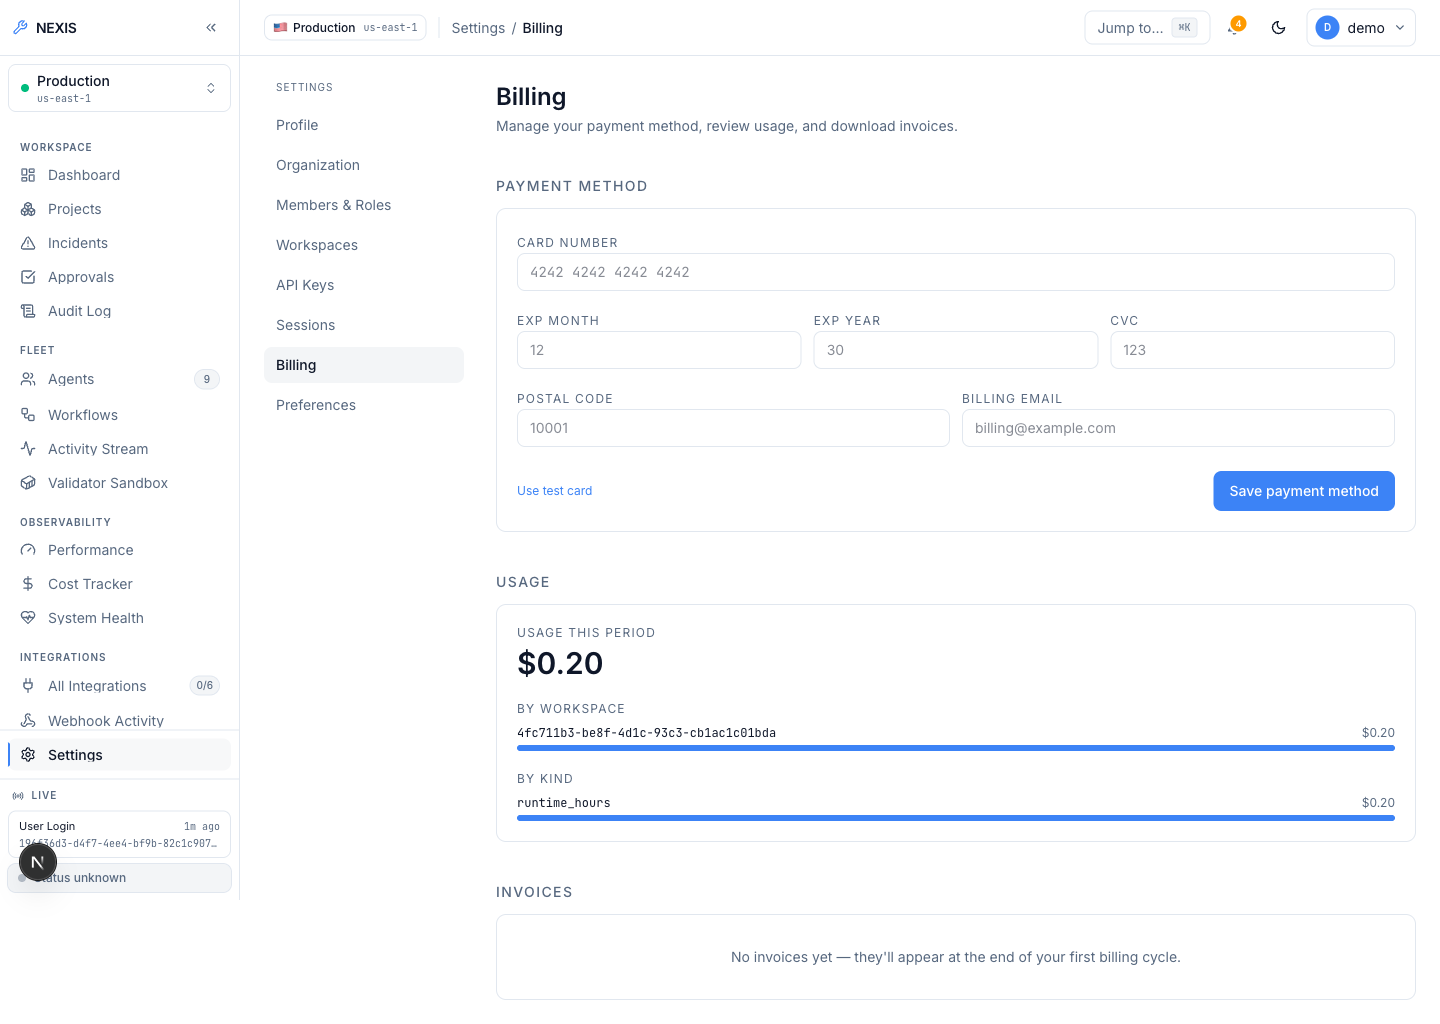
\includegraphics[width=0.85\textwidth]{../assets/screenshots/16-settings-billing.png}
\caption{Billing Settings ( Stripe usage and payment-method management ).}
\label{fig:billing}
\end{figure}

\begin{figure}[htbp]\centering
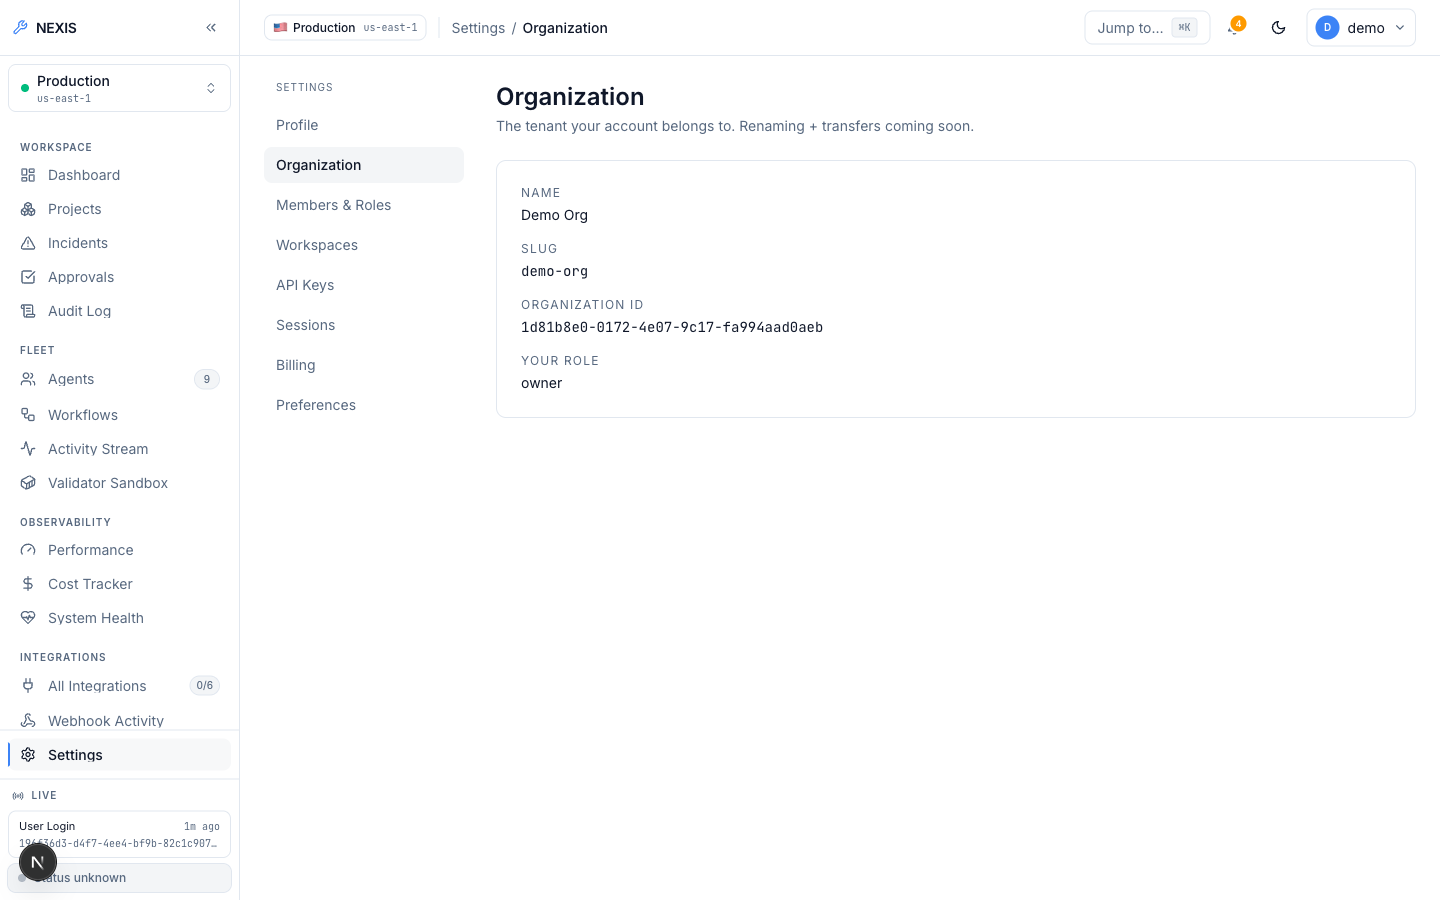
\includegraphics[width=0.85\textwidth]{../assets/screenshots/17-settings-organization.png}
\caption{Organization Settings ( organisation profile management ).}
\label{fig:orgsettings}
\end{figure}

\subsection{Self-Healing Loop --- Live Evidence}
\label{sec:liveevidence}

This subsection is the evidentiary core of the report. It documents two real,
complete, end-to-end executions of the nine-agent RecoveryPipeline against a
live local LLM (Ollama, \code{qwen2.5-coder:14b} and \code{gpt-oss:20b}) ---
one run that timed out at the human approval gate and was safely
auto-rejected, and one run that was approved within the window and succeeded
fully. Both outcomes are shown exactly as they occurred.

The entry point is the Live Demo console (Figure~\ref{fig:livedemo}), which
presents 27 curated fault-scenario cards drawn from a broader fixture
taxonomy spanning application, database, deploy, observability, and security
categories. To be precise about the current state: exactly one of the 27
scenarios is fully wired end-to-end today; the remaining cards are
UI-complete but backend-pending and are labelled ``Coming soon'' in the
interface. The runs documented below were triggered through the wired path.

\begin{figure}[htbp]\centering
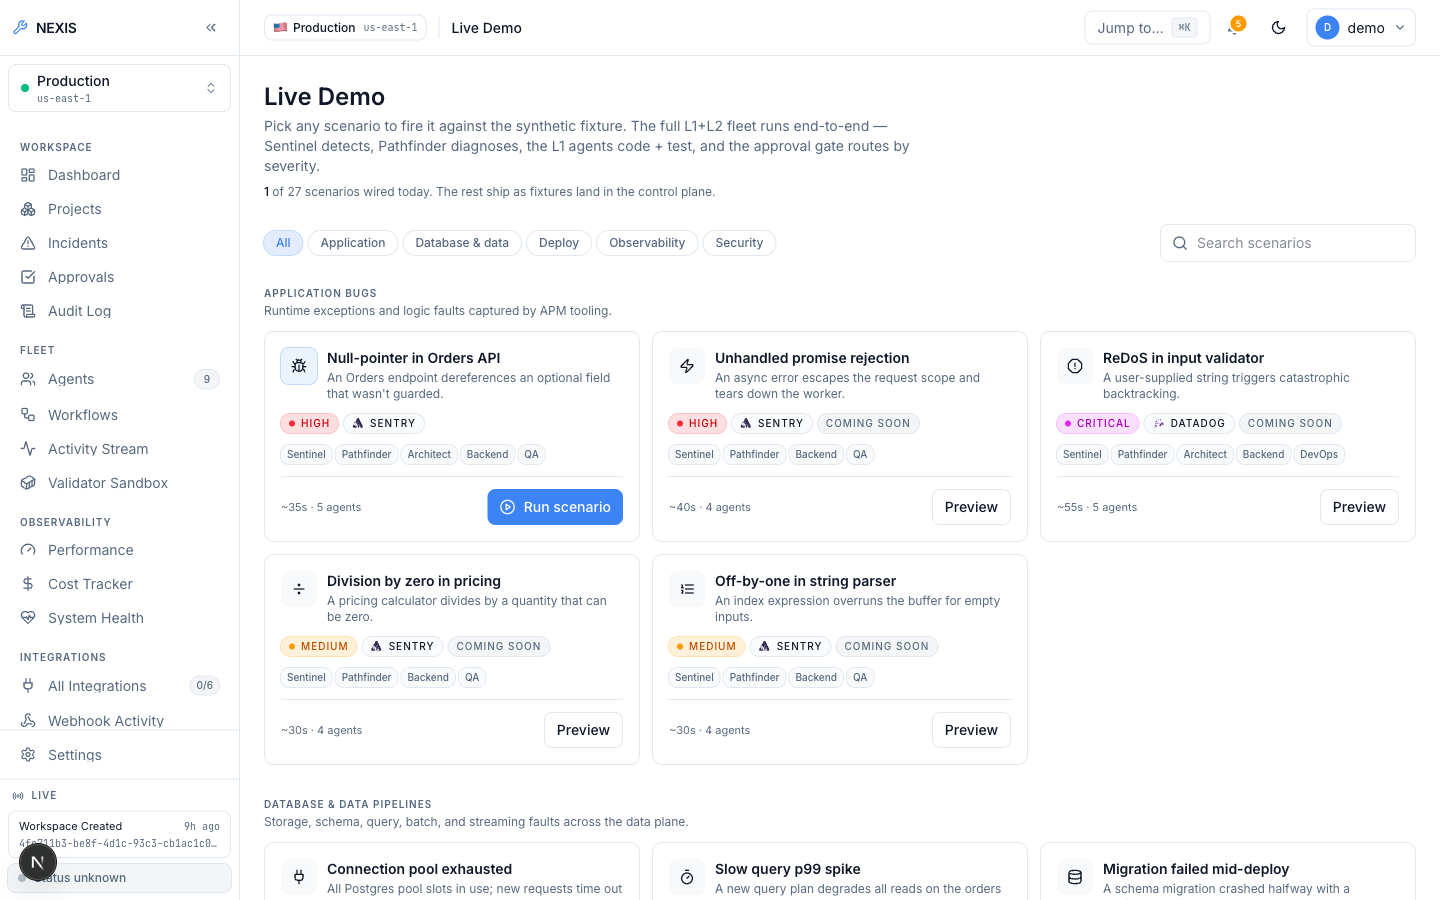
\includegraphics[width=0.85\textwidth]{../assets/screenshots/26-live-demo.png}
\caption{Live Demo Console ( 27-scenario fault-injection picker; one scenario fully wired, the rest backend-pending ).}
\label{fig:livedemo}
\end{figure}

Figure~\ref{fig:livemid} captures the first run genuinely mid-flight. The
Architect, Backend, and QA steps have already completed --- each showing a
real, non-zero token count and cost figure accumulated from actual LLM
calls --- while the DevOps and Data Engineer steps are executing in
parallel. These visible token and cost figures are themselves evidence: a
stubbed or templated pipeline would report zero tokens, whereas every
completed step here carries the token consumption of the model call that
produced its output.

\begin{figure}[htbp]\centering
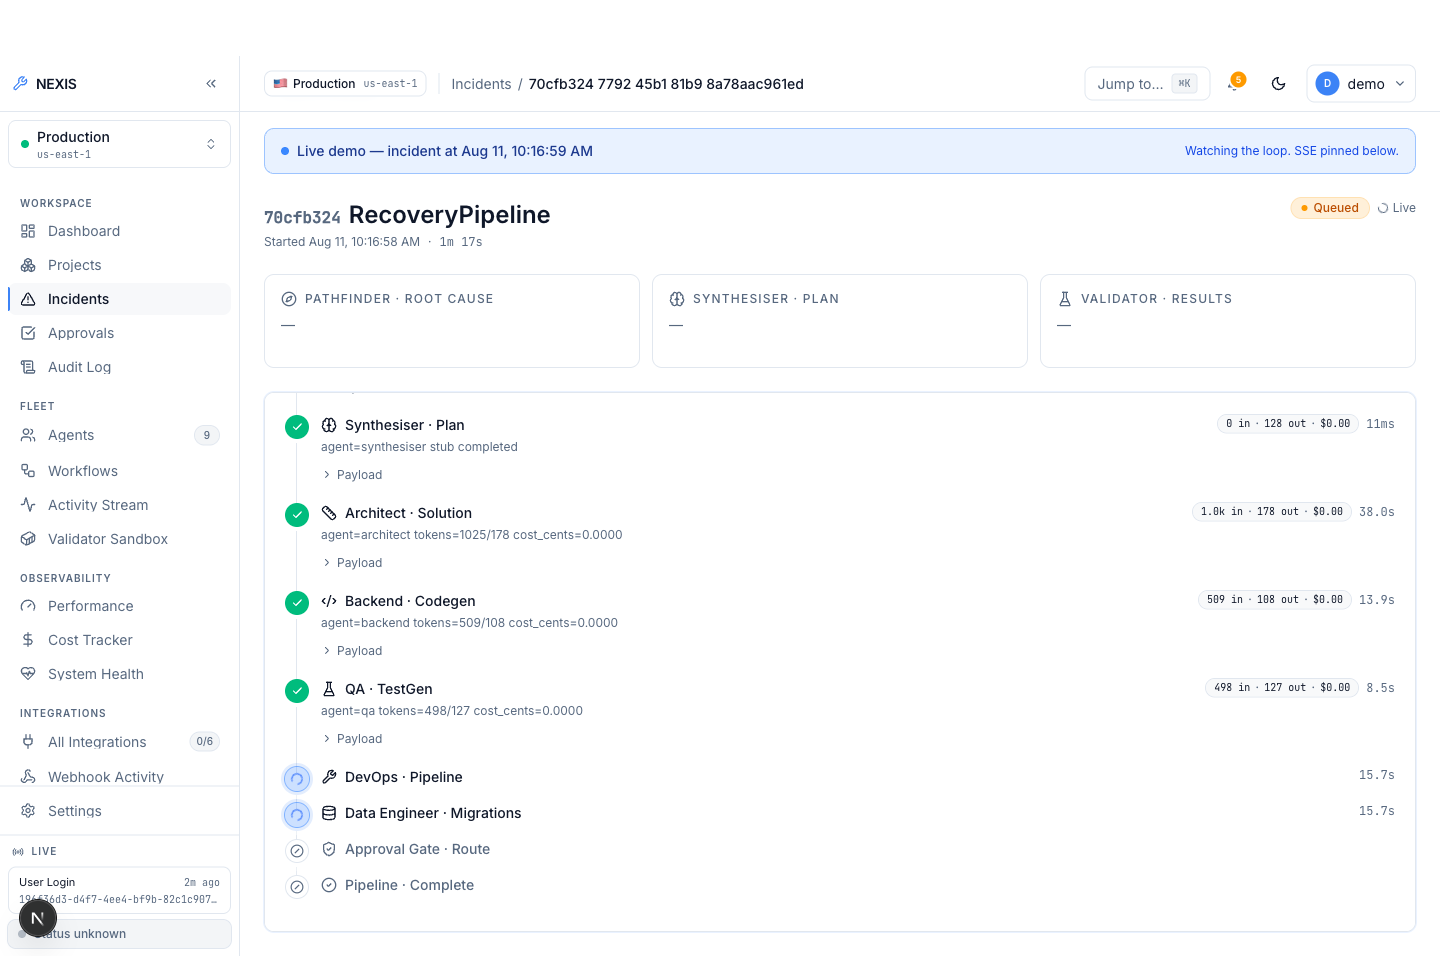
\includegraphics[width=0.85\textwidth]{../assets/screenshots/35-incident-live-progress.png}
\caption{Incident Detail, Mid-Flight ( live pipeline with completed Architect/Backend/QA steps showing real token counts; DevOps and Data Engineer running in parallel ).}
\label{fig:livemid}
\end{figure}

Figure~\ref{fig:livefinal} shows the same run moments later: every Layer-1
and Layer-2 step has completed green --- the patch has been generated,
property-tested, and validated in the sandbox --- and the run now sits at
severity ``Medium'' with approval status ``Pending'', awaiting a human
decision inside the 120-second window.

\begin{figure}[htbp]\centering
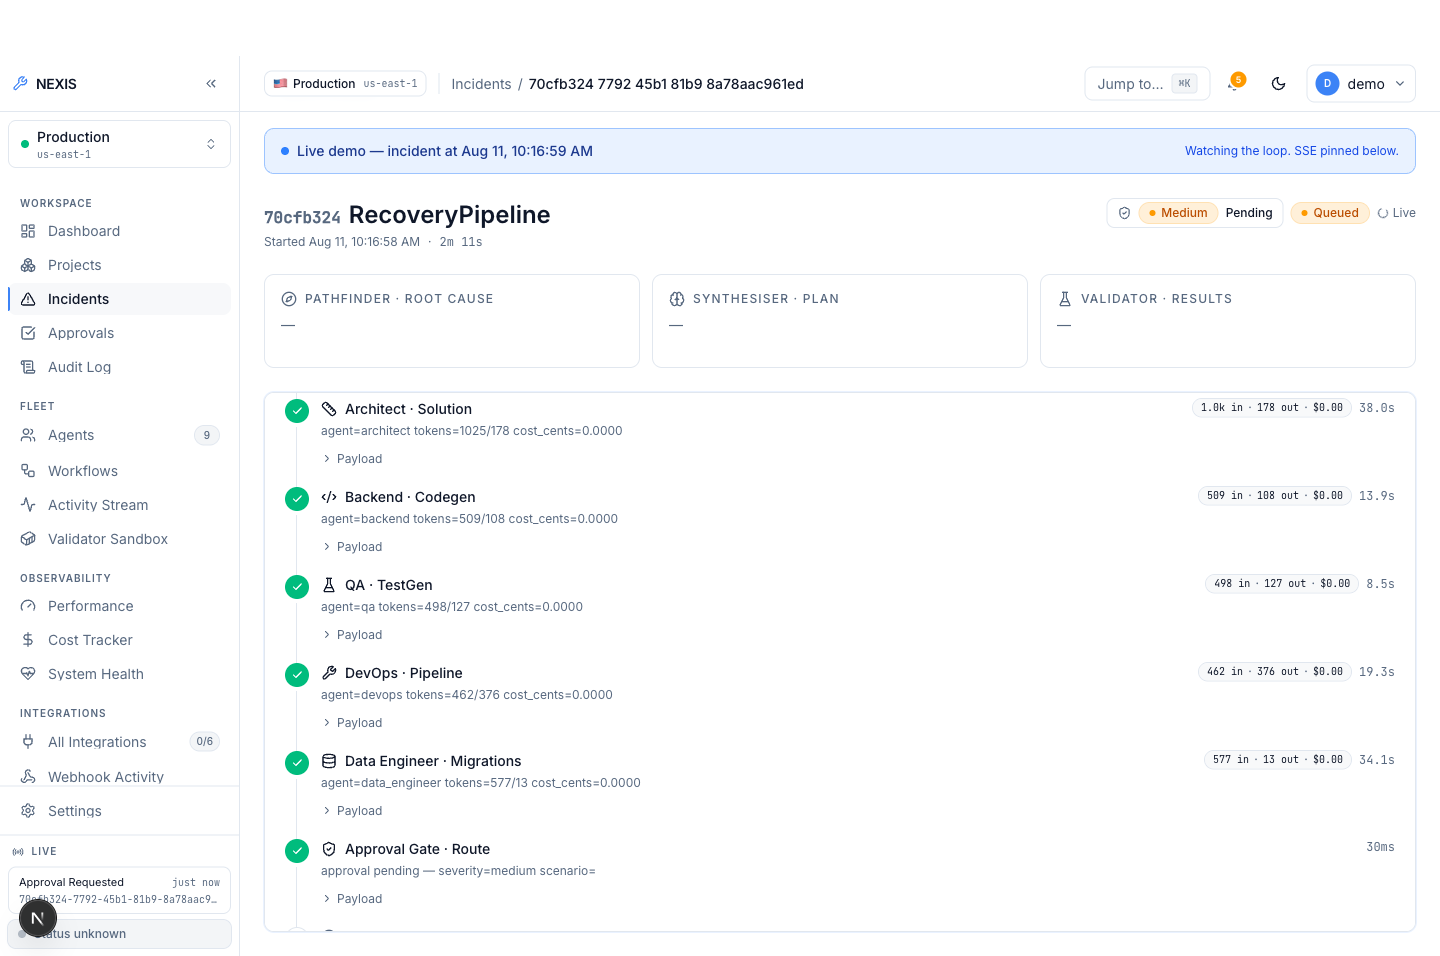
\includegraphics[width=0.85\textwidth]{../assets/screenshots/36-incident-live-final.png}
\caption{Incident Detail, Pipeline Complete ( all L1/L2 steps green; severity Medium, approval Pending ).}
\label{fig:livefinal}
\end{figure}

That pending state is reflected in the Approvals queue
(Figure~\ref{fig:approvals}): a real pending-approval row with the three
human decision actions --- Reject, Modify, and Approve.

\begin{figure}[htbp]\centering
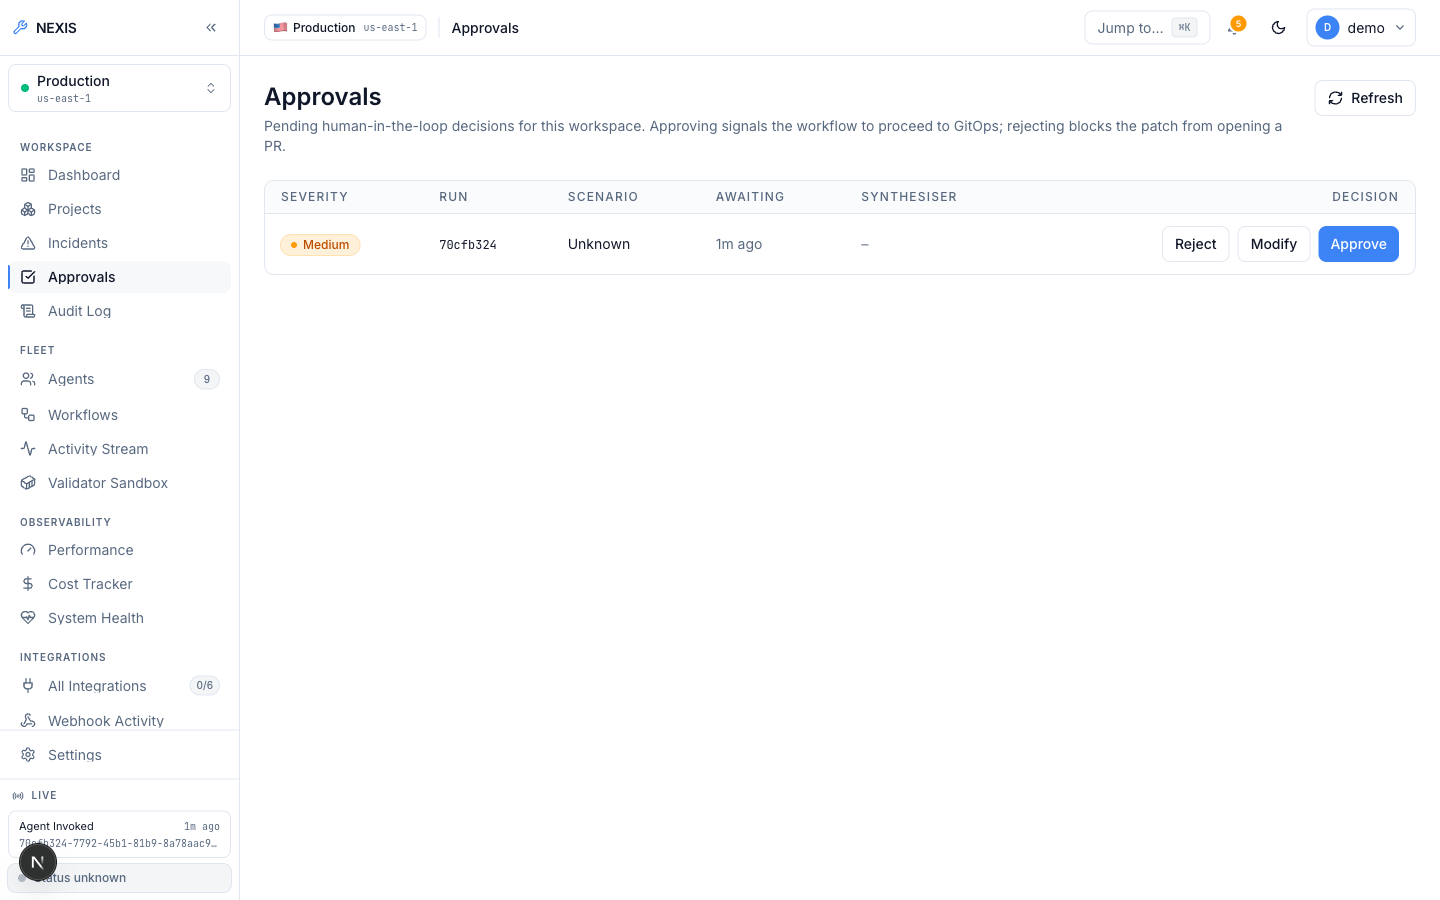
\includegraphics[width=0.85\textwidth]{../assets/screenshots/10-approvals.png}
\caption{Approvals Queue ( real pending approval row with Reject / Modify / Approve actions ).}
\label{fig:approvals}
\end{figure}

The Modify action opens the dialog in Figure~\ref{fig:modifydialog}. This is
the RLHF mechanism described in Chapter~4 made concrete: the engineer edits
the LLM-generated unified diff directly in the embedded editor before
approving, and the edited diff --- along with every other terminal approval
decision --- is persisted as a row in the \code{feedback\_examples} table.
Those rows feed a JSONL export endpoint intended for future fine-tuning;
actually submitting a paid fine-tuning job against the exported data is a
deliberate manual step, not an automated one.

\begin{figure}[htbp]\centering
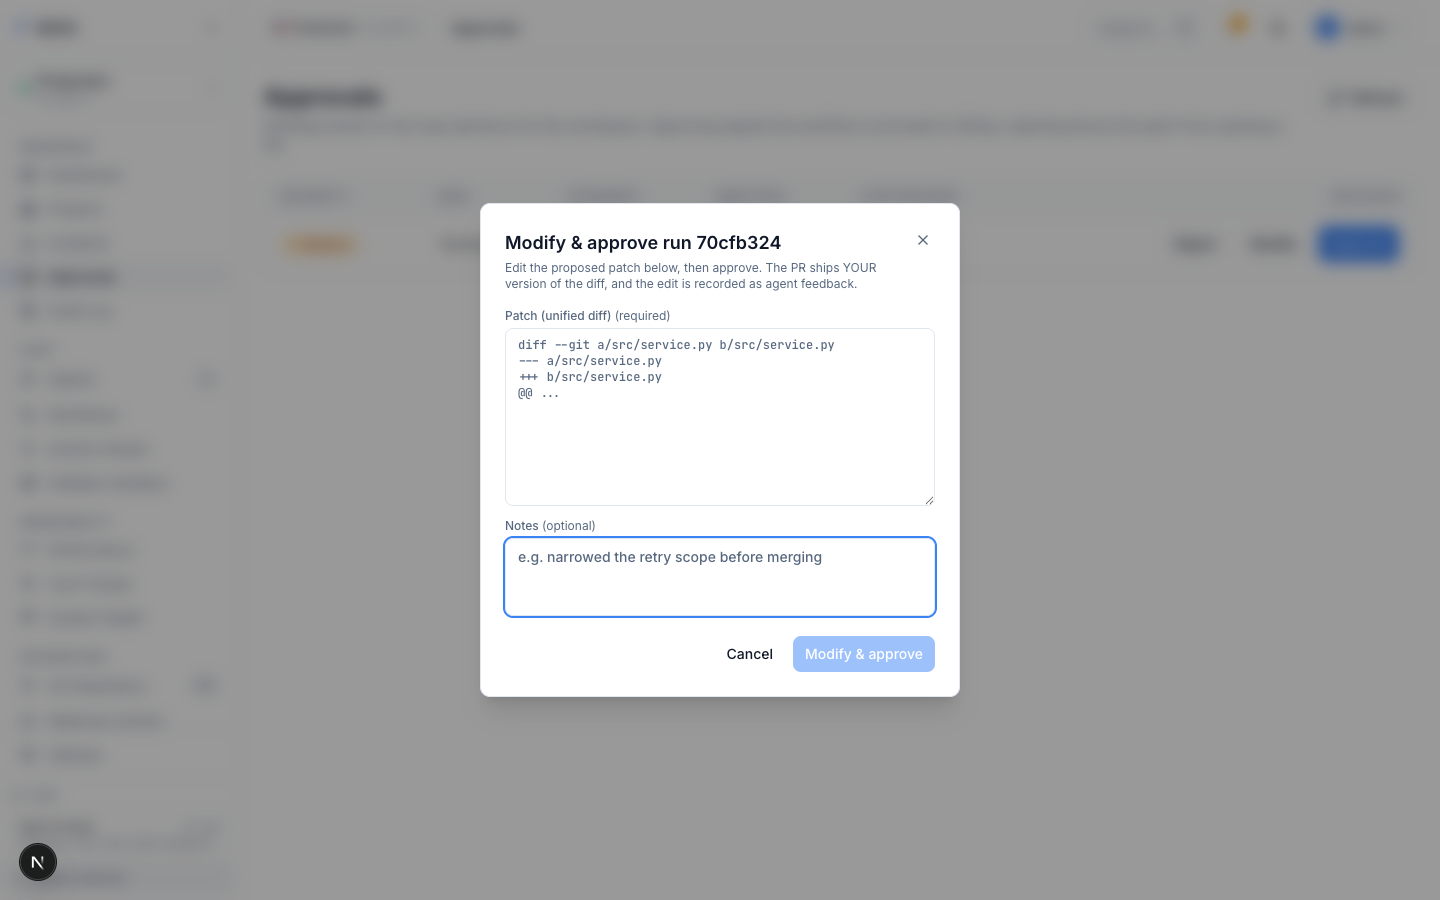
\includegraphics[width=0.85\textwidth]{../assets/screenshots/37-approval-modify-dialog.png}
\caption{Modify-and-Approve Dialog ( RLHF diff editing; the engineer's edit becomes a feedback\_examples training row ).}
\label{fig:modifydialog}
\end{figure}

Figure~\ref{fig:timeoutrun} is an honest negative result, reported
deliberately. For this first run, the 120-second approval window elapsed
before a decision was recorded, and the workflow terminated the run as
\code{timeout\_rejected}. This is the timeout safety mechanism working
exactly as designed: when no human decision arrives in time, the system's
default is to refuse to deploy unreviewed code, not to proceed. A pipeline
that silently auto-deployed on timeout would be a defect; this behaviour is
the intended safe failure mode.

\begin{figure}[htbp]\centering
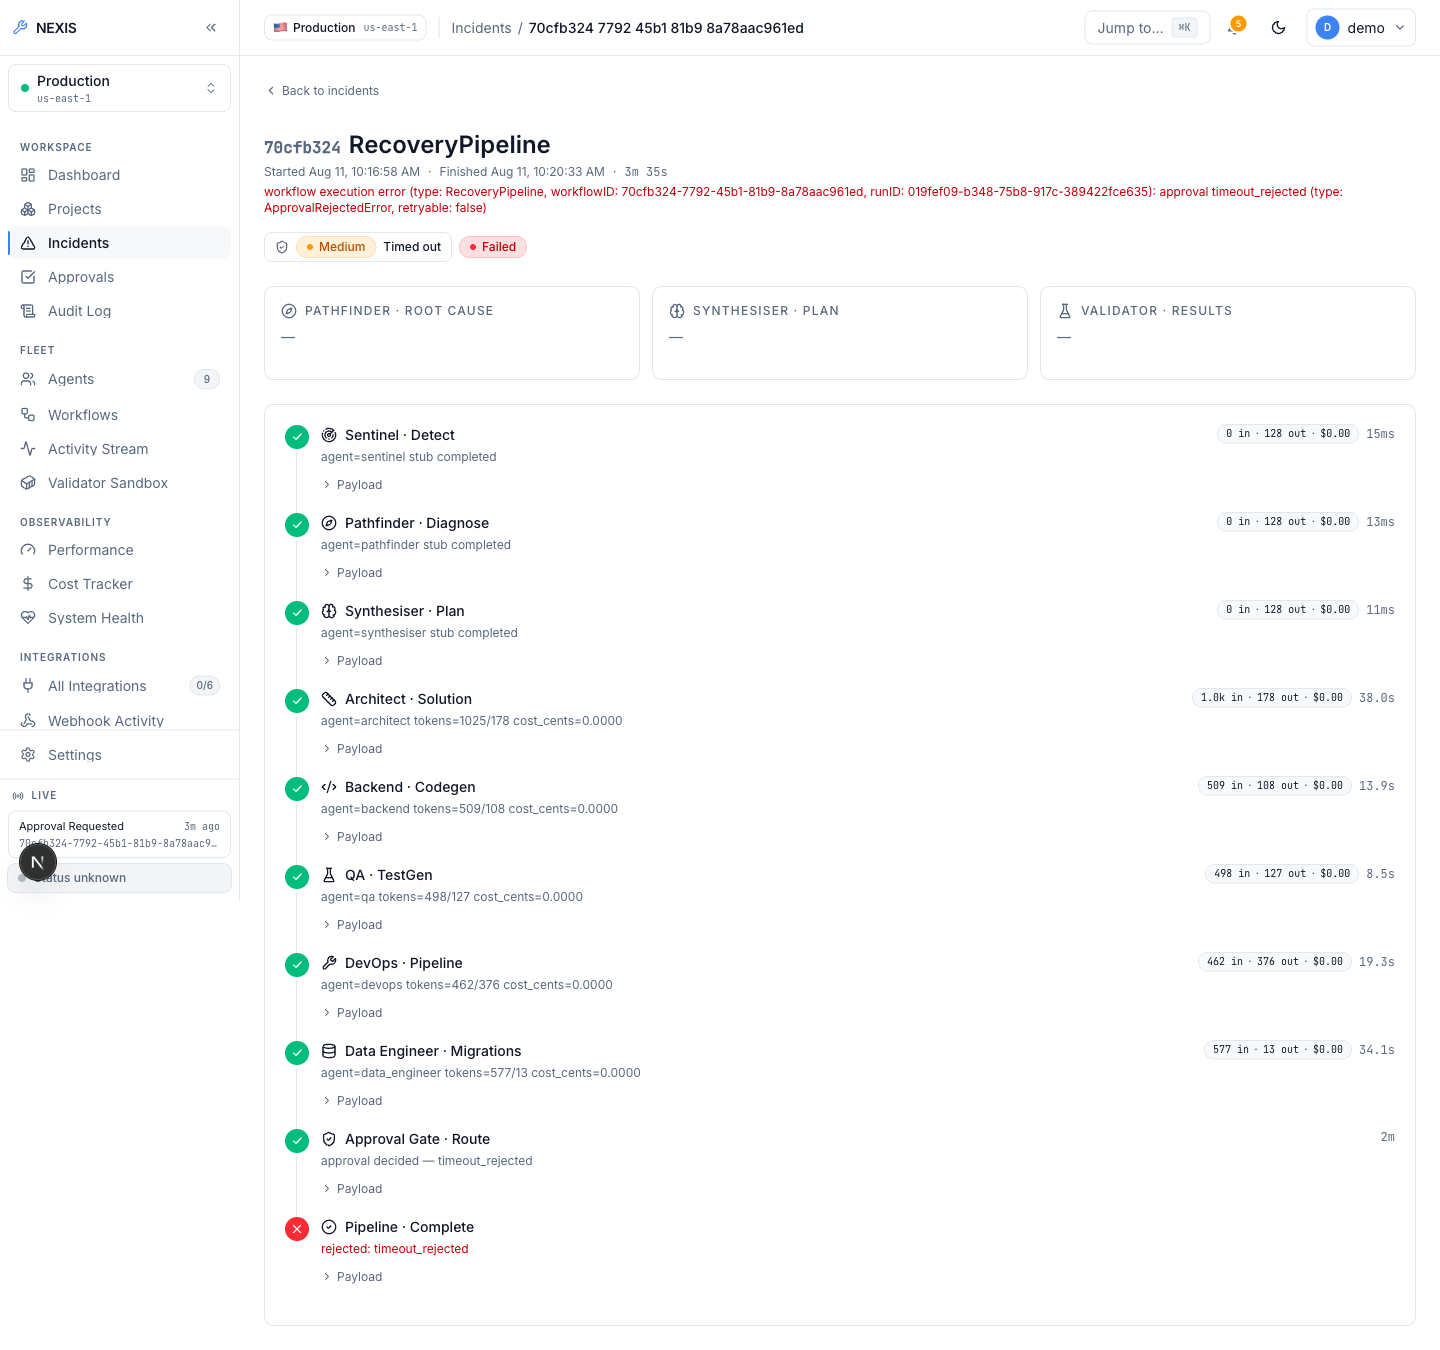
\includegraphics[width=0.85\textwidth]{../assets/screenshots/39-incident-approved-final.png}
\caption{Timeout-Rejected Run ( the 120-second approval window elapsed; the workflow safely auto-rejected as timeout\_rejected rather than deploying unreviewed code ).}
\label{fig:timeoutrun}
\end{figure}

Figure~\ref{fig:fullsuccess} is the key positive result of this report: a
second live run, approved by a human within the window. The incident shows
severity ``Medium'', decision ``Approved'', and outcome ``Succeeded'', with
the full nine-step timeline --- detection through plan, patch generation,
test generation, validation, approval, and deployment steps --- completing
in 1\,minute 40\,seconds end-to-end, with real per-agent token and cost
figures throughout.

\begin{figure}[htbp]\centering
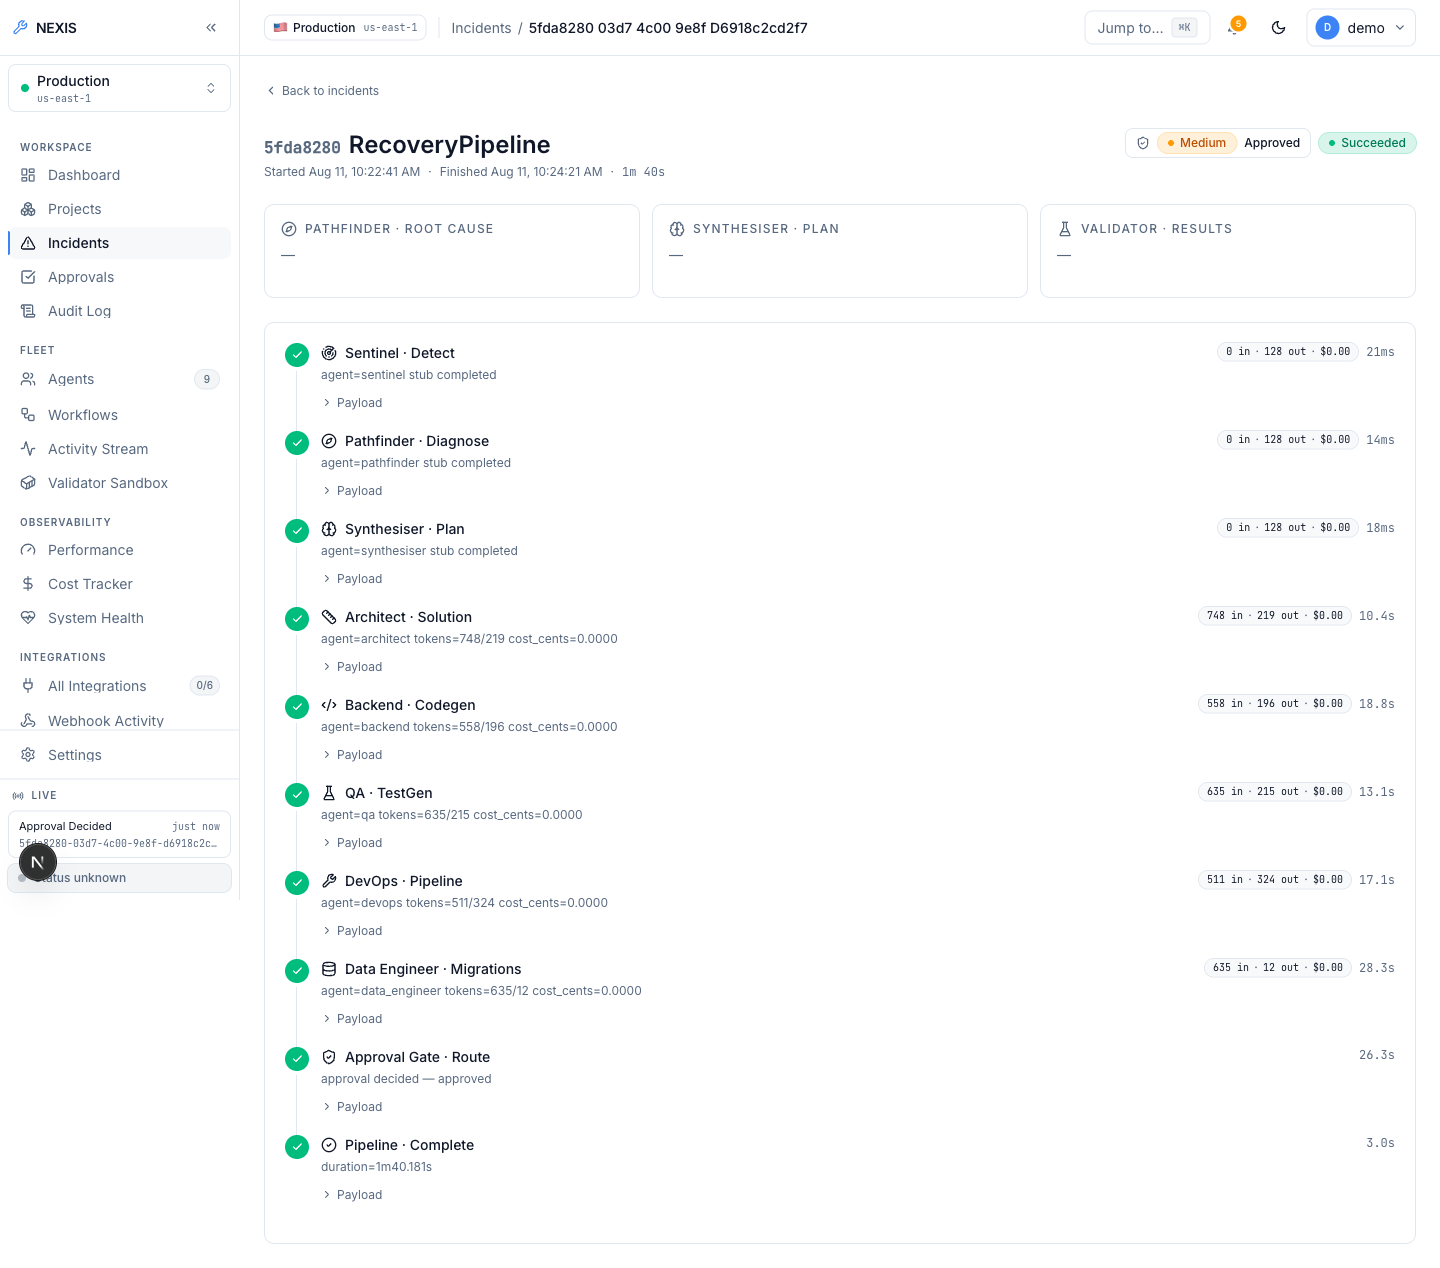
\includegraphics[width=0.85\textwidth]{../assets/screenshots/40-incident-full-success.png}
\caption{Fully Approved Run ( Medium severity, Approved, Succeeded; complete nine-step timeline in 1\,m\,40\,s with real per-agent token and cost figures ).}
\label{fig:fullsuccess}
\end{figure}

Finally, Figure~\ref{fig:payload} settles the question of whether the patch
itself is genuinely LLM-generated. It shows the expanded raw JSON payload of
the Backend agent's step: the actual unified diff produced by
\code{qwen2.5-coder:14b}, with \code{provider="ollama"} recorded in the
payload. The patch is model output parsed from a unified diff, not a
template retrieved from a fixture.

\begin{figure}[htbp]\centering
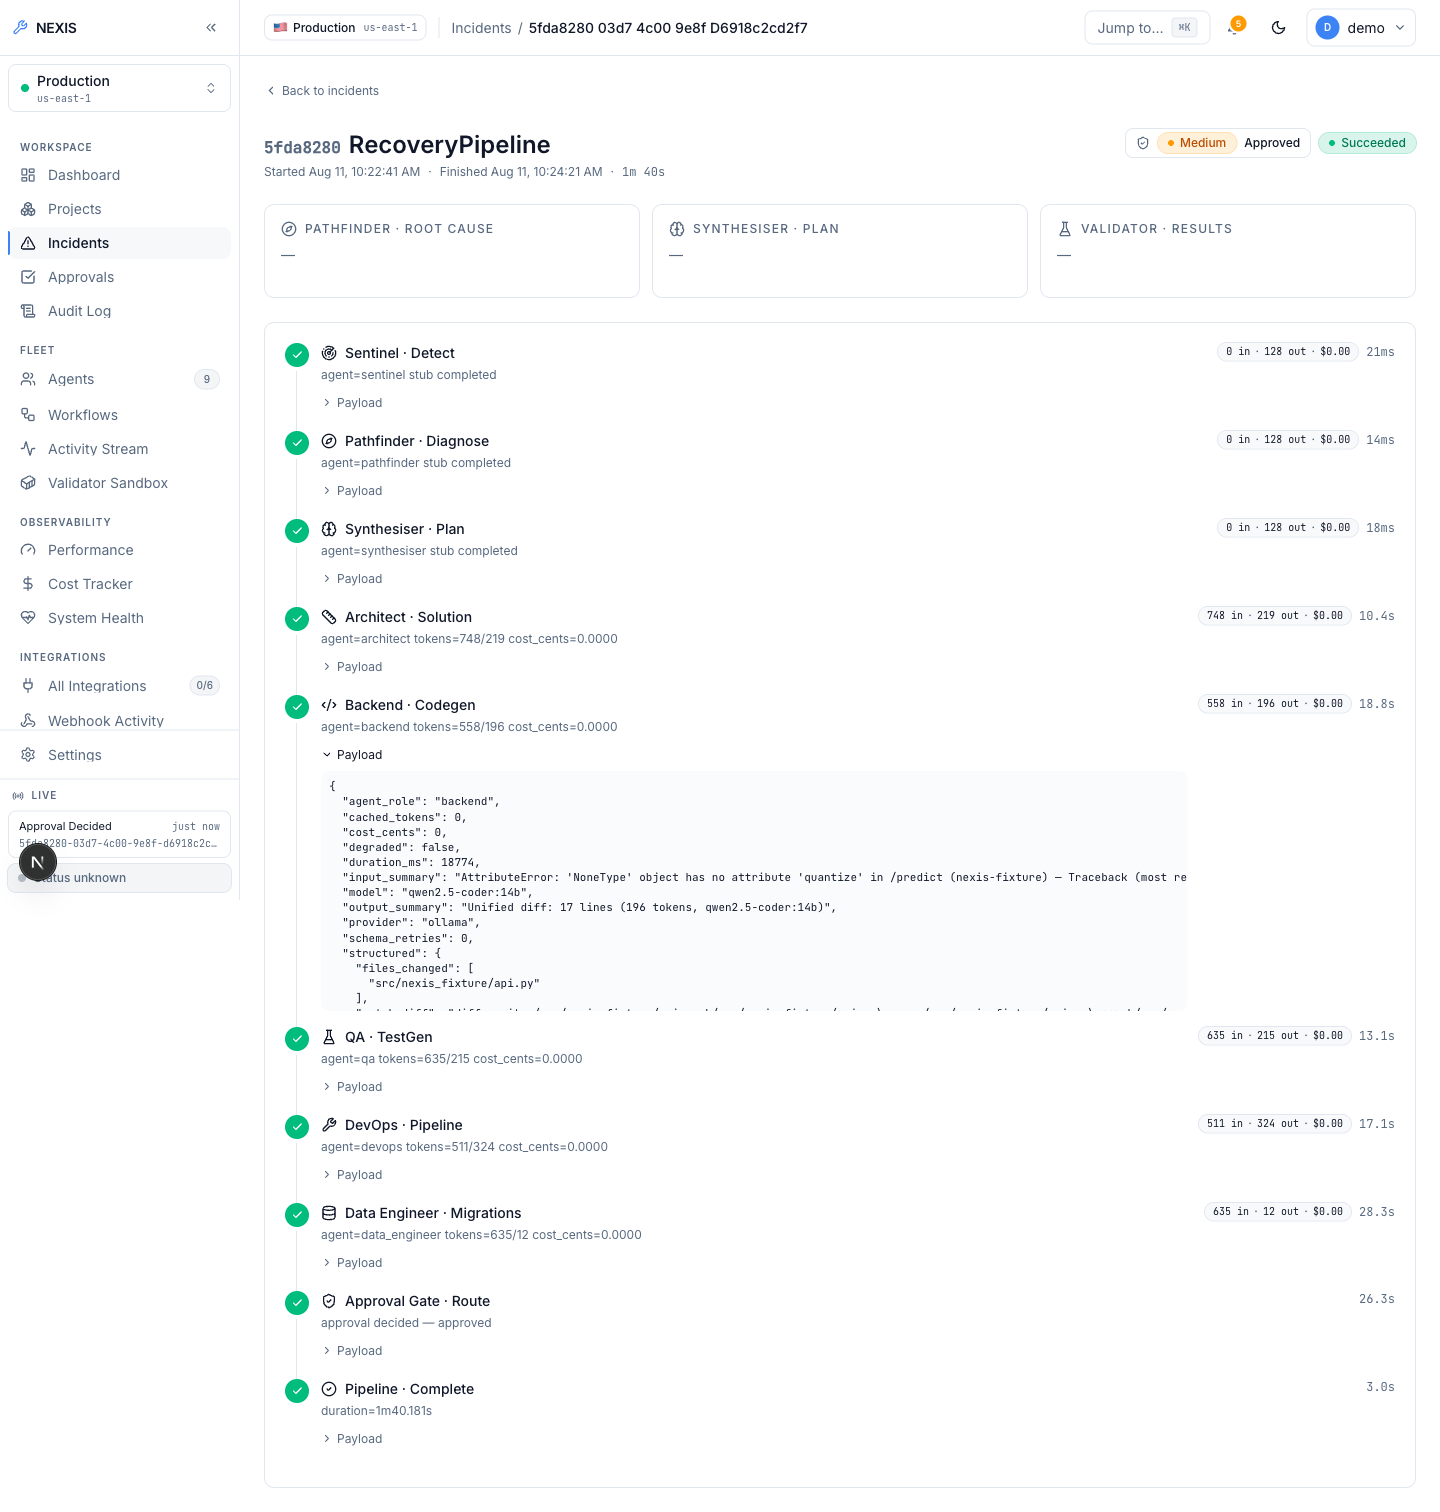
\includegraphics[width=0.85\textwidth]{../assets/screenshots/41-backend-payload-expanded.png}
\caption{Backend Payload, Expanded ( raw JSON evidence of the qwen2.5-coder:14b-generated unified diff, provider=``ollama'' ).}
\label{fig:payload}
\end{figure}

\subsection{Docker Preview-Deploy Engine (Ops Tab)}
\label{sec:opstab}

Each project detail page is organised into tabs. The Overview tab
(Figure~\ref{fig:projoverview}) summarises the project; Integrations
(Figure~\ref{fig:projintegrations}) manages the project's provider
connections, most importantly the GitHub repository binding; Recovery Policy
(Figure~\ref{fig:projpolicy}) configures per-project self-healing behaviour
such as rollback-on-SLO-breach; and Activity (Figure~\ref{fig:projactivity})
shows the project-scoped event history.

\begin{figure}[htbp]\centering
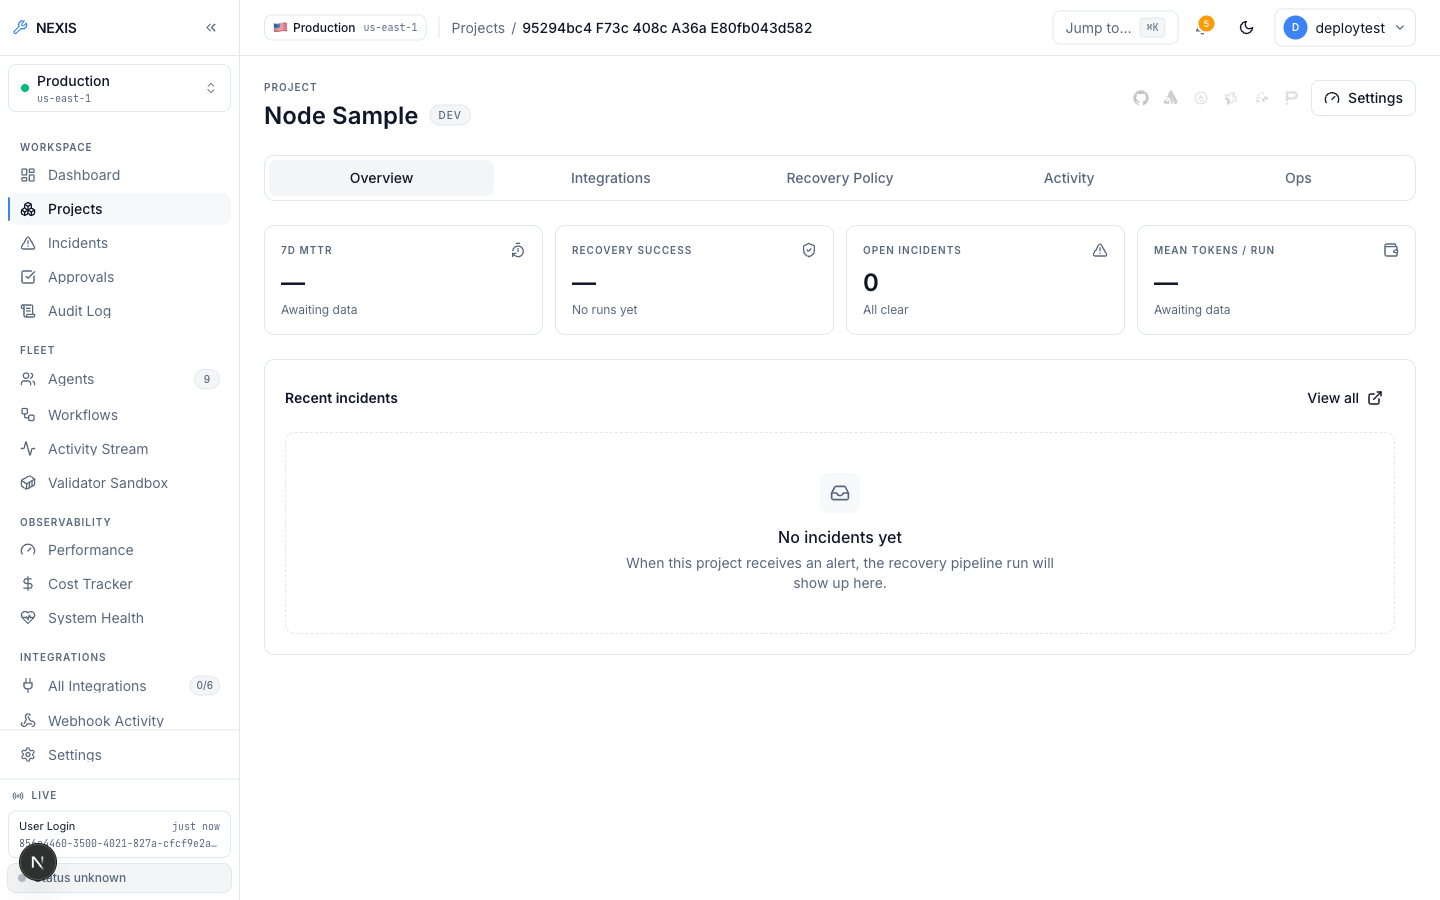
\includegraphics[width=0.85\textwidth]{../assets/screenshots/28-project-overview.png}
\caption{Project Overview Tab ( project summary and health ).}
\label{fig:projoverview}
\end{figure}

\begin{figure}[htbp]\centering
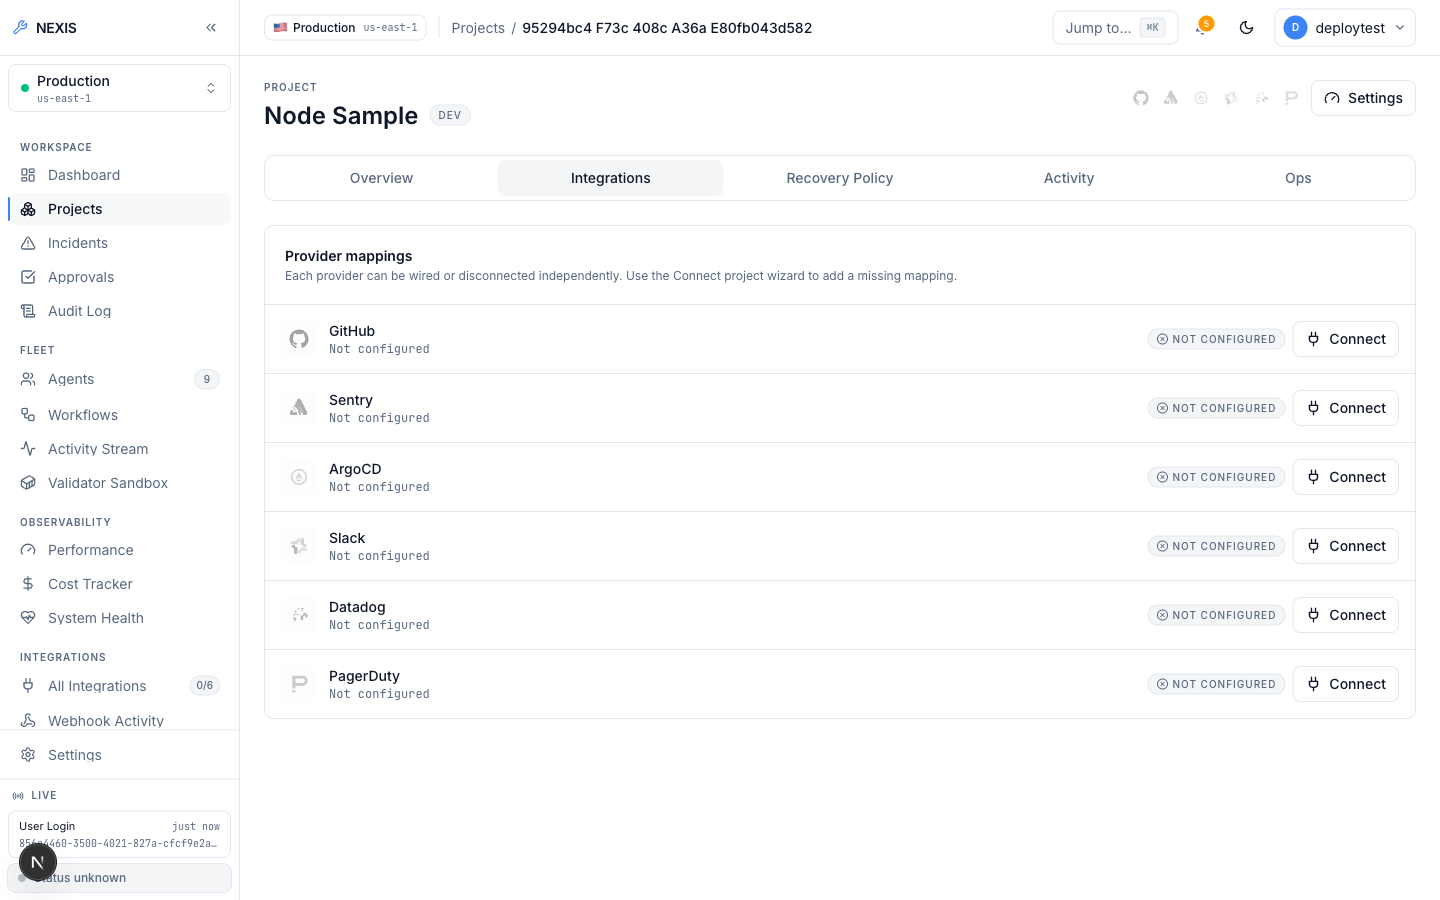
\includegraphics[width=0.85\textwidth]{../assets/screenshots/29-project-integrations.png}
\caption{Project Integrations Tab ( provider connections including the GitHub repository binding ).}
\label{fig:projintegrations}
\end{figure}

\begin{figure}[htbp]\centering
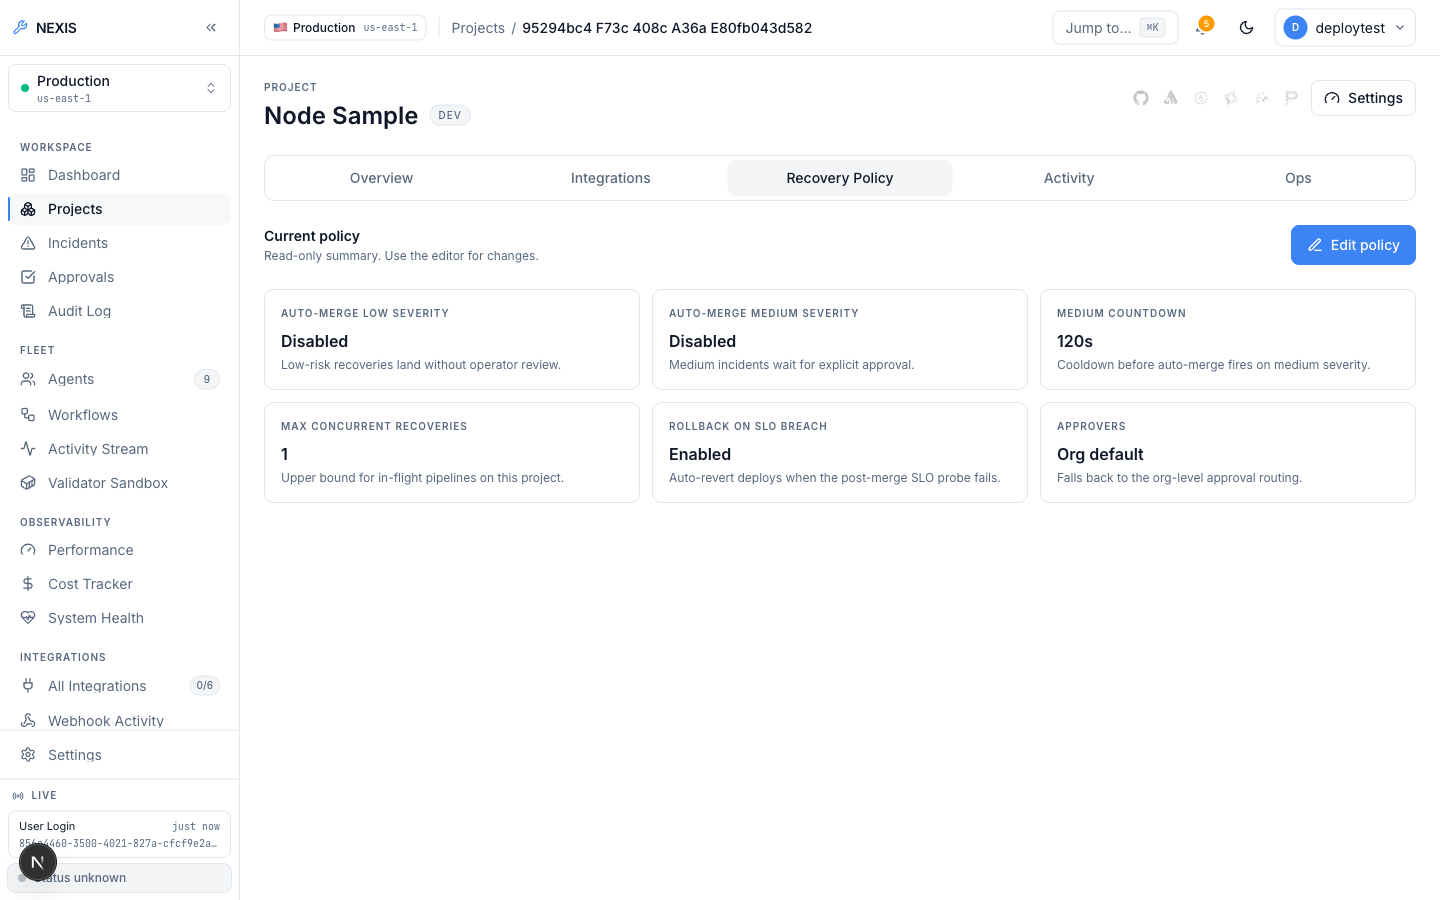
\includegraphics[width=0.85\textwidth]{../assets/screenshots/30-project-recovery-policy.png}
\caption{Project Recovery Policy Tab ( per-project self-healing configuration ).}
\label{fig:projpolicy}
\end{figure}

\begin{figure}[htbp]\centering
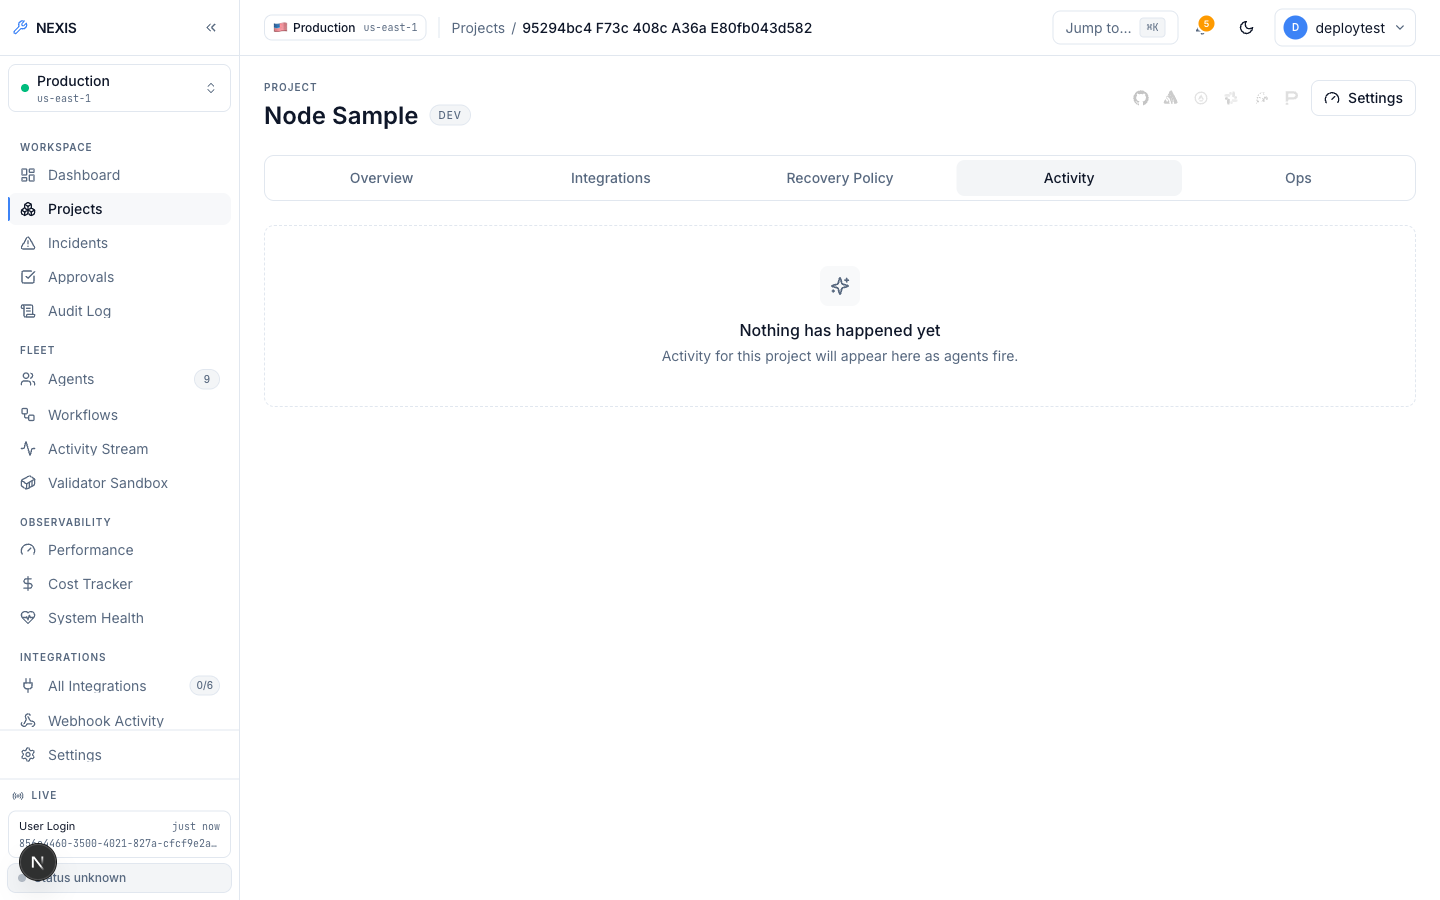
\includegraphics[width=0.85\textwidth]{../assets/screenshots/31-project-activity.png}
\caption{Project Activity Tab ( project-scoped event history ).}
\label{fig:projactivity}
\end{figure}

The Ops tab is the frontend to the preview-deploy engine.
Figure~\ref{fig:opsempty} shows its empty state before any deployment: the
Deploy action, live status area, and (once populated) the preview URL,
build/container logs, and deployment history.

\begin{figure}[htbp]\centering
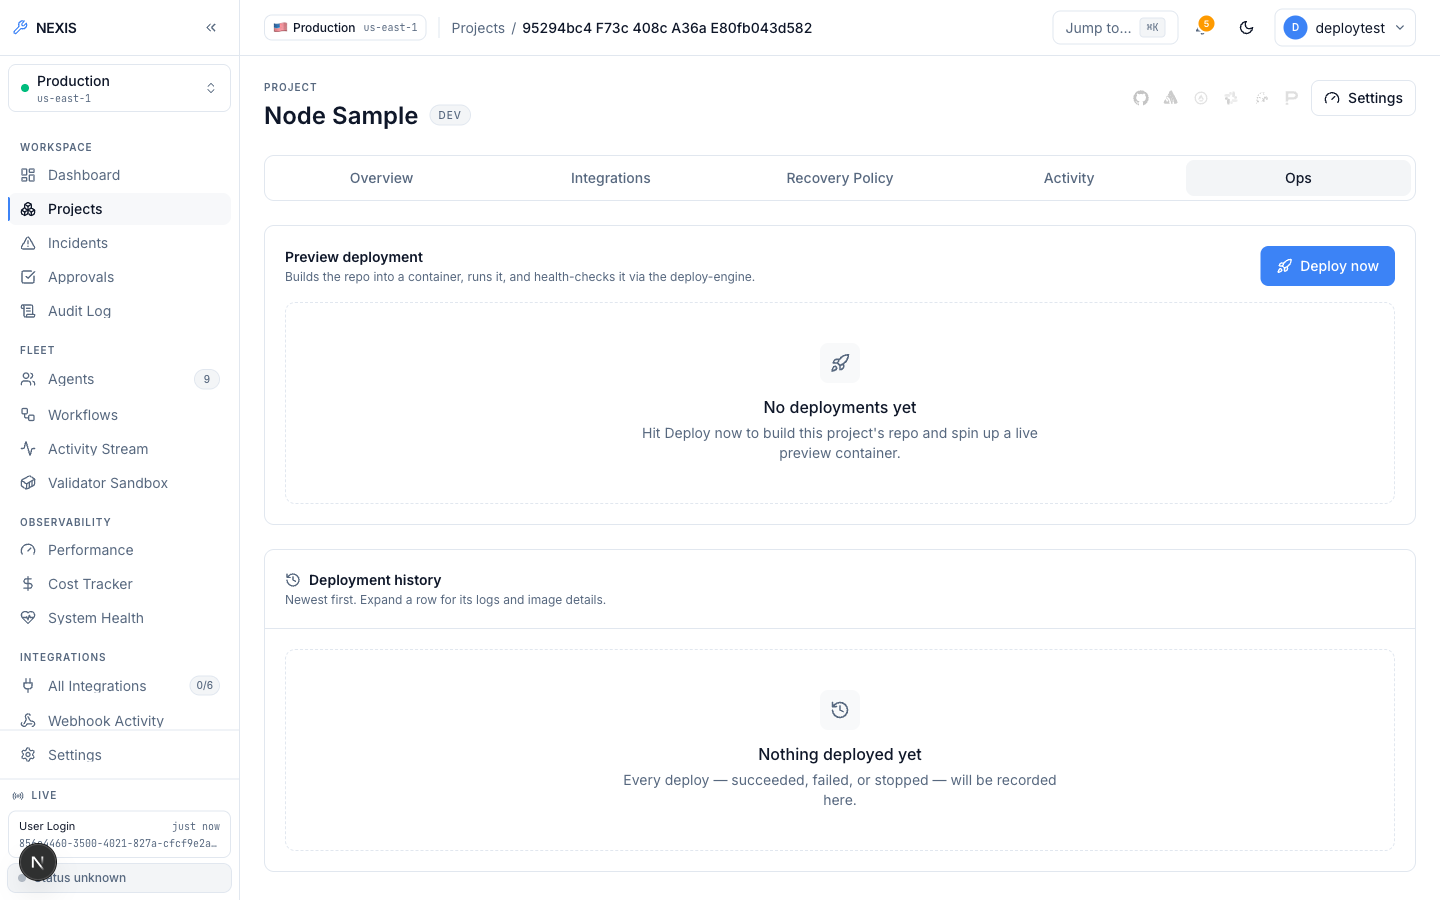
\includegraphics[width=0.85\textwidth]{../assets/screenshots/32-project-ops-empty.png}
\caption{Project Ops Tab, Empty State ( the Deploy panel before any deployment ).}
\label{fig:opsempty}
\end{figure}

Figure~\ref{fig:opsattempt} shows what happened when Deploy was clicked on a
project with no GitHub App connection in the evaluation environment: the
real API returned the validation error ``project has no github repository
bound'', which the UI surfaces verbatim. To be clear, this capture does
\emph{not} show a successful deploy --- it shows the real validation chain
rejecting a deploy request that cannot be fulfilled, which is the correct
behaviour. The limitation here is environmental (no GitHub App credentials
exist in the evaluation environment, as stated in Chapter~7's limitations),
not a defect in the engine.

\begin{figure}[htbp]\centering
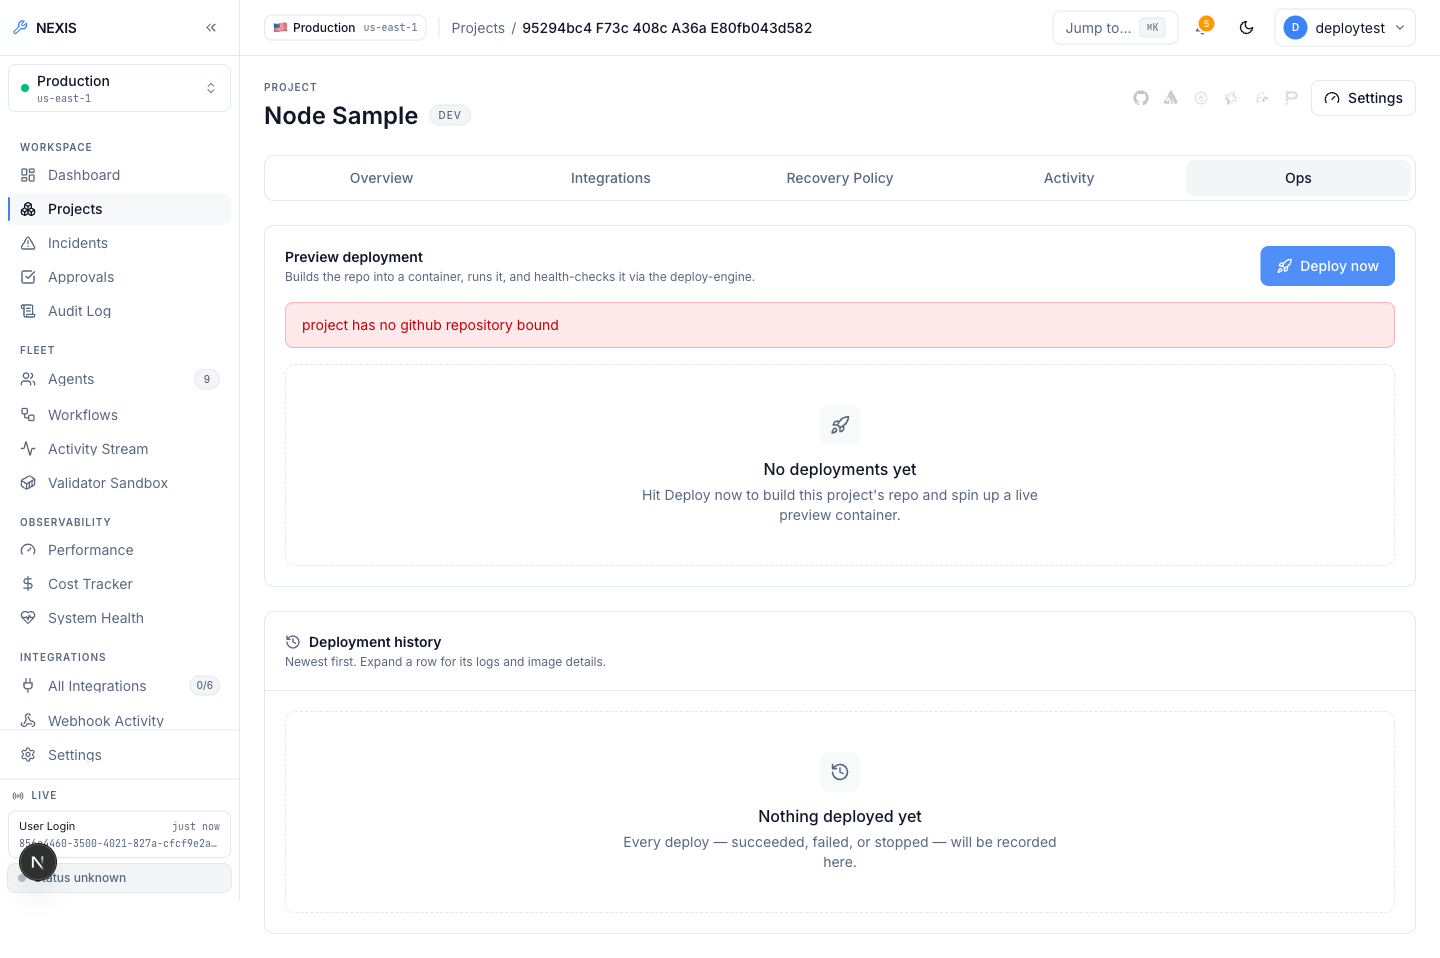
\includegraphics[width=0.85\textwidth]{../assets/screenshots/33-project-ops-deploy-attempt.png}
\caption{Project Ops Tab, Deploy Attempt ( a real validation error --- ``project has no github repository bound'' --- returned by the live API ).}
\label{fig:opsattempt}
\end{figure}

The engine itself, however, was proven live independently of that credential
limitation. Listing~\ref{lst:deployrun} reproduces verbatim the verified
end-to-end run recorded during this project: a real public repository
(\code{heroku/node-js-getting-started}, which contains no Dockerfile) was
cloned, its stack was detected as Node from marker files, a working
Dockerfile was generated, the image was built, the container was run under
resource limits, and an HTTP request to the returned preview URL served the
application's real rendered HTML page. The container was then stopped and
removed cleanly.

\begin{lstlisting}[caption={Verified live deploy-engine run},label={lst:deployrun}]
POST /v1/deploy  (repo: heroku/node-js-getting-started, no Dockerfile present)
-> 200 OK
  "status": "running", "dockerfile_source": "generated", "detected_stack": "node",
  "url": "http://localhost:54671", "image_tag": "nexis-preview-test-project:22d06076c357"
  build_log: "...npm ci... EXPOSE 3000... CMD [\"npm\",\"start\"]..."
  container_log: "Listening on 3000\nRendering 'pages/index' for route '/'"

GET http://localhost:54671/  -> real rendered HTML of the Node app (verified)

POST /v1/deploy/test-e2e-001/stop -> {"status":"stopped"}; container removed.
\end{lstlisting}

When a build or health check fails, the control plane inserts a real
incident with \code{source: "deploy\_engine"} into the same
Sentinel-to-RecoveryPipeline path used by every other incident source, so a
broken build or an unrecognised stack becomes a self-healing target like any
production fault.

\subsection{Projects, Agents, and Observability}

The Projects page (Figure~\ref{fig:projects}) lists the organisation's
projects as cards; new projects are created through the wizard in
Figure~\ref{fig:newproject}, which derives sensible defaults from the
project name. Each agent has its own detail page ---
Figure~\ref{fig:agentdetail} shows the Backend agent's --- and the Recovery
Pipeline page (Figure~\ref{fig:recoverypipeline}) presents the pipeline
structure itself.

\begin{figure}[htbp]\centering
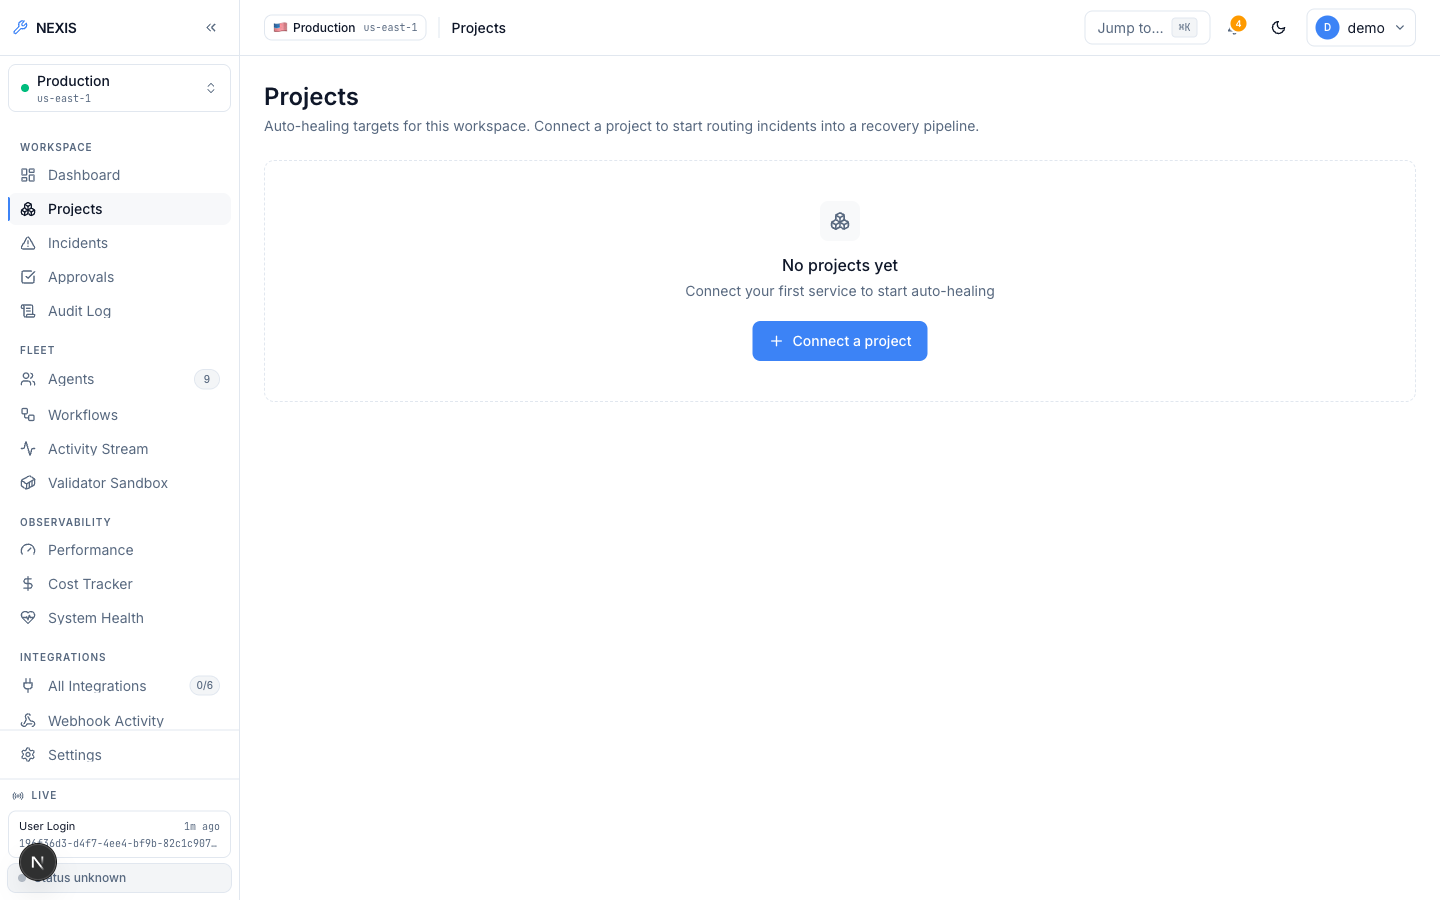
\includegraphics[width=0.85\textwidth]{../assets/screenshots/12-projects.png}
\caption{Projects Screen ( project cards with health indicators ).}
\label{fig:projects}
\end{figure}

\begin{figure}[htbp]\centering
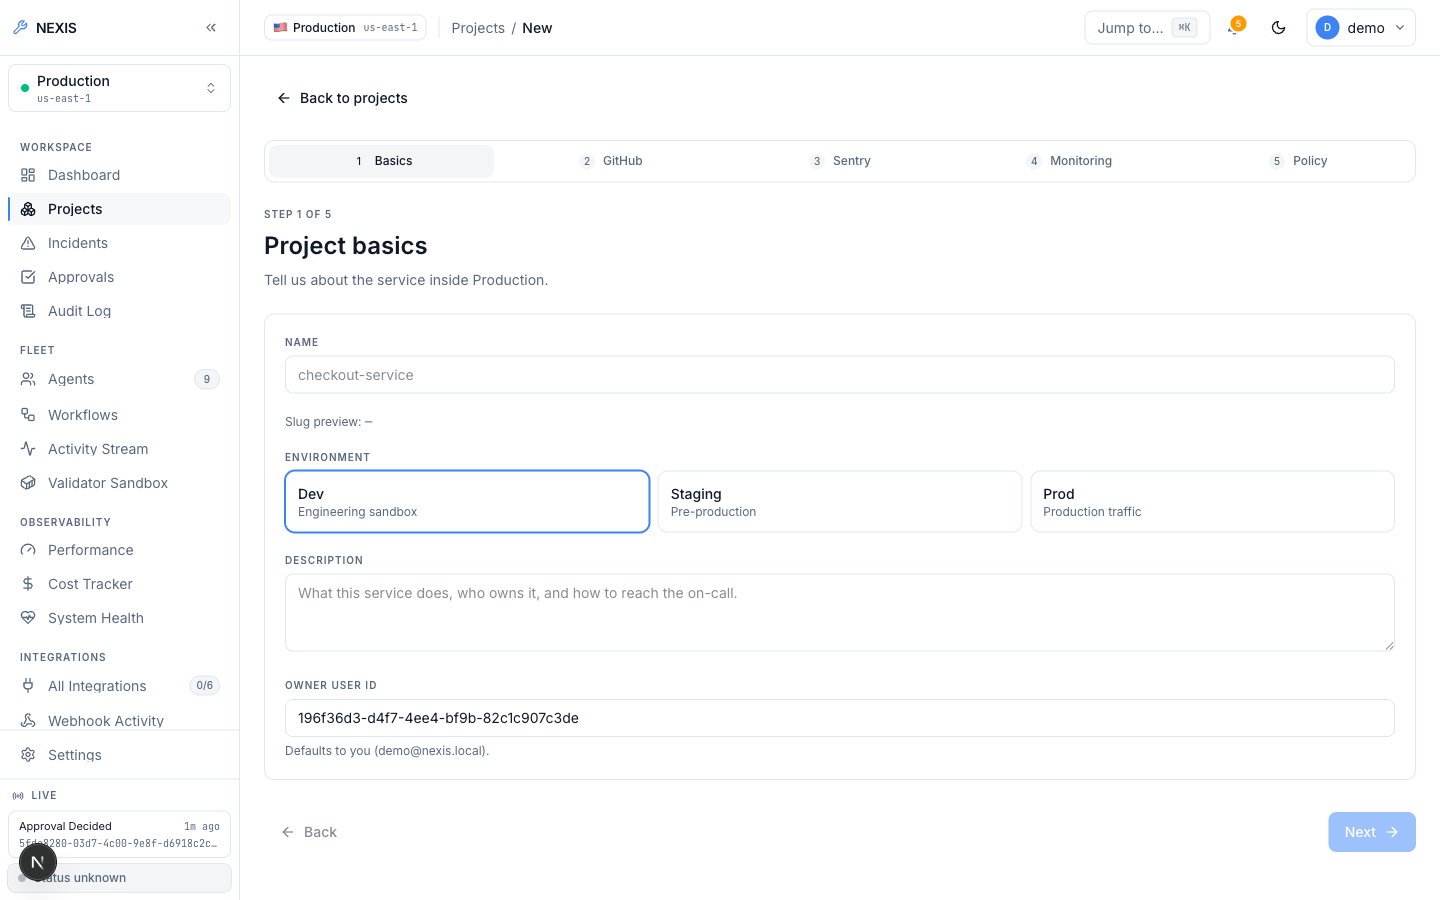
\includegraphics[width=0.85\textwidth]{../assets/screenshots/42-new-project-wizard.png}
\caption{New-Project Wizard ( guided project creation ).}
\label{fig:newproject}
\end{figure}

\begin{figure}[htbp]\centering
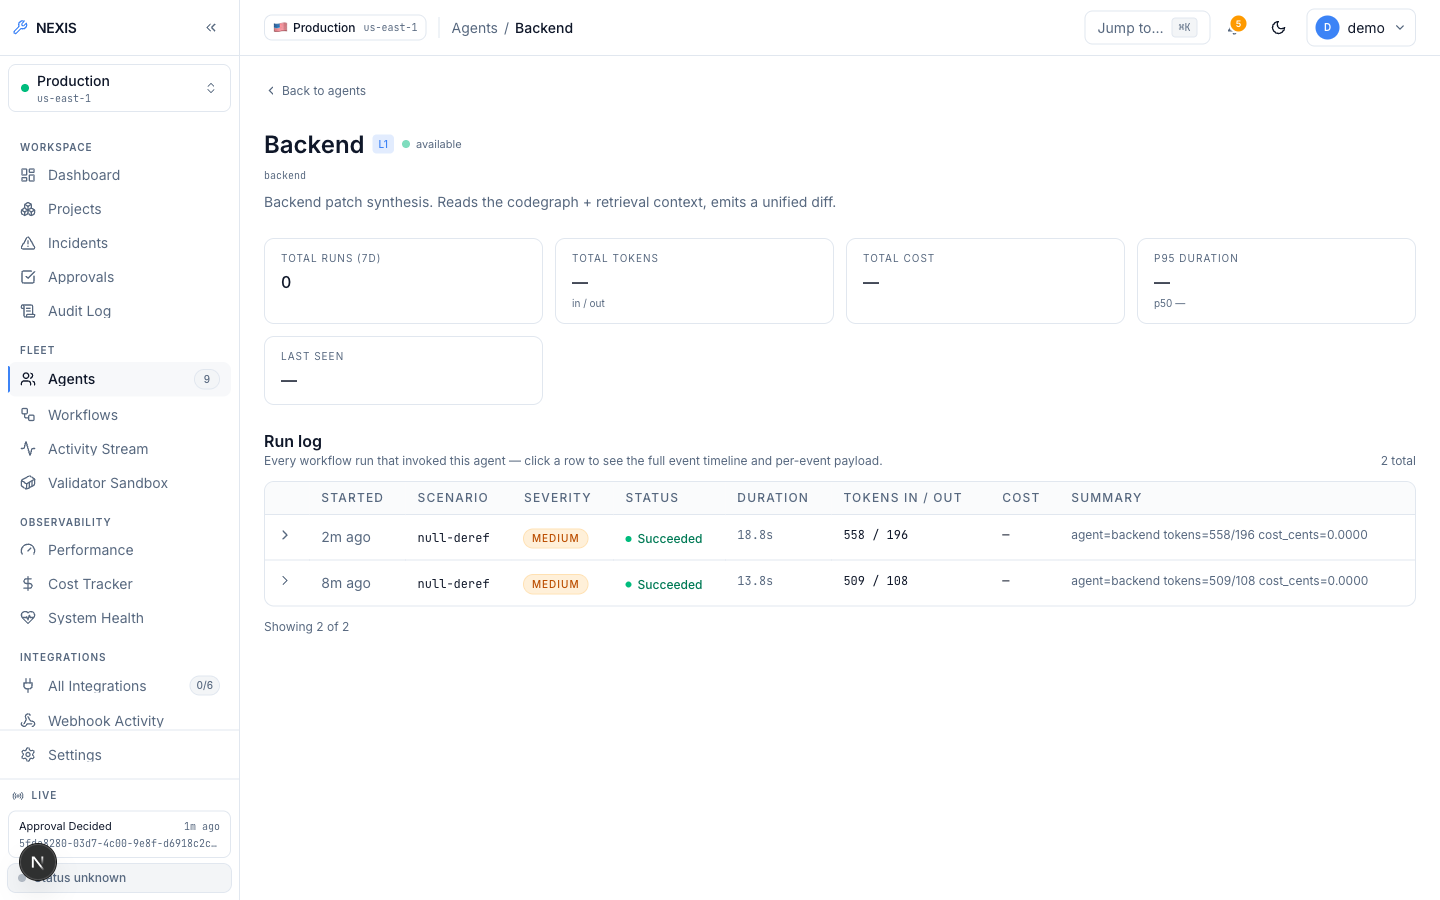
\includegraphics[width=0.85\textwidth]{../assets/screenshots/43-agent-detail-backend.png}
\caption{Agent Detail, Backend Agent ( per-agent configuration and run history ).}
\label{fig:agentdetail}
\end{figure}

\begin{figure}[htbp]\centering
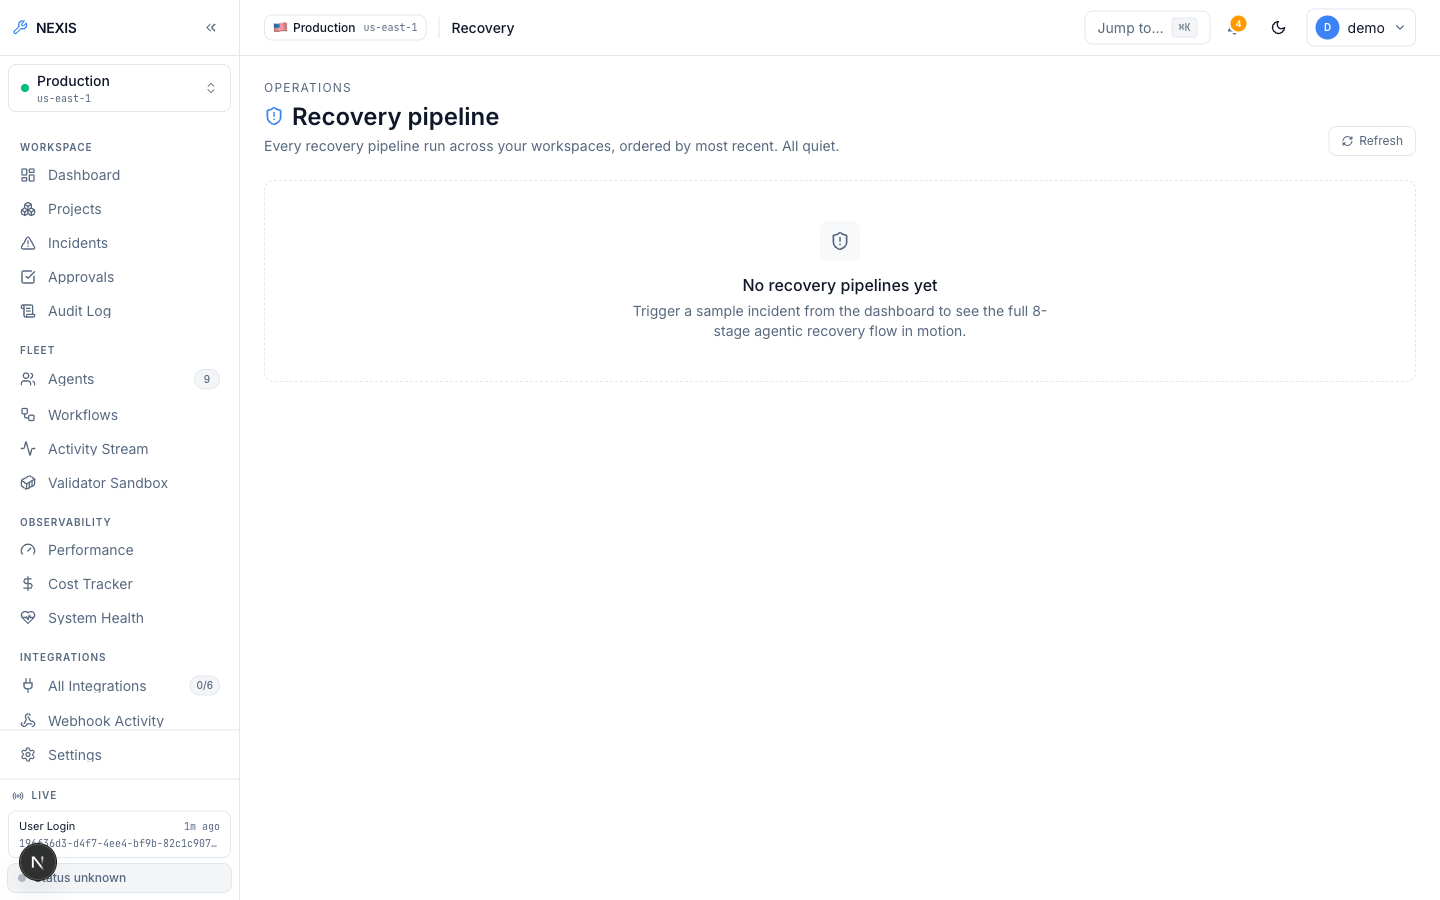
\includegraphics[width=0.85\textwidth]{../assets/screenshots/27-recovery-pipeline.png}
\caption{Recovery Pipeline Screen ( the nine-agent pipeline structure ).}
\label{fig:recoverypipeline}
\end{figure}

Observability is spread across four pages. Performance
(Figure~\ref{fig:performance}) charts pipeline latency and throughput; the
Cost Tracker (Figure~\ref{fig:cost}) rolls up the per-organisation token
ledger against a configurable daily budget; System Health
(Figure~\ref{fig:health}) fans out parallel dependency probes --- Postgres,
Redis, Neo4j, MinIO, Temporal --- under a bounded timeout and reports each
result; and the Eval Harness (Figure~\ref{fig:eval}) runs side-by-side
OpenAI-versus-Ollama provider comparisons across fixture incidents, with
persisted transcripts, cost accounting, and an admin-only CSV export. The
Knowledge Base page (Figure~\ref{fig:kb}) reports the status of the
pgvector-backed retrieval store.

\begin{figure}[htbp]\centering
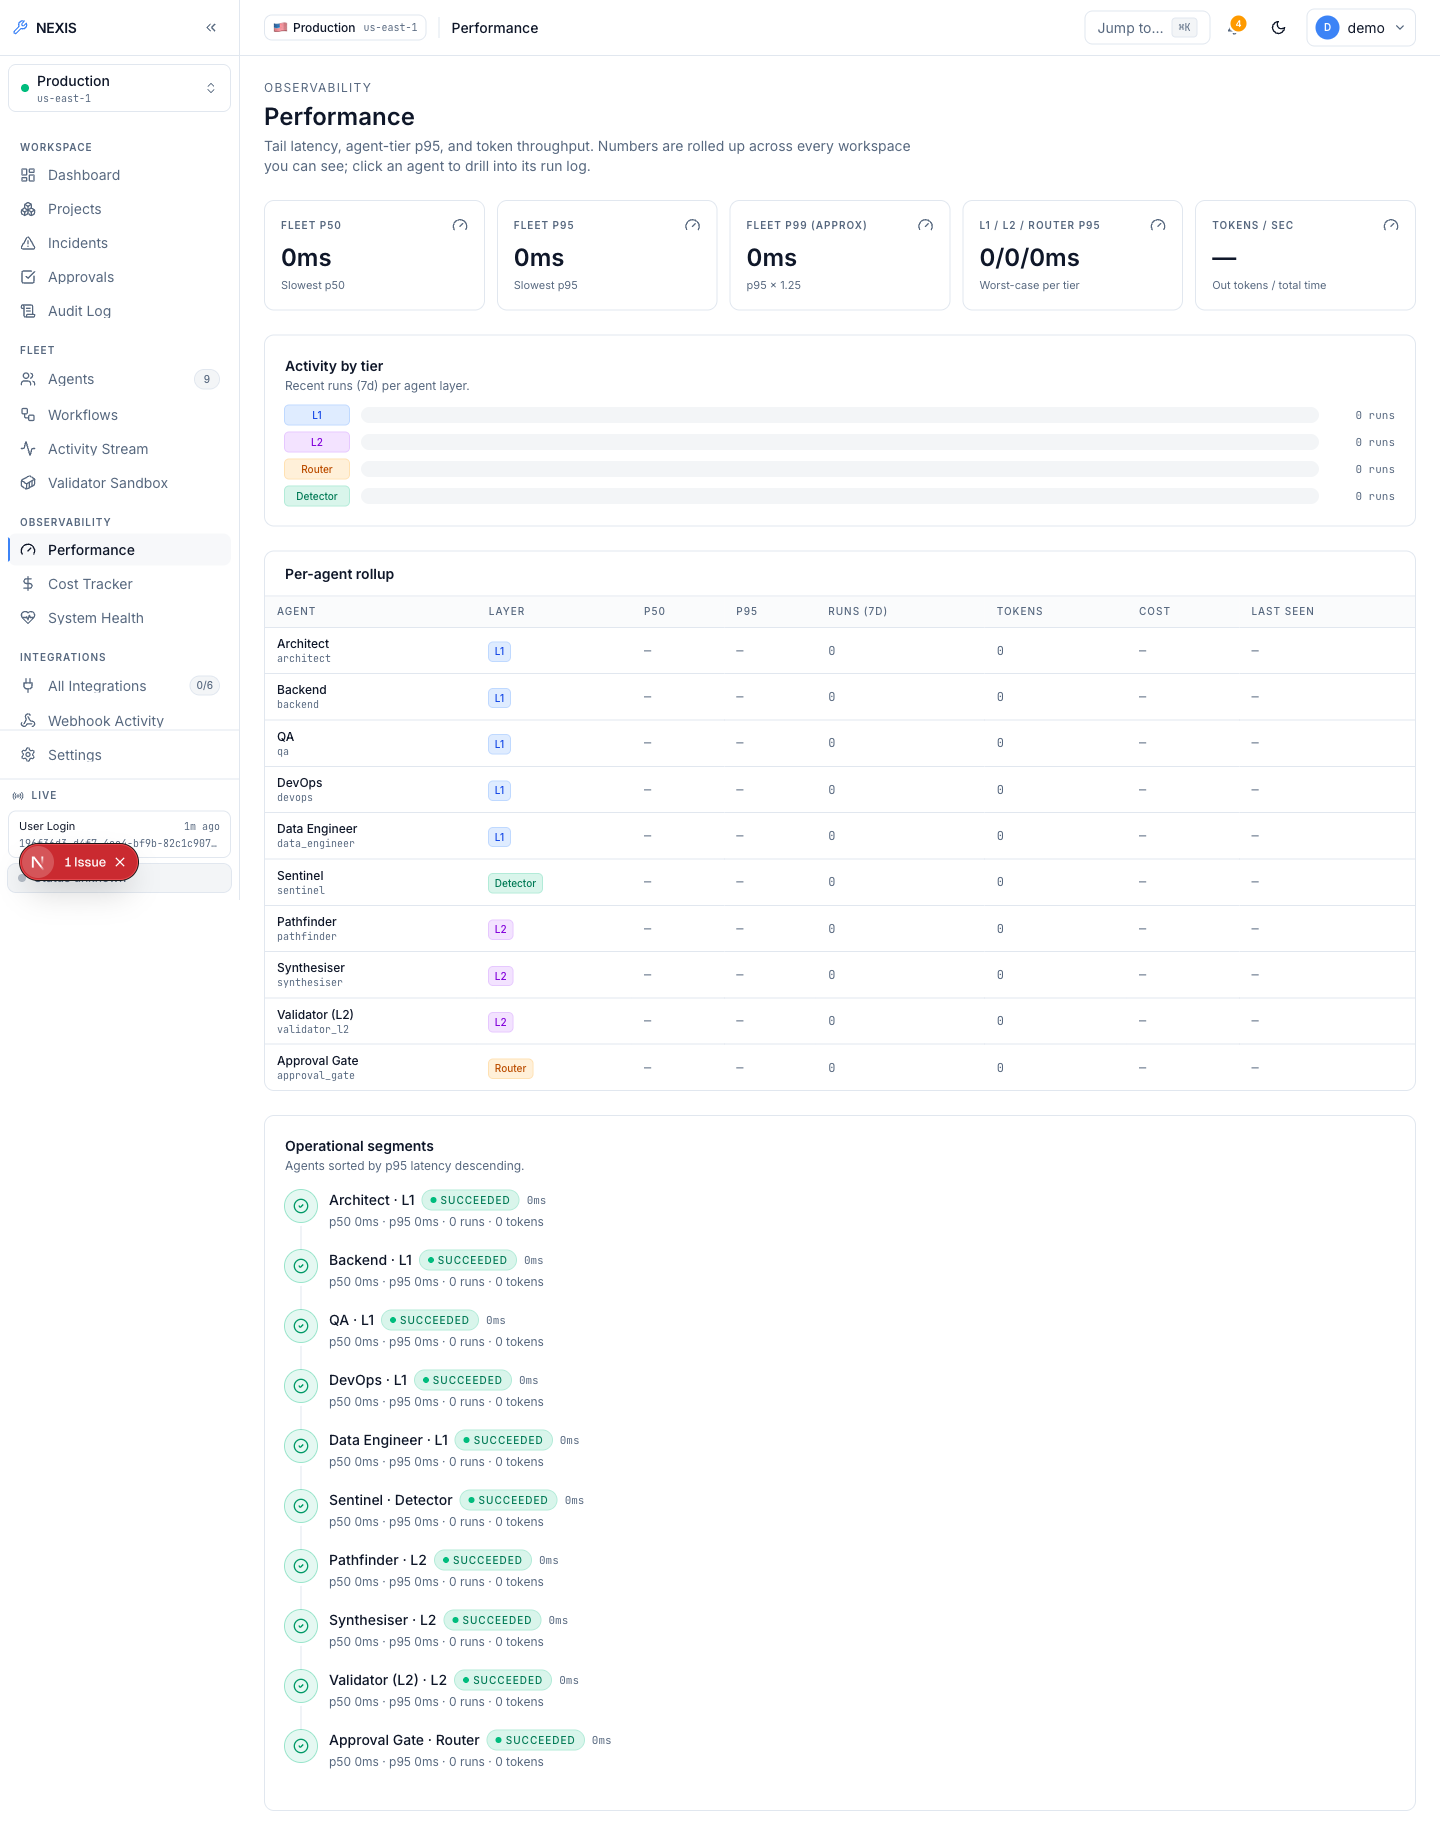
\includegraphics[width=0.85\textwidth]{../assets/screenshots/18-performance.png}
\caption{Performance Screen ( pipeline latency and throughput charts ).}
\label{fig:performance}
\end{figure}

\begin{figure}[htbp]\centering
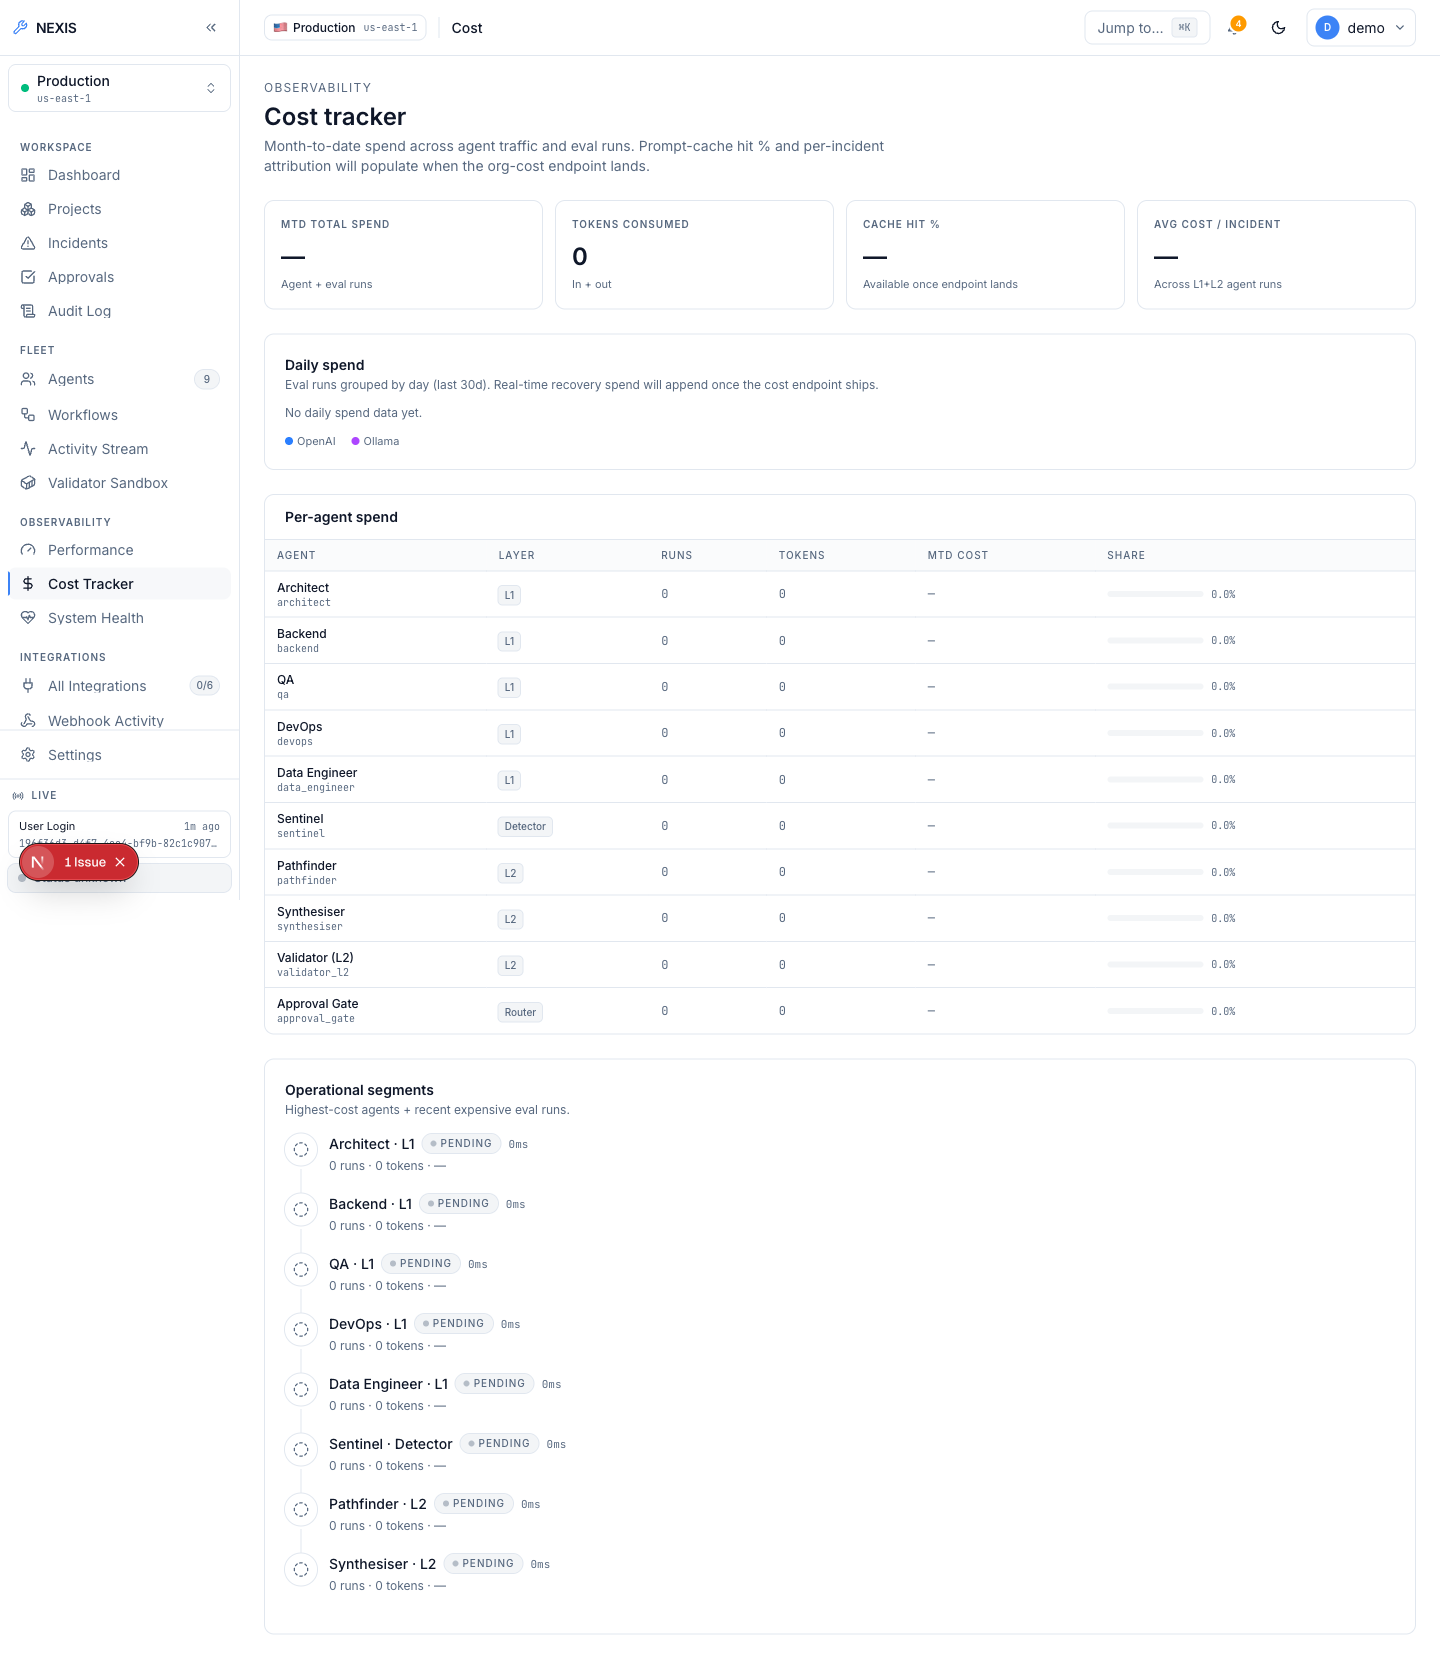
\includegraphics[width=0.85\textwidth]{../assets/screenshots/19-cost-tracker.png}
\caption{Cost Tracker ( per-organisation token ledger with daily budget ).}
\label{fig:cost}
\end{figure}

\begin{figure}[htbp]\centering
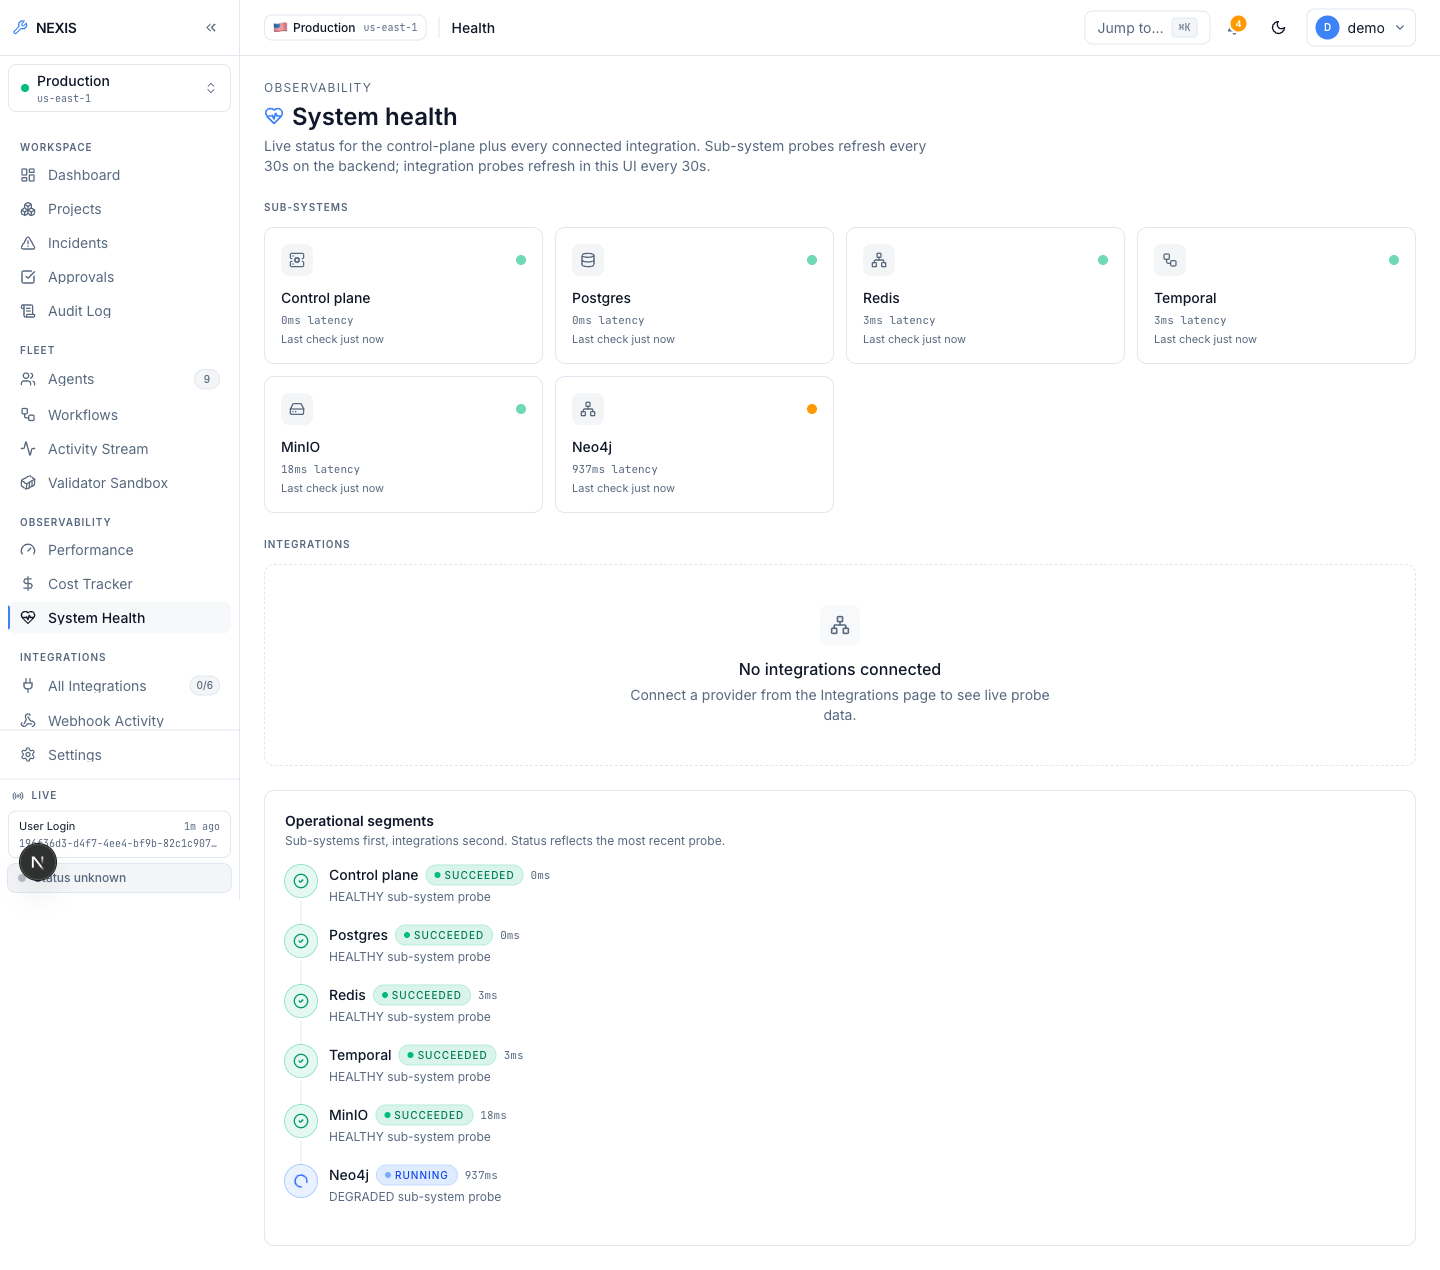
\includegraphics[width=0.85\textwidth]{../assets/screenshots/20-system-health.png}
\caption{System Health ( parallel dependency probes: Postgres, Redis, Neo4j, MinIO, Temporal ).}
\label{fig:health}
\end{figure}

\begin{figure}[htbp]\centering
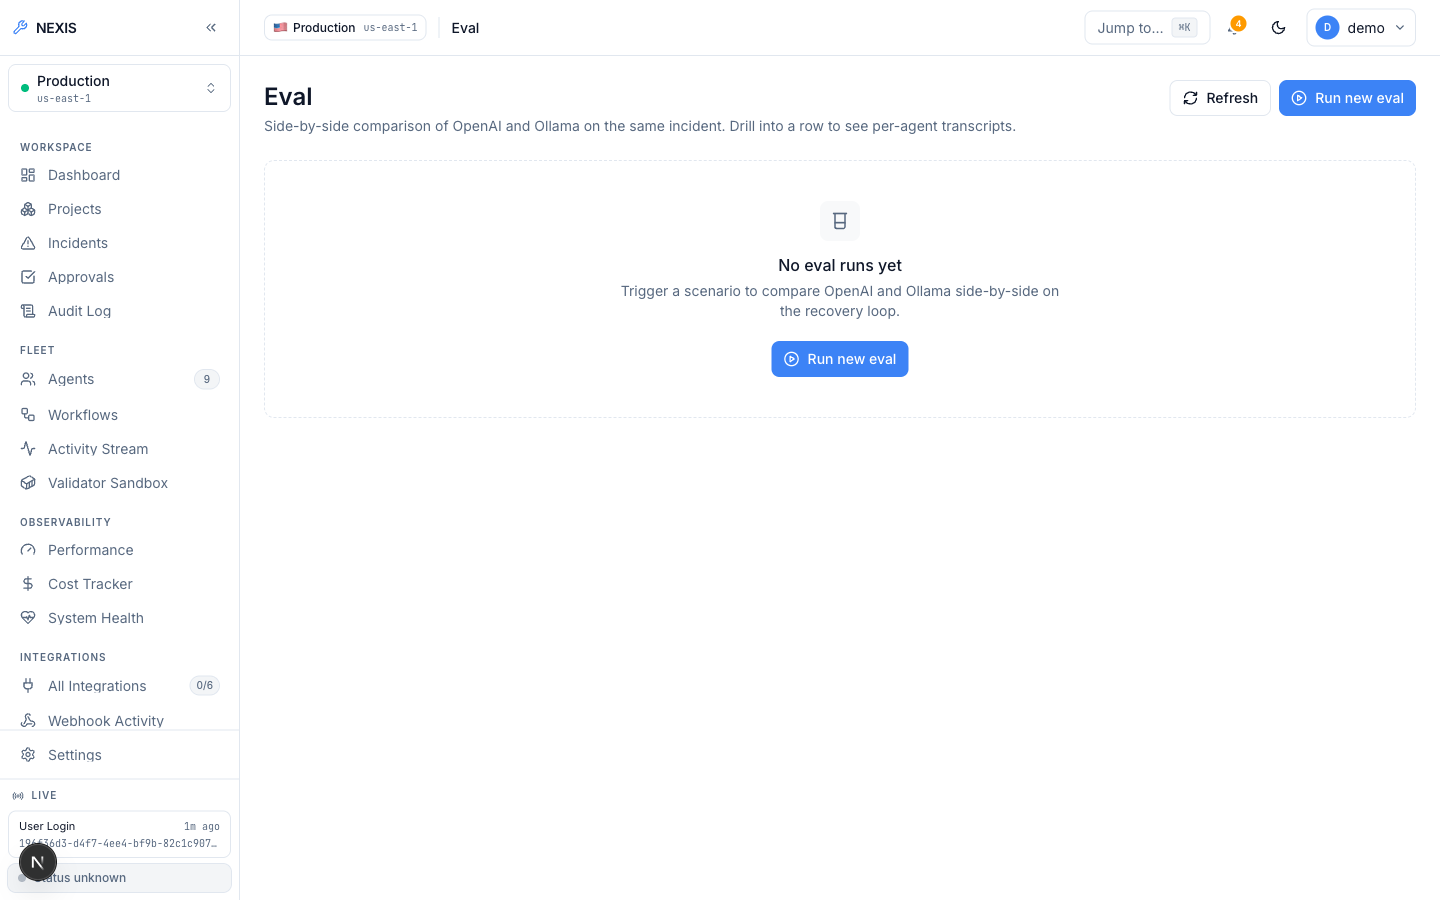
\includegraphics[width=0.85\textwidth]{../assets/screenshots/24-eval-harness.png}
\caption{Eval Harness ( side-by-side OpenAI-versus-Ollama comparison over fixture incidents ).}
\label{fig:eval}
\end{figure}

\begin{figure}[htbp]\centering
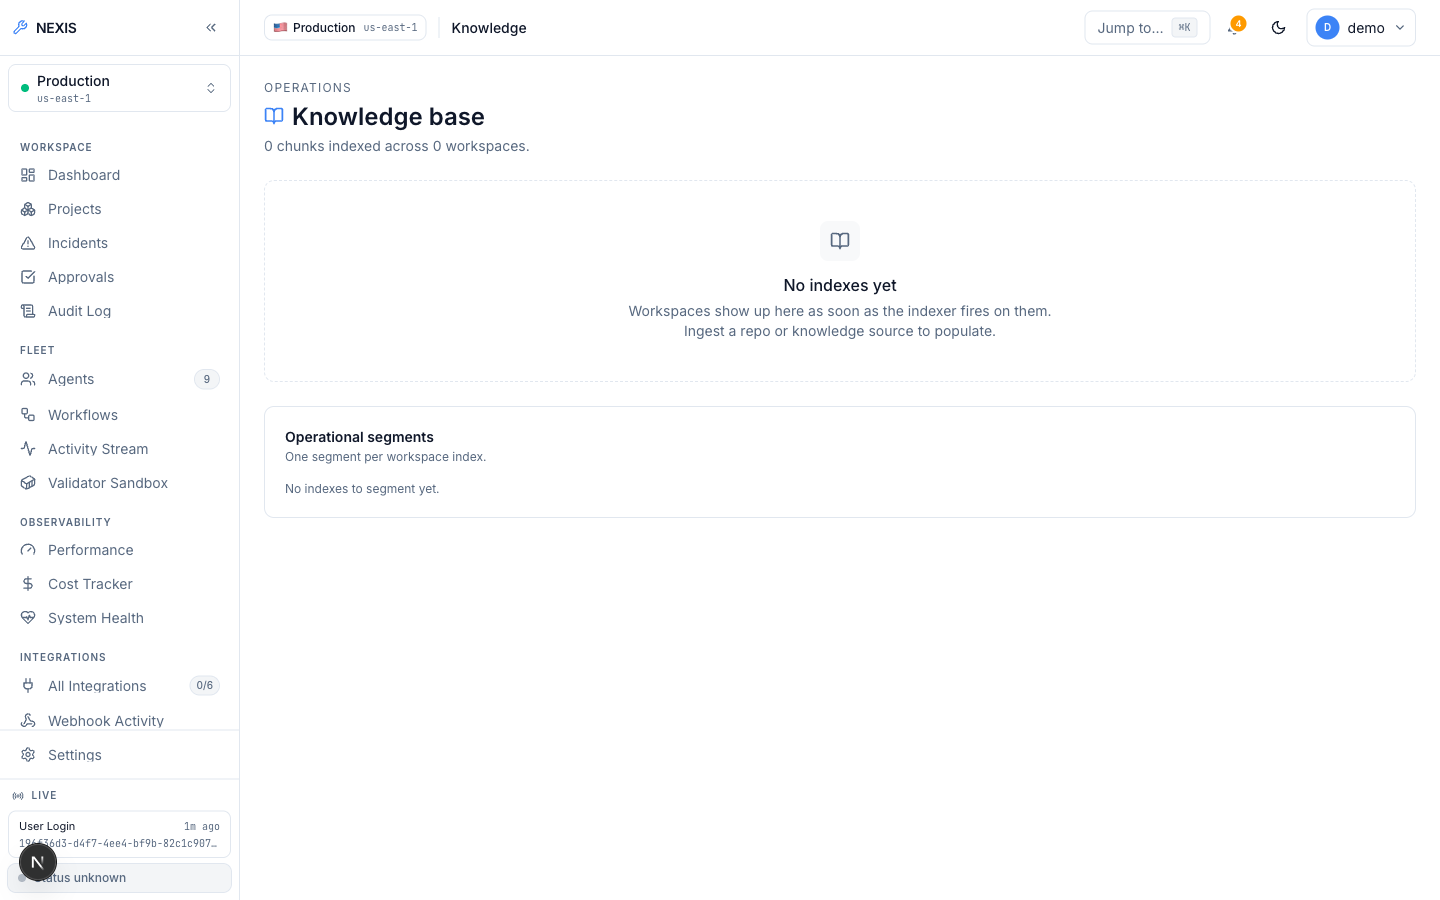
\includegraphics[width=0.85\textwidth]{../assets/screenshots/25-knowledge-base.png}
\caption{Knowledge Base ( pgvector-backed retrieval status ).}
\label{fig:kb}
\end{figure}

\subsection{Integrations}

The Integrations page (Figure~\ref{fig:integrations}) manages the external
providers the platform connects to: the GitHub App (installation, repository
listing, and webhook-driven incident creation on merged pull requests),
Sentry~\cite{sentry}, Datadog~\cite{datadog}, and PagerDuty~\cite{pagerduty}
as webhook-driven incident sources, Slack~\cite{slackapi} with OAuth install
and interactive one-click approve/reject directly from a Slack message,
Argo CD, and Stripe billing. Webhook Activity (Figure~\ref{fig:webhooks})
lists inbound webhook deliveries for debugging, and Connection Health
(Figure~\ref{fig:connhealth}) probes each configured integration and reports
its status.

\begin{figure}[htbp]\centering
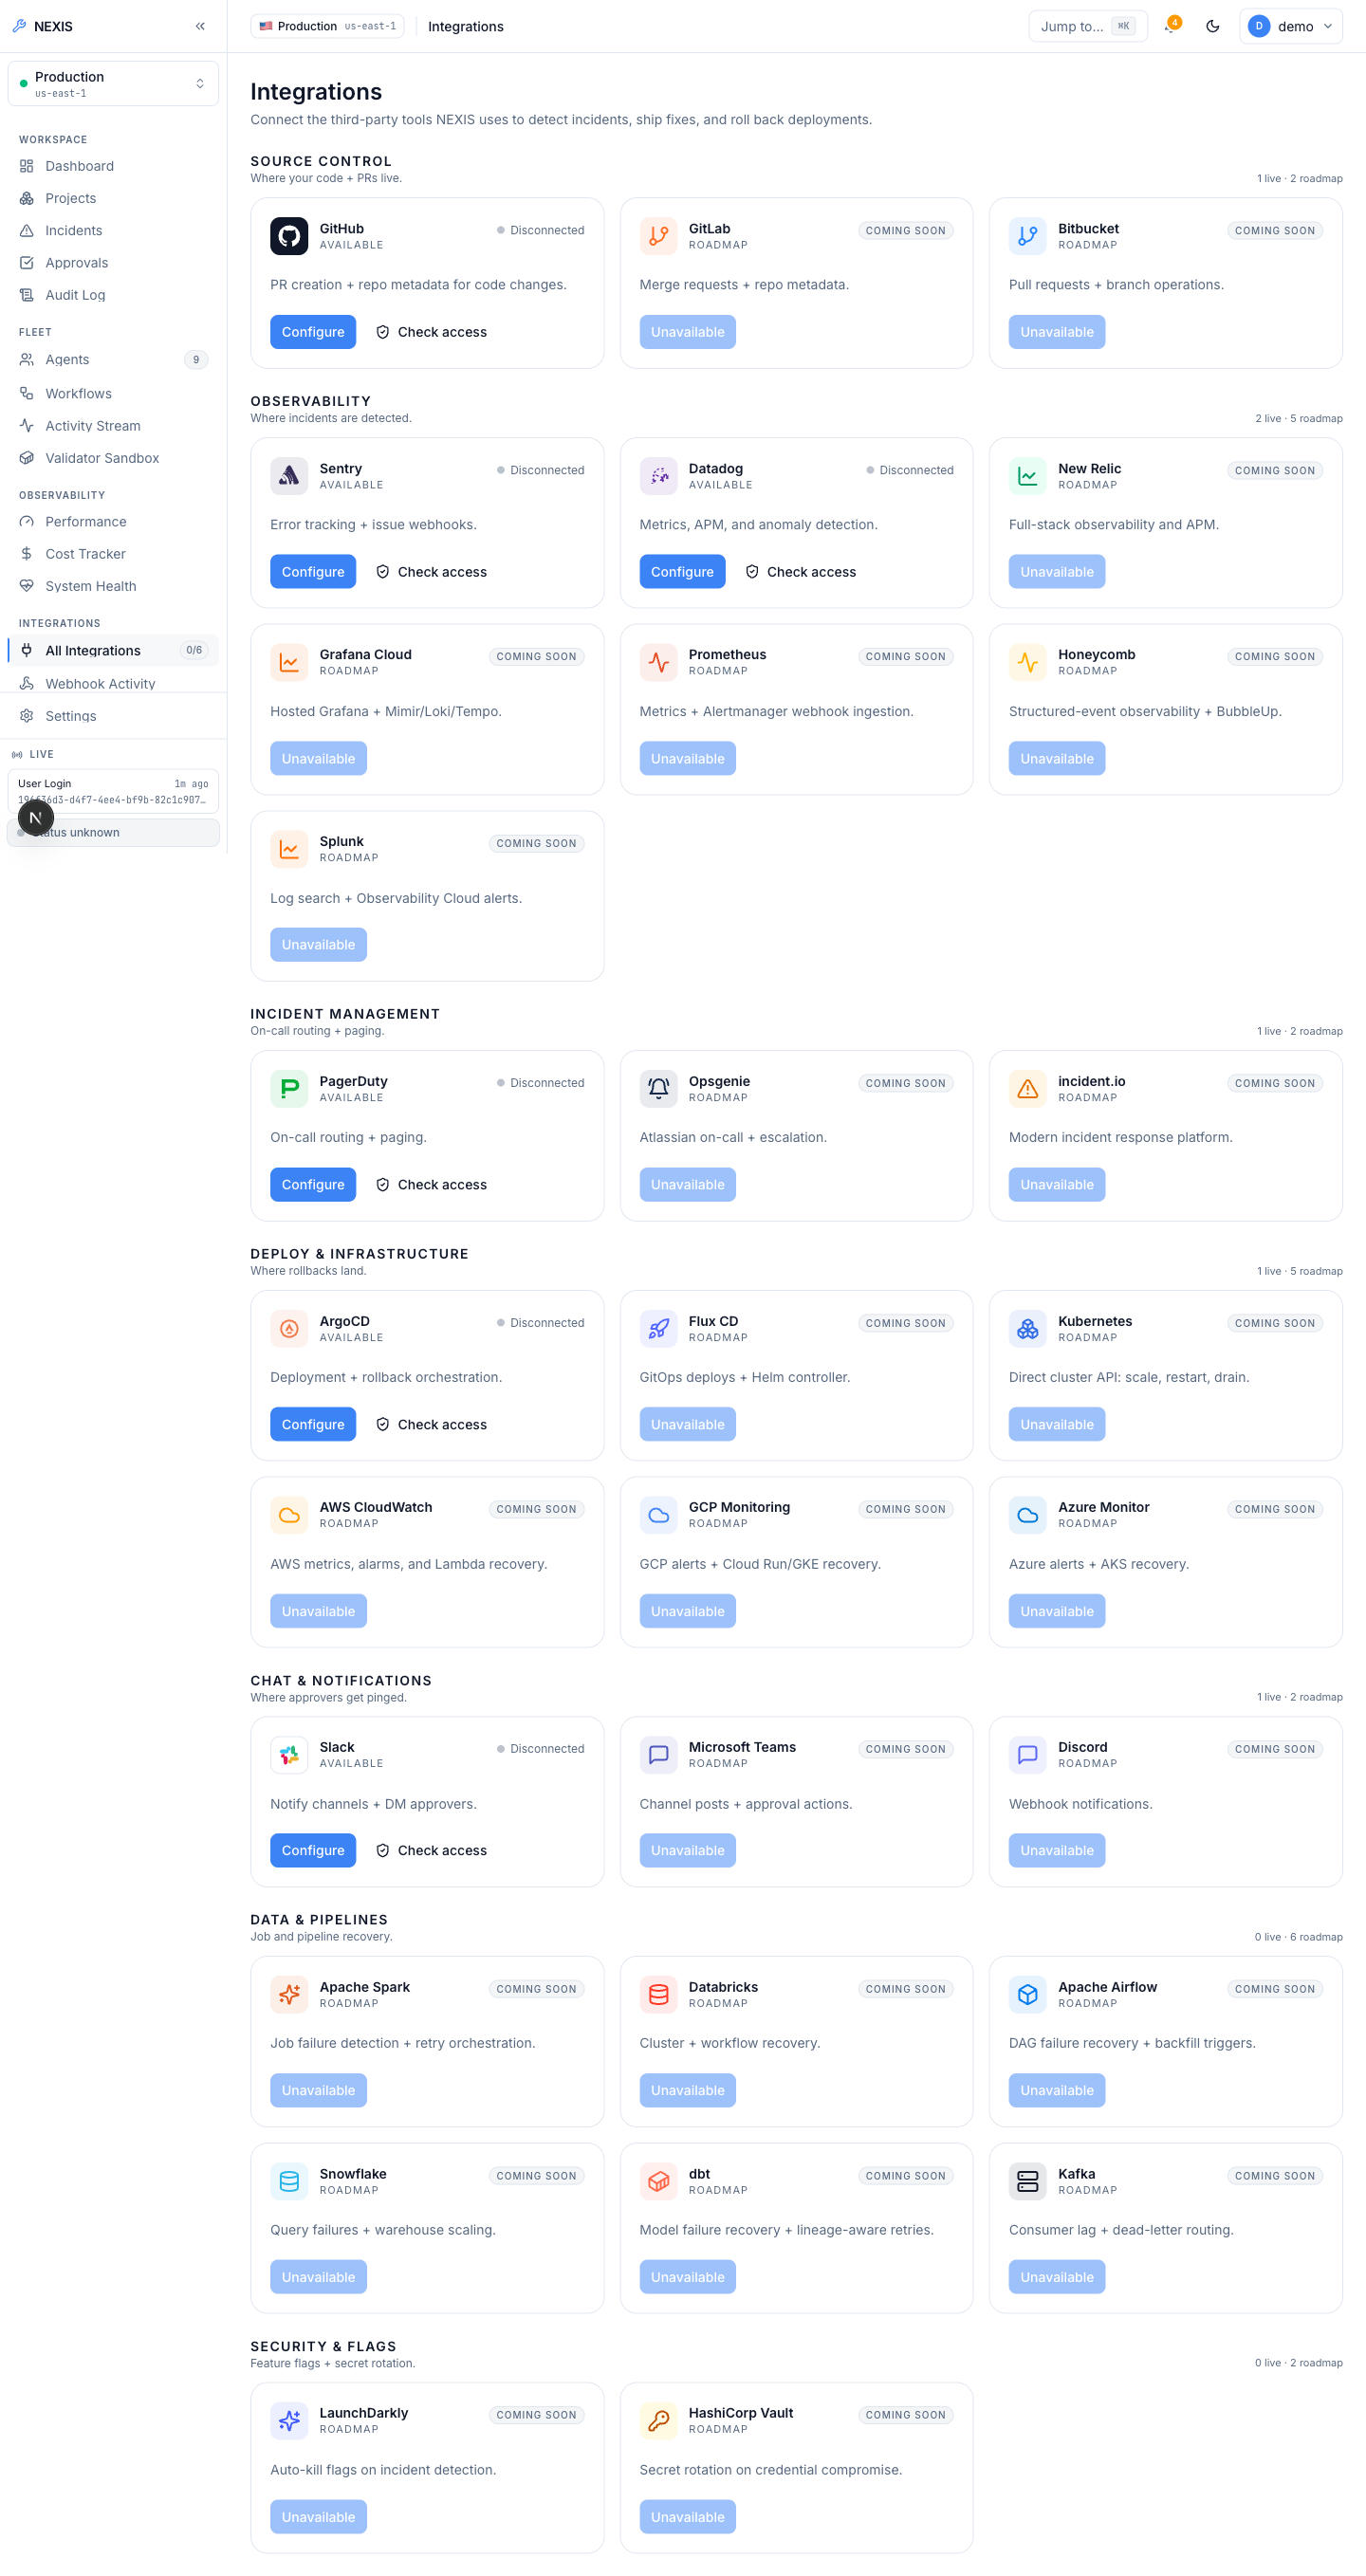
\includegraphics[width=0.85\textwidth]{../assets/screenshots/21-integrations.png}
\caption{Integrations Screen ( provider catalogue: GitHub App, Sentry, Datadog, PagerDuty, Slack, Argo CD, Stripe ).}
\label{fig:integrations}
\end{figure}

\begin{figure}[htbp]\centering
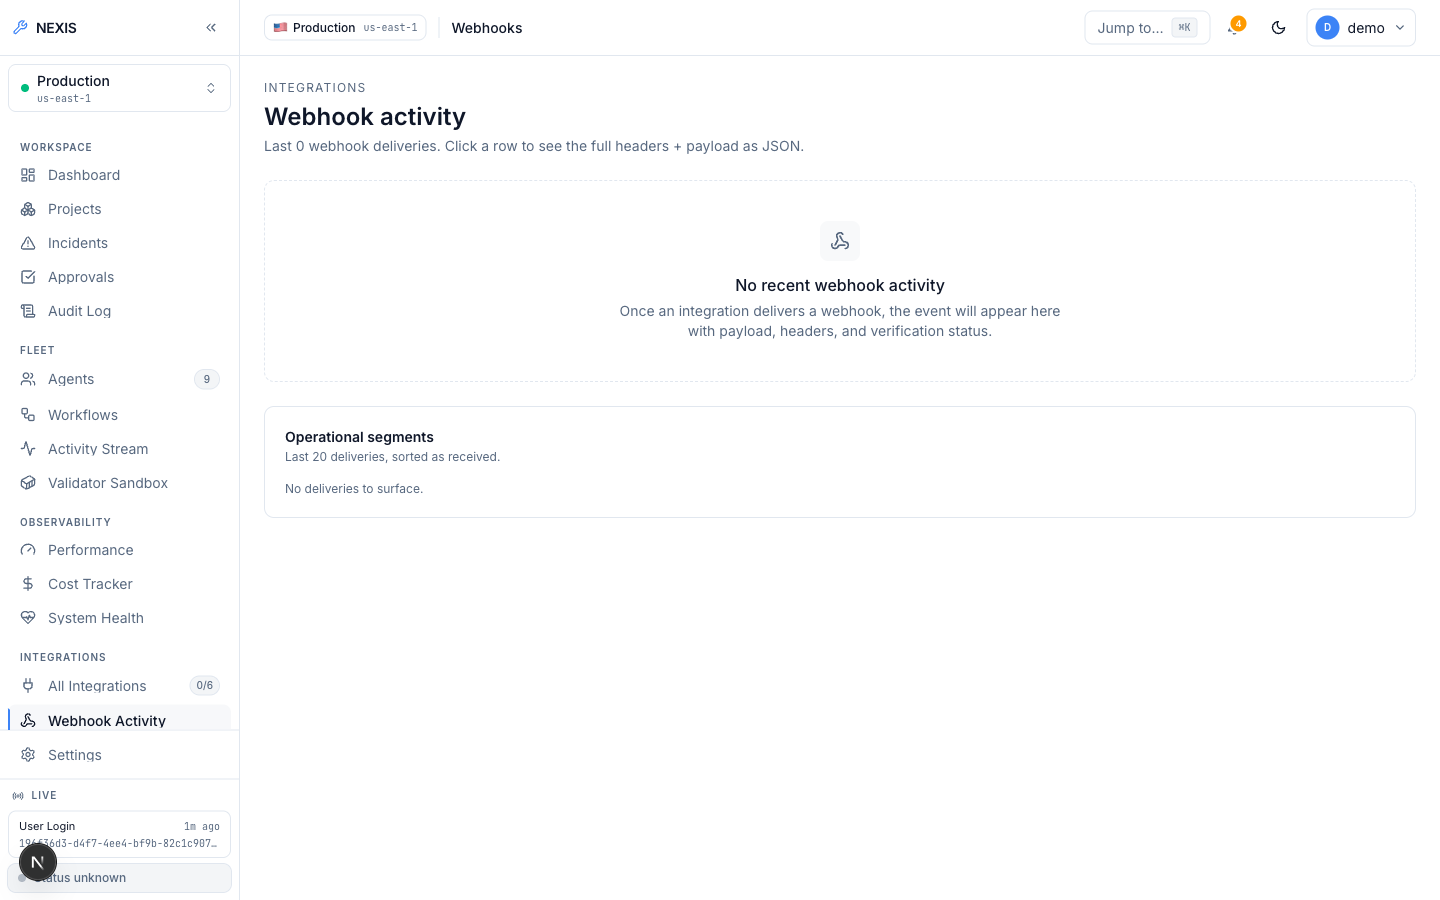
\includegraphics[width=0.85\textwidth]{../assets/screenshots/22-webhook-activity.png}
\caption{Webhook Activity ( inbound webhook delivery log ).}
\label{fig:webhooks}
\end{figure}

\begin{figure}[htbp]\centering
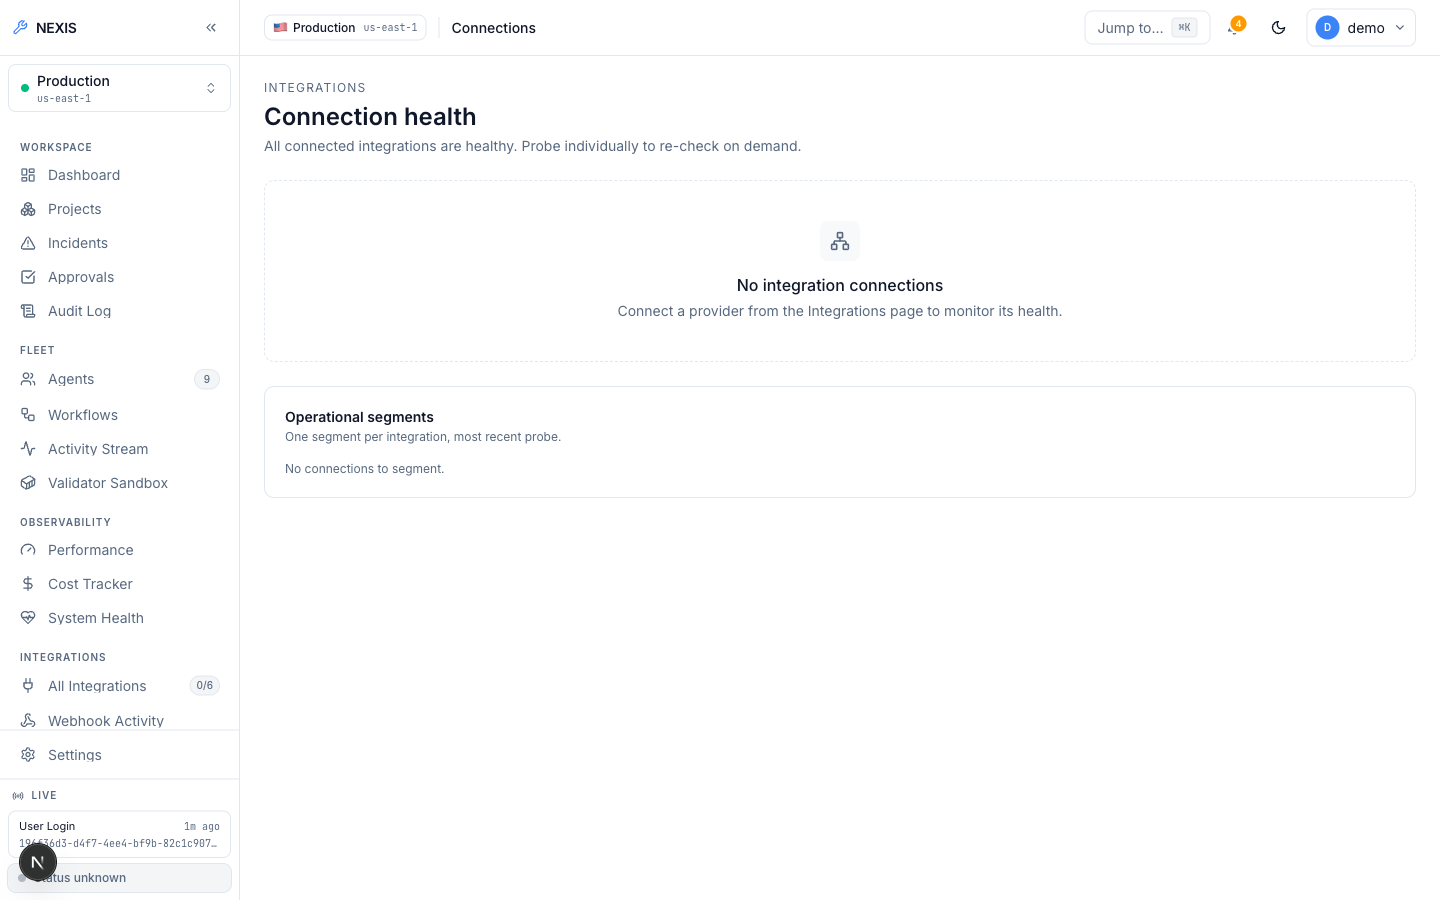
\includegraphics[width=0.85\textwidth]{../assets/screenshots/23-connection-health.png}
\caption{Connection Health ( per-integration health probes ).}
\label{fig:connhealth}
\end{figure}

\section{Database Schema}
\label{sec:schema}

Nexis stores its state in PostgreSQL~17. The schema has grown incrementally
across 33 sequential migrations, each tracked in version control alongside
the code that depends on it. Multi-tenancy is enforced in the database
itself rather than in application code: nearly every table carries an
organisation identifier, and PostgreSQL Row-Level Security
policies~\cite{pgrls} restrict every query to the calling organisation's
rows. A request-scoped transaction binds \code{app.current\_org\_id} for
each API request, so even a query that omits an explicit \code{WHERE}
clause on the organisation cannot read or write another tenant's data.

Table~\ref{tab:schema} summarises the key tables. Two deliberate exceptions
to org-scoping exist: \code{users} is a global identity table (a person may
belong to several organisations, with tenancy applied through
\code{org\_members}), and \code{sessions} is scoped to the owning user
rather than to an organisation, since a login session belongs to a person,
not a tenant.

\begin{table}[htbp]
\caption{Key tenant-scoped tables in the Nexis PostgreSQL schema.}
\label{tab:schema}
\centering
\small
\begin{tabular}{@{}p{3.6cm}p{7.2cm}p{2.9cm}@{}}
\toprule
\textbf{Table} & \textbf{Purpose} & \textbf{RLS scope} \\
\midrule
\code{users} & Global account identity: credentials, MFA enrolment, profile & Global (identity) \\
\code{org\_members} & User--organisation membership and role (owner / admin / member) & Org-scoped \\
\code{projects} & Registered projects, GitHub repository binding, recovery policy & Org-scoped \\
\code{incidents\_raw} & Every ingested fault event, from webhooks, fixtures, and the deploy engine & Org-scoped \\
\code{workflow\_runs} & One row per Temporal RecoveryPipeline execution, with per-step activity events & Org-scoped \\
\code{approval\_decisions} & Terminal approval-gate outcomes: approve, reject, modify, timeout & Org-scoped \\
\code{deployments} & Preview-deploy engine builds/containers and GitOps deployments & Org-scoped \\
\code{lineage\_events} & OpenLineage-compatible RunEvents~\cite{openlineage} for migration propose/apply & Org-scoped \\
\code{audit\_log} & Append-only, hash-chained record of privileged actions & Org-scoped \\
\code{feedback\_examples} & RLHF training rows persisted from every terminal approval decision & Org-scoped \\
\code{role\_recommendations} & Heuristic role-change recommendations with rationale and cool-down state & Org-scoped \\
\code{digest\_reports} & Daily admin digest aggregates (incidents, repairs, approvals, MTTR) & Org-scoped \\
\code{sessions} & Active login sessions: device, IP, user agent, last-seen & User-scoped \\
\code{api\_keys} & Scoped bearer keys (\code{nx\_live\_...}) for programmatic access & Org-scoped \\
\bottomrule
\end{tabular}
\end{table}

Beyond relational state, three specialised stores complete the data layer:
Neo4j holds the code dependency graph traversed by the Pathfinder agent,
MinIO holds encrypted patch blobs referenced from \code{workflow\_runs}, and
pgvector columns inside PostgreSQL back the knowledge-base retrieval
feature. Temporal maintains its own durable persistence for workflow event
histories, which complements --- and in a recovery scenario can reconstruct
--- the per-step records in \code{workflow\_runs}.

\chapter{Testing and Results}

This chapter reports the verification evidence for NEXIS as it actually
occurred during the final engineering cycle. Rather than presenting a
constructed matrix of numbered test cases, the chapter states three kinds of
real evidence: (i) static verification --- the build, vet, lint, type-check,
and automated test commands that were run against every service, and their
results; (ii) live end-to-end integration runs performed against the real,
running system --- two complete nine-agent recovery pipeline executions and
one complete deploy-engine execution, all driven by a real local large
language model rather than stubs or mocks; and (iii) the defects that this
testing process itself uncovered, together with their root causes and fixes.
The chapter closes with an honest summary of what was and was not tested.

\section{Static Verification}

Every component of the platform was verified with its native toolchain. For
the four independent Go modules, the full sequence \code{go build ./...},
\code{go vet ./...} (Go's built-in static analyser), and \code{go test ./...}
was executed and required to complete with zero errors, zero vet findings,
and zero test failures. The two Python components were verified with
\code{pytest}; the causal-inference service's suite comprises 38 tests, and
the validator's Hypothesis-based sidecar~\cite{hypothesis} has its own
passing suite. The Next.js frontend was verified with the project's three
gate commands: TypeScript type checking, ESLint, and a full production
build. Table~\ref{tab:static-verification} summarises the commands and
their outcomes.

\begin{table}[htbp]
\caption{Static verification commands and results across all NEXIS components.}
\label{tab:static-verification}
\centering
\small
\begin{tabular}{@{}p{3.5cm}p{6.3cm}p{4.6cm}@{}}
\toprule
\textbf{Component} & \textbf{Command} & \textbf{Result} \\
\midrule
\code{services/control-plane} (Go) & \code{go build ./... \&\& go vet ./... \&\& go test ./...} & Clean --- build, vet, and all tests pass \\
\addlinespace
\code{services/validator} (Go) & \code{go build ./... \&\& go vet ./... \&\& go test ./...} & Clean --- build, vet, and all tests pass \\
\addlinespace
\code{services/gitops} (Go) & \code{go build ./... \&\& go vet ./... \&\& go test ./...} & Clean --- build, vet, and all tests pass \\
\addlinespace
\code{services/deploy-engine} (Go) & \code{go build ./... \&\& go vet ./... \&\& go test ./...} & Clean --- build, vet, and all tests pass \\
\addlinespace
\code{services/causal-inference} (Python) & \code{pytest} & 38 tests, all passing \\
\addlinespace
Validator Hypothesis sidecar (Python) & \code{pytest} & All tests passing \\
\addlinespace
\code{apps/web} (Next.js) & \code{pnpm typecheck \&\& pnpm lint \&\& pnpm build} & Clean --- type check, lint, and production build all pass \\
\bottomrule
\end{tabular}
\end{table}

Two aspects of this table deserve emphasis. First, the result column is not
aspirational: every command listed was actually executed against the final
codebase and completed cleanly, and the Go test suites include the JWT
clock-injection tests discussed in Section~\ref{sec:defects}, which were
silently failing earlier in the cycle and now genuinely pass. Second, static
verification covers every deployable unit of the platform --- there is no
service that ships without passing its build, its static analysis, and its
automated tests.

\section{Live End-to-End Recovery Runs}

Static verification establishes that each service is internally sound; it
says nothing about whether the nine agents, the Temporal
workflow~\cite{temporal}, the validator sandbox, the approval gate, and the
live console actually cooperate. For that, two complete recovery pipeline
runs were executed against the real running system --- real Postgres with
row-level security active, real Temporal workflows, real Neo4j dependency
graph, and a real local LLM (Ollama~\cite{ollama} serving
\code{qwen2.5-coder:14b} and \code{gpt-oss:20b}) generating the actual
plans, diffs, and tests. Nothing in either run was mocked or replayed.
Chapter~5 reproduces the console evidence captured during both runs: the
pipeline mid-flight with live per-agent token counts, the fully green
timeline awaiting approval, the honest timed-out terminal state of the
first run, and the complete Approved-to-Succeeded timeline of the second.

\subsection{Run 1: Approval-Gate Timeout --- the Safety Mechanism Under Real Timing Pressure}

In the first run, a fault fixture was injected, Sentinel detected it, and
the full agent pipeline executed to completion: the Architect produced a
structured plan, the Backend agent generated a unified-diff patch, the QA
agent generated Hypothesis property tests, and the Validator executed the
patch against those tests inside its locked-down Docker sandbox --- every
Layer~1 and Layer~2 step reached a green state on the live timeline. The
candidate patch then arrived at the human approval gate, where it sat
pending. No human decision was made within the 120-second decision window,
the window elapsed, and the workflow resolved the incident to a rejected
terminal state.

It is important to read this outcome correctly: it is a \emph{positive}
test result, not a failure. The central safety invariant of the platform is
that no patch is ever deployed without passing validation and clearing the
approval gate, and that the system fails closed on ambiguity --- an absent
decision is treated as a refusal, never as consent. The first run exercised
exactly this invariant under real timing pressure, with a real generated
patch waiting on the other side of the gate, and the system behaved
precisely as designed: it discarded the work rather than shipping an
unreviewed change, and it recorded the timeout-rejected outcome honestly
and durably in the incident timeline. A demonstration environment could
easily have hidden this run and shown only the success; it is reported here
deliberately, because the rejected run is the stronger evidence that the
gate is real.

\subsection{Run 2: Approved and Succeeded in 1 Minute 40 Seconds}

The second run followed the same detection path but the pending approval
was acted on within the window. The incident was classified at Medium
severity, the generated patch passed sandbox validation, the approval was
granted through the console's decision dialog, and the pipeline proceeded
through its deploy stage to a \emph{Succeeded} terminal state. The complete
timeline --- from fault detection through every agent step to the final
succeeded state --- spanned 1~minute 40~seconds.

Two properties of this run make it strong evidence rather than a staged
demonstration. First, the accounting is real: the timeline records genuine
per-agent token consumption and cost figures for every LLM-backed step, as
produced by the live Ollama provider during the run. Second, the artifacts
are inspectable: the raw JSON payload of the Backend agent's activity event
shows the actual unified diff generated by \code{qwen2.5-coder:14b}, with
\code{provider="ollama"} recorded in the event metadata --- the patch that
was validated, approved, and deployed is the patch the model wrote, not a
canned fixture.

Together the two runs test both branches of the approval gate --- refusal
by timeout and explicit approval --- against the same real pipeline, which
is precisely the pair of behaviours a closed-loop recovery system must get
right.

\section{Live Deploy-Engine Verification}

The deploy-engine was verified with its own live end-to-end run against a
real public GitHub repository, \code{heroku/node-js-getting-started}, which
deliberately contains no \code{Dockerfile}. This exercises the engine's
hardest path: it must clone the repository, detect the stack from marker
files, generate a working \code{Dockerfile} from scratch, build the image,
run the container under resource limits, and prove liveness over HTTP.
Listing~\ref{lst:deploy-e2e} reproduces the actual request/response
transcript of the run.

\begin{lstlisting}[caption={Live deploy-engine end-to-end run: clone, generate Dockerfile, build, run, HTTP-verify, stop.},label={lst:deploy-e2e}]
POST /v1/deploy  (repo: heroku/node-js-getting-started, no Dockerfile present)
-> 200 OK
  "status": "running", "dockerfile_source": "generated", "detected_stack": "node",
  "url": "http://localhost:54671", "image_tag": "nexis-preview-test-project:22d06076c357"
  build_log: "...npm ci... EXPOSE 3000... CMD [\"npm\",\"start\"]..."
  container_log: "Listening on 3000\nRendering 'pages/index' for route '/'"

GET http://localhost:54671/  -> real rendered HTML of the Node app (verified)

POST /v1/deploy/test-e2e-001/stop -> {"status":"stopped"}; container removed.
\end{lstlisting}

The transcript demonstrates each stage genuinely occurring: the engine
detected a Node.js stack (\code{detected\_stack: "node"}), synthesised a
Dockerfile (\code{dockerfile\_source: "generated"}) whose build log shows
the generated \code{npm ci}, \code{EXPOSE 3000}, and \code{CMD} directives
executing; the container log shows the application itself booting and
serving its index route; an independent HTTP \code{GET} against the
returned preview URL returned the application's real rendered HTML; and the
stop endpoint cleanly terminated and removed the container. Because the
repository is public and the request sequence is three HTTP calls, this is
a reproducible integration test, not a one-off observation.

One environmental substitution should be noted for reproducibility: Docker
itself was unavailable in the evaluation environment, so
Podman~\cite{podman} was used as the container runtime through the same
Docker-compatible API~\cite{docker} that the deploy-engine and validator
target. The engine's code path is identical under both runtimes, and the
run above proves the Podman path works end-to-end. The clone in this run
used unauthenticated public-repository access; the authenticated GitHub App
installation-token path exists in the code but was not exercised in this
evaluation environment, as stated in the limitations.

\section{Defects Found and Fixed During This Engineering Cycle}
\label{sec:defects}

The verification process was not merely confirmatory: it surfaced two
genuine defects, both of which were root-caused and fixed during the cycle.
Table~\ref{tab:defects} summarises them.

\begin{table}[htbp]
\caption{Defects discovered by the verification process, with root causes, fixes, and verification.}
\label{tab:defects}
\centering
\footnotesize
\begin{tabular}{@{}p{3.0cm}p{4.3cm}p{3.3cm}p{4.0cm}@{}}
\toprule
\textbf{Defect} & \textbf{Root Cause} & \textbf{Fix} & \textbf{Verification} \\
\midrule
13 JWT-related tests silently failing & Token \code{exp} claims were validated against the wall clock instead of an injected test clock, so time-sensitive assertions depended on when the suite happened to run & One-line change: inject the test clock via \code{jwt.WithTimeFunc} & All 13 tests now pass deterministically; production behaviour verified unchanged, because the production code's default clock is already identical to the JWT library's own default \\
\addlinespace
Database migration failed to apply & \code{current\_role} is a reserved PostgreSQL keyword and was used unquoted as a column name in a migration & Column renamed to \code{existing\_role} & Migration applies cleanly; the Go test suites over the affected schema remain green \\
\bottomrule
\end{tabular}
\end{table}

Both defects illustrate why the verification loop earns its cost. The JWT
defect was \emph{silent}: the affected tests were failing without blocking
anything visible, which is exactly the failure mode that erodes a test
suite's value over time; it was found only because the full
\code{go test ./...} output was read rather than skimmed. The migration
defect was latent in a reserved-word collision that only manifests at
migration-apply time --- the kind of bug that static review of the SQL text
can easily miss.

For completeness, one further pre-existing bug was found during this cycle
but deliberately not fixed, as it is unrelated to the recovery pipeline and
out of scope: the workspace-onboarding progress poller requests
\code{/v1/workspaces/\{id\}/events} and receives a 404, although the
workspace itself provisions successfully server-side regardless. It is
recorded here, and in the limitations, rather than quietly omitted.

\section{Testing Summary}

The evidence base for NEXIS, stated plainly, is as follows. Static
verification is 100\% clean across every service in the platform: four Go
modules pass build, vet, and their full test suites with zero errors; both
Python services pass \code{pytest}, including the causal-inference
service's 38 tests; and the frontend passes type checking, linting, and a
full production build. On top of that foundation sit three live
integration runs observed directly against the real running system --- two
complete nine-agent recovery pipeline executions (one timeout-rejected,
demonstrating the fail-closed approval gate; one Approved and Succeeded in
1~minute 40~seconds with real per-agent token and cost accounting) and one
complete deploy-engine run against a real public repository (clone,
generated Dockerfile, build, run, HTTP-verified, stopped). None of these
runs were simulated, and the LLM behind the recovery runs was a real local
model, not a stub.

Equally important is what was \emph{not} tested. No formal load or
performance testing was performed: the platform has not been exercised
under concurrent multi-tenant traffic, no throughput or latency figures
under load were measured, and consequently none are claimed in this
report. The single measured end-to-end duration (1~minute 40~seconds) is
the observed time of one real run, not a statistical performance claim.
Load testing under realistic multi-tenant concurrency, along with a larger
sample of recovery runs from which meaningful MTTR distributions could be
drawn, is named explicitly as future work in Chapter~7.

\chapter{Conclusion and Future Work}

\section{Overview}

This project set out to build a system that does what existing AI developer
tools do not: close the loop between detecting a software failure and
deploying a verified fix for it, with a human involved as a single decision
point rather than as the pipeline itself. The delivered platform, Nexis,
realises that goal as a working, verified system rather than a design
proposal.

The central deliverable is the nine-agent closed-loop self-healing pipeline,
durably orchestrated by Temporal \cite{temporal}. A five-agent Execution Team
(Architect, Backend, QA, DevOps, Data Engineer) performs the engineering
work, while a four-agent Self-Healing Loop (Sentinel, Pathfinder,
Synthesiser, Validator) detects faults, localises root causes over the Neo4j
dependency graph \cite{neo4j}, sandbox-validates every candidate patch, and
routes the result through a severity-classified Approval Gate offering
Approve, Reject, and Modify decisions. This pipeline was not merely
implemented but exercised live: Chapter 6 reports two complete end-to-end
recovery runs against a real local language model \cite{ollama} -- one in
which the 120-second approval window genuinely elapsed and the run was
timeout-rejected exactly as the safety design intends, and one in which a
detected fault proceeded through planning, patch generation, property-based
test validation, human approval, and deployment to a Succeeded terminal
state in approximately one minute and forty seconds.

The second major deliverable is the from-scratch Docker preview-deploy
engine \cite{docker}. Given a connected repository, it clones the code,
detects the technology stack, generates a working Dockerfile when none
exists, builds and runs the container under resource limits, and returns a
live preview URL; build and health-check failures feed back into the same
self-healing pipeline as any other incident source. This too was proven
live: a real public repository with no Dockerfile was cloned, containerised,
built, served, HTTP-verified, and cleanly stopped in a single recorded run.

Around these two engines sits a complete multi-tenant platform: JWT and SSO
authentication with MFA and session management \cite{workos}, role-based
access control enforced down to the database row via PostgreSQL Row-Level
Security \cite{pgrls}, the heuristic role-recommendation engine that turns
audit-log evidence into explainable privilege suggestions, Stripe-based
billing \cite{stripe}, webhook-driven integrations with GitHub, Sentry,
Datadog, PagerDuty, and Slack \cite{sentry,datadog,pagerduty,slackapi}, and
an observability surface (dashboards, cost tracking, system health probes,
hash-chained audit log) built on OpenTelemetry \cite{otel}. All Go modules,
the Python causal-inference service, and the Next.js console pass their full
build, vet, lint, and test suites, as documented in Chapter 6.

\section{Limitations of the Project}

Academic integrity requires that the boundary between what was demonstrated
and what was not be stated plainly. The following limitations are real,
known, and deliberate; none is hidden behind softer wording.

\begin{itemize}
  \item \textbf{No production credentials were exercised.} No real GitHub
  App or OpenAI production credentials existed in the evaluation environment
  used for this report. The live evidence was produced with local Ollama
  models \cite{ollama} and an unauthenticated clone of a public repository;
  a fully credentialed production path -- ending in a real merged GitHub
  pull request -- was not exercised end-to-end.
  \item \textbf{The platform is not yet live on its domain.} The
  \texttt{nexis.sh} domain is registered but the platform is not yet
  deployed to it. All evidence in this report comes from local, native
  execution. Docker was unavailable in the build environment, so Podman
  \cite{podman} was substituted as a Docker-API-compatible runtime and shown
  to behave identically.
  \item \textbf{Fine-tuning is a manual step by design.} The RLHF
  data-export pipeline is real and tested -- every terminal approval
  decision, including engineer-edited diffs, is persisted and exportable as
  JSONL -- but actually submitting a fine-tuning job against that export is
  a deliberate manual step involving real money and a real external API
  call, not an automated one.
  \item \textbf{One of twenty-seven demo scenarios is fully wired.} The
  Live-Demo console lists 27 curated fault scenarios, of which exactly one
  is wired end-to-end to a real fixture and classification path today; the
  remaining 26 are UI-complete but backend-pending.
  \item \textbf{The causal ranking is a proxy, not a fitted causal model.}
  The causal-inference sidecar ranks root-cause candidates using an honest
  statistical and graph-structural scoring method with a transparent
  per-component confidence breakdown. It is explicitly not a fitted DoWhy
  structural causal model \cite{dowhy}, because no interventional production
  data exists against which such a model could be fitted; claiming otherwise
  would be an overstatement.
  \item \textbf{A known unrelated bug was left unfixed.} A pre-existing bug
  in the workspace-onboarding progress poller (a 404 from
  \texttt{/v1/workspaces/\{id\}/events}) was found during evaluation and
  intentionally left unfixed as out of scope; the workspace itself
  provisions successfully server-side regardless.
  \item \textbf{No formal load testing was performed.} As noted in
  Chapter 6, no formal concurrent-load performance benchmark was run; the
  reported latencies come from single-run live executions, not from a
  controlled load harness.
\end{itemize}

\section{Future Work}

Each item below is grounded in the existing architecture and represents a
concrete next step rather than a generic aspiration.

\begin{itemize}
  \item \textbf{Credentialed production deployment.} Deploy the platform to
  the registered \texttt{nexis.sh} domain behind a real GitHub App
  installation and a paid OpenAI account, so that the full production path
  -- authenticated clone, real pull-request creation, real merge-triggered
  redeploy -- is exercised with production credentials end-to-end.
  \item \textbf{Complete the scenario library.} Wire the remaining 26
  Live-Demo scenario cards to real fixtures and classification paths,
  extending the existing 11-scenario fault-injection library across the
  application, database, deploy, observability, and security categories it
  already enumerates.
  \item \textbf{Finer-grained Sentinel baselines.} The Sentinel's
  statistical spike rule currently maintains its EWMA mean and variance
  baseline per organisation; extending it to per-(organisation, service)
  baselines would let a noisy service stop masking a quiet one.
  \item \textbf{A fitted causal model.} Once production incident data with
  genuine interventions accumulates, fit a real DoWhy structural causal
  model \cite{dowhy} and evaluate it against the current graph-evidence
  proxy, which was designed from the outset to be replaceable.
  \item \textbf{Execute a fine-tuning run.} Once the accumulated RLHF export
  contains enough approve/reject/modify examples, submit an actual
  fine-tuning job against it and measure whether the tuned model reduces
  rejection and modification rates at the approval gate.
  \item \textbf{Real preview subdomains.} Add a reverse-proxy layer (for
  example Traefik) in front of the deploy engine so that preview
  deployments receive stable per-project subdomains instead of
  \texttt{localhost} ports, which is a prerequisite for sharing preview
  URLs beyond the local machine.
  \item \textbf{Formal load benchmarking.} Run a controlled concurrent-load
  benchmark against the control plane and the recovery pipeline to
  characterise throughput, queue behaviour under simultaneous incidents,
  and Temporal worker saturation.
  \item \textbf{Human-subjects usability study.} Conduct the planned
  NASA-TLX cognitive-workload study \cite{nasatlx} with external
  participants; the survey instrument is already integrated into the
  post-incident flow, so the remaining work is recruitment and analysis
  rather than implementation.
\end{itemize}

\section{Conclusion}

The central claim of this report is deliberately narrow and deliberately
strong: that a software fault can travel from automatic detection, through
multi-agent diagnosis, patch generation, sandboxed validation, and a single
human approval decision, to a deployed fix -- inside one continuous,
durable, observable pipeline. That claim is not asserted; it is demonstrated
with reproducible, live evidence. One recorded run shows the loop refusing
to proceed when its human gate was not answered in time, and another shows
the same loop carrying a real fault to an approved, deployed resolution in
under two minutes, with every agent step, token count, and decision recorded
in a durable timeline. The preview-deploy engine extends the same principle
to infrastructure, turning its own build failures into self-healing targets.
Equally important is what this report declines to claim. The honest
accounting in Section 7.2 -- local models rather than production
credentials, a registered but not yet live domain, a proxy rather than a
fitted causal model, one wired demo scenario out of twenty-seven -- is not a
list of apologies but part of the project's rigor: the boundary of the
evidence is drawn exactly where the evidence stops. Within that boundary,
Nexis stands as a complete, working demonstration that closed-loop fault
recovery, gated by a single human decision point, is buildable today.

\renewcommand{\bibname}{References}
\addcontentsline{toc}{chapter}{References}

\begin{thebibliography}{20}

\bibitem{copilot}
GitHub Copilot. AI pair-programming assistant for code completion and suggestion. Available at: \url{https://github.com/features/copilot} (Accessed: 11 August, 2026).

\bibitem{temporal}
Temporal. Durable workflow orchestration engine for fault-tolerant distributed applications. Available at: \url{https://temporal.io/} (Accessed: 11 August, 2026).

\bibitem{neo4j}
Neo4j. Native graph database for storing and querying highly connected data. Available at: \url{https://neo4j.com/} (Accessed: 11 August, 2026).

\bibitem{dowhy}
DoWhy. Causal inference library from Microsoft Research / PyWhy for modelling and estimating causal effects. Available at: \url{https://github.com/py-why/dowhy} (Accessed: 11 August, 2026).

\bibitem{otel}
OpenTelemetry. Open-source observability framework for traces, metrics, and logs. Available at: \url{https://opentelemetry.io/} (Accessed: 11 August, 2026).

\bibitem{argocd}
Argo CD. Declarative GitOps continuous delivery tool for Kubernetes. Available at: \url{https://argo-cd.readthedocs.io/} (Accessed: 11 August, 2026).

\bibitem{pgrls}
PostgreSQL Row Security Policies. Official documentation on row-level security for multi-tenant data isolation. Available at: \url{https://www.postgresql.org/docs/current/ddl-rowsecurity.html} (Accessed: 11 August, 2026).

\bibitem{openlineage}
OpenLineage. Open standard for data lineage collection and analysis. Available at: \url{https://openlineage.io/} (Accessed: 11 August, 2026).

\bibitem{hypothesis}
Hypothesis. Property-based testing library for Python. Available at: \url{https://hypothesis.readthedocs.io/} (Accessed: 11 August, 2026).

\bibitem{docker}
Docker. Container platform for building, shipping, and running applications. Available at: \url{https://www.docker.com/} (Accessed: 11 August, 2026).

\bibitem{podman}
Podman. Daemonless, Docker-API-compatible container engine. Available at: \url{https://podman.io/} (Accessed: 11 August, 2026).

\bibitem{workos}
WorkOS. Enterprise-ready authentication and single sign-on platform. Available at: \url{https://workos.com/} (Accessed: 11 August, 2026).

\bibitem{stripe}
Stripe. Online payment processing and billing infrastructure. Available at: \url{https://stripe.com/} (Accessed: 11 August, 2026).

\bibitem{sentry}
Sentry. Application error tracking and performance monitoring platform. Available at: \url{https://sentry.io/} (Accessed: 11 August, 2026).

\bibitem{pagerduty}
PagerDuty. Incident response and on-call management platform. Available at: \url{https://www.pagerduty.com/} (Accessed: 11 August, 2026).

\bibitem{datadog}
Datadog. Cloud-scale monitoring and observability service. Available at: \url{https://www.datadoghq.com/} (Accessed: 11 August, 2026).

\bibitem{slackapi}
Slack API. Platform APIs for building Slack integrations and interactive messages. Available at: \url{https://api.slack.com/} (Accessed: 11 August, 2026).

\bibitem{nasatlx}
NASA Task Load Index (NASA-TLX). Subjective workload assessment instrument developed by NASA Ames Research Center. Available at: \url{https://humansystems.arc.nasa.gov/groups/tlx/} (Accessed: 11 August, 2026).

\bibitem{pgvector}
pgvector. Open-source vector similarity search extension for PostgreSQL. Available at: \url{https://github.com/pgvector/pgvector} (Accessed: 11 August, 2026).

\bibitem{ollama}
Ollama. Tool for running large language models locally. Available at: \url{https://ollama.com/} (Accessed: 11 August, 2026).

\end{thebibliography}


\end{document}
